\documentclass{ieeeaccess}
%Adjusted 05/13/2026 at the byline author names
\usepackage{cite}
\usepackage{amsmath,amssymb,amsfonts}
\usepackage{algorithmic}
\usepackage{graphicx}
\usepackage{textcomp}
\usepackage{url}
\usepackage{hyperref}
\usepackage{algorithm}
\usepackage{booktabs}
\usepackage[caption=false,font=footnotesize]{subfig}
\usepackage{multirow}
\usepackage{makecell}
\usepackage{soul}
%% Revision markup ------------------------------------------------------
%% \rev{...} = text changed in the resubmission (yellow in the Highlighted PDF).
%%             Set \highlightfalse below for the clean Main Manuscript build.
%% \nd{...}  = placeholder that depends on an experiment not yet run (red);
%%             grep '\nd{' must be empty before any submission.
\newif\ifhighlight
\highlighttrue
\sethlcolor{yellow}
\newcommand{\rev}[1]{\ifhighlight\hl{#1}\else#1\fi}
\newcommand{\nd}[1]{\textcolor{red}{#1}}
%% \revbox{...} highlights a whole float body (caption + table/figure) as one block.
\newcommand{\revbox}[1]{\ifhighlight\noindent\colorbox{yellow}{\parbox{\dimexpr\linewidth-2\fboxsep\relax}{#1}}\else#1\fi}
\soulregister{\cite}{7}
\soulregister{\ref}{7}
\soulregister{\nd}{1}
\soulregister{\textcolor}{2}


\usepackage{bm}
\makeatletter
\AtBeginDocument{\DeclareMathVersion{bold}
\SetSymbolFont{operators}{bold}{T1}{times}{b}{n}
\SetSymbolFont{NewLetters}{bold}{T1}{times}{b}{it}
\SetMathAlphabet{\mathrm}{bold}{T1}{times}{b}{n}
\SetMathAlphabet{\mathit}{bold}{T1}{times}{b}{it}
\SetMathAlphabet{\mathbf}{bold}{T1}{times}{b}{n}
\SetMathAlphabet{\mathtt}{bold}{OT1}{pcr}{b}{n}
\SetSymbolFont{symbols}{bold}{OMS}{cmsy}{b}{n}
\renewcommand\boldmath{\@nomath\boldmath\mathversion{bold}}}
\makeatother

\def\BibTeX{{\rm B\kern-.05em{\sc i\kern-.025em b}\kern-.08em
    T\kern-.1667em\lower.7ex\hbox{E}\kern-.125emX}}

%Your document starts from here ___________________________________________________
\begin{document}
\history{Date of publication xxxx 00, 0000, date of current version xxxx 00, 0000.}
\doi{10.1109/ACCESS.2024.0429000}

\title{LLM-Guided Tool-Aware Task and Motion Planning for Chemistry Lab Automation}
\author{\uppercase{Bohyeong Pak}\authorrefmark{1},
\uppercase{Hyunho Cho}\authorrefmark{1},
and \uppercase{Sanghyun Kim}\authorrefmark{1,2}, \IEEEmembership{Member, IEEE}}

\address[1]{Department of Mechanical Engineering (AgeTech-Service Convergence Major), Kyung Hee University, 1732 Deogyeong-daero, Giheung-gu, Yongin-si 17104, Gyeonggi-do, Republic of Korea (e-mail: bhe1004@khu.ac.kr; chohh7391@khu.ac.kr)}
\address[2]{Advanced Institute of Convergence Technology, 145 Gwanggyo-ro, Yeongtong-gu, Suwon-si 16229, Gyeonggi-do, Republic of Korea}

\tfootnote{This research was supported by the SMEs Technology Innovation Development Program through the Technology Innovation and Promotion Agency (TIPA), funded by the Ministry of SMEs and Startups (RS-2024-00511332); the National Research Foundation of Korea (NRF) grant funded by the Korean government (MSIT) (RS-2024-00411007); and a Korea Basic Science Institute (National Research Facilities and Equipment Center) grant funded by the Ministry of Science and ICT (RS-2025-00564593). \\ Bohyeong Pak and Hyunho Cho contributed equally to this work.}


\markboth
{Pak \headeretal: LLM-Guided Tool-Aware Task and Motion Planning for Chemistry Lab Automation}
{Pak \headeretal: LLM-Guided Tool-Aware Task and Motion Planning for Chemistry Lab Automation}

\corresp{Corresponding author: Sanghyun Kim (e-mail: kim87@khu.ac.kr).}


\begin{abstract}
Autonomous chemistry laboratories can accelerate material discovery and improve experimental reproducibility. However, current systems are limited by rigid tool configurations and unreliable motion planning under orientation and collision constraints. Moreover, existing language-model-based planners remain confined to protocol generation without reasoning about the execution context required at each procedural stage. This paper proposes a hierarchical framework for language-model-guided, tool-aware task and motion planning that unifies large-language-model-based symbolic reasoning with batched joint differentiable optimization-based planning for chemistry automation. The system converts natural-language experimental instructions into validated chemical description language protocols, infers appropriate end-effectors and obstacle rearrangement strategies from procedural context, estimates the scene state through multi-view fiducial marker-based perception, and produces collision-free, constraint-satisfying trajectories by evaluating candidates in parallel. A sensor-driven skill library handles execution-level actions such as tool changing and adaptive pouring. On a six-degree-of-freedom manipulator, the proposed planner achieves a 100.0\% planning success rate under orientation constraints across three tasks, compared to \rev{66.7--83.3\%} for a sequential parameter-binding baseline, while \rev{returning every plan within a bounded band of termination times}.
We build a high-fidelity simulation testbed in \textit{NVIDIA Isaac Sim} for randomized trials and module-level ablation studies, and results confirm that the full framework can execute complete chemical sequences involving tool switching, obstacle rearrangement, and multi-step reagent manipulation.
\rev{The physically deployable subset of the pipeline, comprising perception-derived state grounding, constrained planning, fixed-gripper execution, and adaptive pouring, is further validated on the physical manipulator, where \nd{20} end-to-end liquid-transfer trials from natural-language commands reach \nd{95.0\%} execution success and closed-loop pouring attains a mean absolute error of \nd{0.42\,g}.}
The project page is available at \underline{https://rcilab.github.io/auto\_chem}.
\end{abstract}

\begin{keywords}
Autonomous chemistry laboratory, intelligent planning, large language models, task and motion planning
\end{keywords}

\titlepgskip=-21pt

\maketitle

\section{Introduction}\label{sec:1}

\PARstart{C}{hemistry} experiments are the cornerstone of material science discovery and hypothesis verification. Traditionally, these experiments have been conducted manually, a process that is resource-intensive and often limited by human variability in reproducibility. To address these limitations, Self-Driving Labs (SDLs) have emerged as a promising paradigm that automates the experimental cycle, from experiment selection and robotic execution to data acquisition \cite{bib3, bib4}. Despite this progress, existing laboratory automation pipelines are built around fixed tool configurations and protocol-specific routines, requiring manual redesign whenever new apparatus or procedures are introduced. This rigidity does not scale as chemical workflows grow increasingly diverse and nonlinear, motivating a system that can autonomously adapt its tool-use configuration without manual domain redefinition.

Beyond operational flexibility, reliable physical execution remains difficult in laboratory environments. To address this challenge, constrained TAMP (Task and Motion Planning) \cite{garrett2021integrated, wang2021learning} has been applied to automate multi-step procedures such as pouring, stirring, and reagent transport. For example, Yoshikawa et al. \cite{bib2} utilized PDDLStream \cite{bib5} and projection-based sampling \cite{kingston2019exploring} to prevent reagent spillage under orientation constraints; however, their work reported that such task-specific constraints significantly degrade planning success rates on standard robot arms, requiring additional degrees of freedom to recover acceptable performance. This limitation is structural in approaches that independently sample each parameter and compose them through rejection: as the feasible region of the constraint manifold shrinks with decreasing kinematic redundancy, the probability that independently drawn samples jointly satisfy all constraints decreases. For 6-DoF manipulators commonly used in collaborative robot environments, this structural dependence results in degraded planning success rates under orientation constraints and unpredictable termination time, rendering such approaches unsuitable for time-sensitive chemical workflows.

To simultaneously address the challenges of context-aware tool selection and constrained planning reliability, this paper proposes the LLM-Guided Tool-Aware TAMP framework. A lightweight large language model (LLM) serves as a context-aware decision engine that extends beyond converting natural-language instructions into executable protocols. It determines the execution context required at each procedural stage by inferring the appropriate end-effector from object geometry and task requirements, and by deciding whether and where workspace obstacles should be rearranged through joint consideration of the current and subsequent procedures. These decisions are resolved before planning, allowing the TAMP solver to start from an updated configuration and focus on computing reliable, collision-free trajectories. To this end, the framework adopts cuTAMP \cite{shen2025differentiable}, a differentiable TAMP solver that jointly optimizes batched candidate solutions, as its planning backbone, achieving both high planning success rates and structurally bounded planning time under tight orientation constraints on 6-DoF manipulators.

To support this execution model, a robust state grounding interface fuses multi-view \textit{AprilTag}-based tracking with continuous sensor telemetry, providing the planning engine with consistent world-state estimates. Execution-level actions such as tool changing and adaptive pouring are handled by a set of sensor-feedback-driven skills that reliably bridge planned trajectories to physical execution. The main contributions of this paper are as follows:

\begin{itemize}

\item A hierarchical decision-making pipeline based on a lightweight LLM is established for context-aware chemistry automation. The pipeline converts natural language instructions into validated Chemical Description Language (XDL) protocols, infers the appropriate end-effector from object geometry and task requirements, and determines obstacle rearrangement strategies by jointly analyzing current and subsequent procedural context, enabling dynamic tool switching (e.g., suction, multi-finger grippers) without manual domain redefinition.

\item cuTAMP is adopted as the planning backbone for constrained 6-DoF laboratory manipulation, jointly optimizing batched candidate solutions through differentiable gradient descent to produce constraint-satisfying trajectories within a structurally bounded time budget. This simultaneously addresses the degradation in planning success under tight orientation constraints and the unbounded termination time that makes independent parameter sampling unsuitable for time-sensitive chemical workflows.

\item These components are unified into a single end-to-end pipeline that enables fully autonomous execution of complex chemical workflows from a single natural-language command, demonstrating that operational flexibility and planning reliability can be addressed jointly rather than in isolation. The integrated framework is validated under randomized initial conditions in a high-fidelity simulation testbed built on \textit{NVIDIA Isaac Sim}, covering module-level ablations and end-to-end performance on long-horizon workflows involving tool switching, obstacle rearrangement, and reagent handling.
\rev{The physically deployable subset of the pipeline is additionally validated on the physical 6-DoF manipulator, including the multi-view perception chain and closed-loop adaptive pouring.}

\end{itemize}

The remainder of this article is organized as follows: Section \ref{sec:2} reviews related work in autonomous chemistry, constrained TAMP, and LLM-based planning, and defines the position of this work.
 Section \ref{sec:3} details the proposed framework architecture and its core components. Section \ref{sec:4} presents the experimental results obtained in a purpose-built simulation testbed \rev{and on the physical platform}. Section \ref{sec:5} discusses the assumptions and limitations that bound the interpretation of these results. Finally, Section \ref{sec:6} concludes the article.


\section{Related Work}\label{sec:2}
\subsection{Autonomous Chemistry and Self-Driving Laboratories}\label{sec:2.1}
Self-Driving Labs (SDLs) have emerged as a core technology for accelerating material discovery and ensuring experimental reproducibility. While early SDL research focused on automation tailored to specific experiments, the paradigm has recently shifted toward building flexible laboratories using general-purpose robots. Burger et al. \cite{ref3} demonstrated autonomous photocatalyst optimization by introducing a mobile robot into the laboratory, and Fakhruldeen et al. \cite{ref4} established a modular integration standard for heterogeneous robotic platforms through the ARChemist architecture. Lunt et al. \cite{ref7} further extended this direction by integrating multiple robots to automate solid-state chemistry workflows.

Despite these advances, existing SDL systems share a common structural limitation: they are largely built around protocol-specific equipment and manually designed execution routines, requiring substantial reconfiguration when new procedures or apparatus are introduced. This rigidity extends to the manipulation layer as well. Kennedy et al. \cite{ref21} and Huang et al. \cite{ref22} developed sensor-feedback-based pouring skills, and Yoshikawa et al. \cite{ref23} automated electrode polishing, yet these efforts assume fixed end-effectors tailored to predefined tasks, and incorporating a new tool typically requires manual domain redefinition rather than autonomous adaptation. Recent efforts have also sought to improve the reliability of individual laboratory instruments through perception-based feedback. Khan et al. \cite{khan2025real} integrated a YOLOv8-based computer vision model with the Opentrons OT-2 liquid handling robot to enable real-time detection of pipette tips and liquid volumes, demonstrating that closed-loop quality control can improve liquid handling accuracy. However, this approach remains scoped to a single, purpose-built instrument and a fixed operational domain, and does not address the broader challenge of adapting tool-use configurations across diverse procedural contexts. In summary, while automation of individual procedures has progressed considerably, adaptability remains limited when the required tools, vessel geometries, and procedural sequences are not known in advance.

\subsection{Task and Motion Planning for Constrained Laboratory Manipulation}\label{sec:2.2}
Complex chemistry experiments simultaneously require long-horizon task planning and precise motion planning under strict physical constraints. PDDLStream, proposed by Garrett et al. \cite{bib5}, has become a representative framework for combining symbolic logic with sampling-based planning. Existing studies have applied PDDLStream to enforce geometric constraints such as orientation maintenance during liquid transfer; however, PDDLStream operates by first constructing an optimistic plan and then sequentially evaluating the stream instances that support it, attempting to bind each continuous parameter independently without accounting for its interaction with other constraints. As a result, as kinematic redundancy decreases and the feasible region satisfying all constraints simultaneously narrows, the probability of finding a valid binding decreases structurally. Furthermore, because the number of sampling iterations required to find a valid solution is inherently stochastic, the termination time of such planners is unpredictable and unbounded, which is a critical limitation for chemistry laboratory automation, where unexpected planning delays can disrupt time-sensitive reaction conditions.

Optimization-based motion planning by Muchacho et al. \cite{ref13} and constraint-satisfying sampling techniques by Kingston et al. \cite{ref11} have been investigated to improve constraint handling, yet they do not fundamentally resolve the reliability degradation on manipulators with limited degrees of freedom, nor do they guarantee bounded planning latency. Coleman et al. \cite{ref15} proposed a design to lower the barrier to entry for complex robotic software through a \textit{MoveIt!} case study, but the underlying challenges of planning reliability and latency predictability remain unaddressed. Hybrid approaches combining optimization-based pre-grasp planning with reinforcement learning have also been explored for dynamic environments. Li et al. \cite{li2025dynamic} proposed a method that integrates quasi-Newton trajectory initialization with a recurrent deep RL policy for dynamic obstacle avoidance and grasping in mobile manipulators. However, learning-based planners of this kind do not provide formal guarantees on constraint satisfaction or planning latency, as convergence depends on stochastic policy training rather than deterministic optimization over a fixed computational budget. This limitation extends to the broader class of end-to-end learned policies: recent vision-language-action (VLA) models \cite{kawaharazuka2025vision} directly map visual observations and language instructions to robot actions and generalize flexibly across diverse tasks,
\rev{and vision-language reasoning has similarly been used to couple local perception with global route-level navigation in autonomous driving \cite{peng2025navigscene};}
yet \rev{these learned approaches} likewise offer no formal guarantees on constraint satisfaction or bounded planning latency, both of which are indispensable for time-sensitive chemical workflows.
Regardless of the underlying approach, these methods have primarily been evaluated on general pick-and-place scenarios. Laboratory manipulation poses a compounded difficulty: orientation constraints must be maintained throughout liquid transport, obstacles may need to be rearranged between procedural steps depending on task context, and tool switching must be coordinated within multi-step workflows, all on low-redundancy robots where planning reliability is already degraded. This combination of requirements has received limited attention in existing TAMP literature.

\begin{figure*}[!t]
\centering
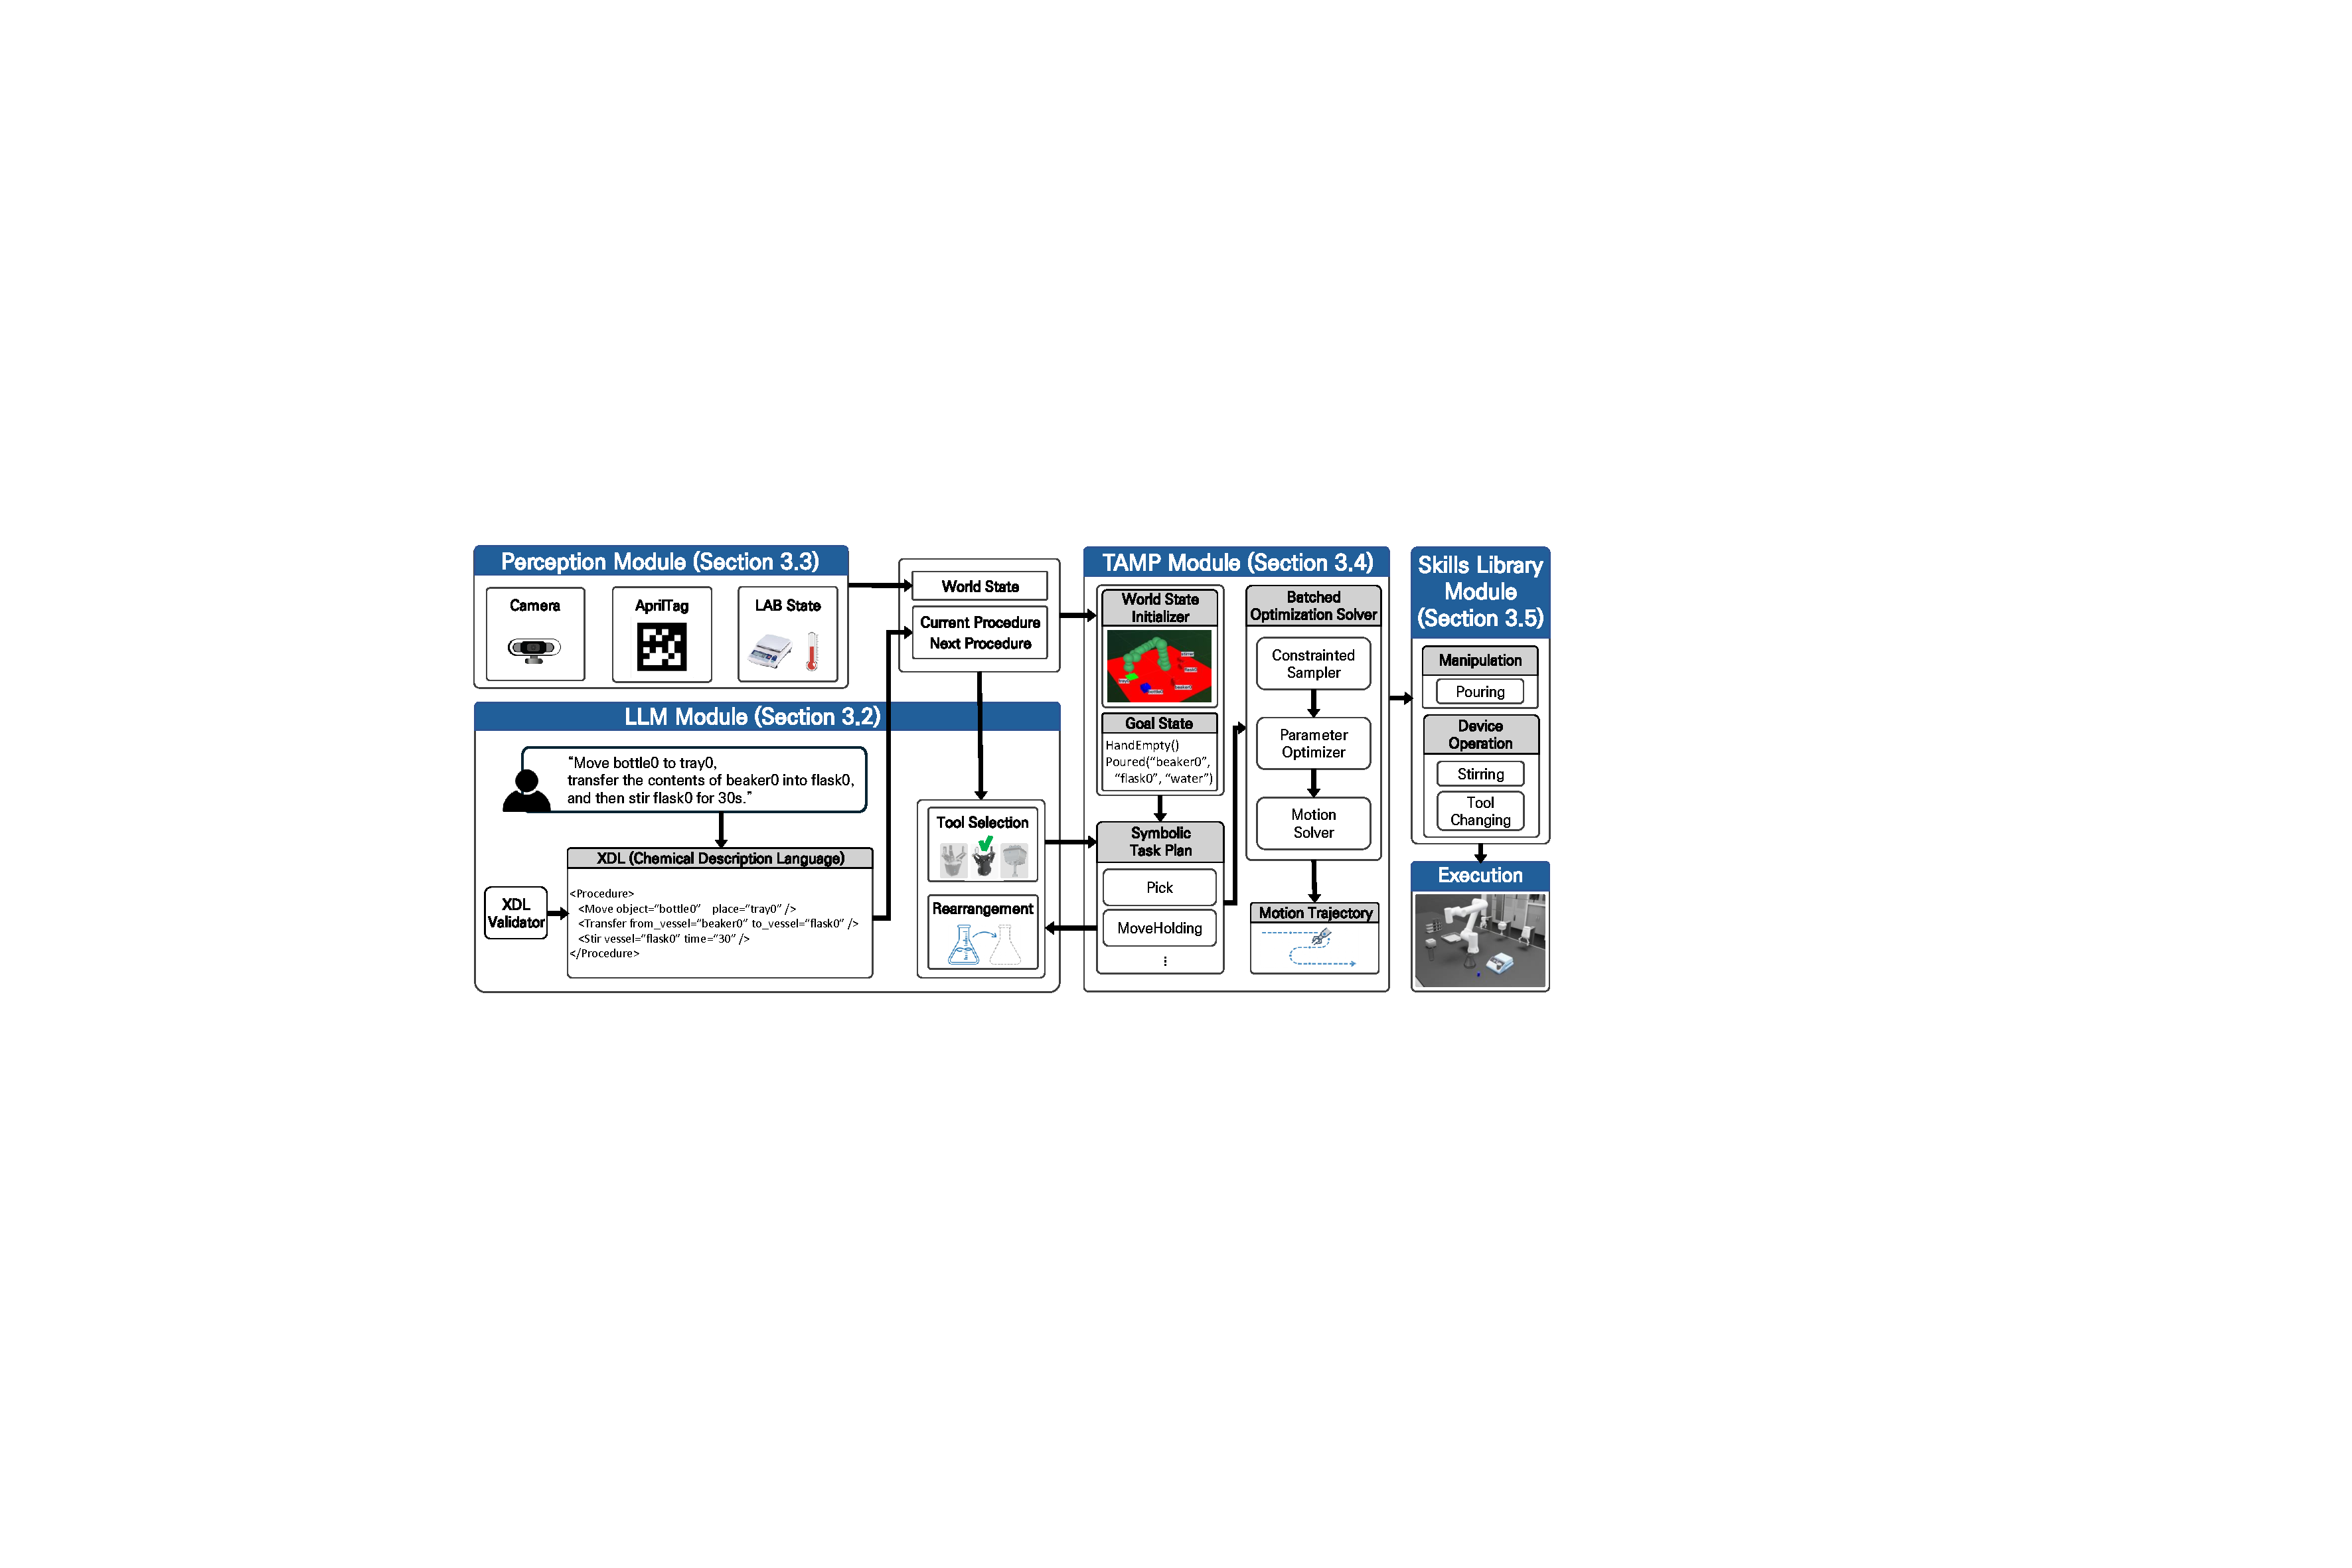
\includegraphics[width=\textwidth]{figures/figure1.pdf}
\caption{Architectural overview of the LLM-Guided Tool-Aware TAMP framework. The hierarchy illustrates the integration of symbolic reasoning (LLM Module) with physical execution (TAMP Module) supported by a multi-modal perception interface (Perception Module) and a robotic skill library (Skill Library Module).}\label{fig:fig.1}
\end{figure*}

\subsection{Large Language Models for Robot Planning and Embodied Decision-Making}\label{sec:2.3}
The advent of Large Language Models (LLMs) has opened new possibilities for translating abstract natural language commands into robot-executable instructions. Mehr et al. \cite{ref18} proposed the Chemical Description Language (XDL) standard for the digitization of chemical literature, and Yoshikawa et al. \cite{ref17} built the CLAIRify system, which uses LLMs to convert chemical texts into robot commands. Darvish et al. (ORGANA) \cite{darvish2025organa} presented an interactive robotic assistant that utilizes an LLM-based planner to converse with scientists and assist with experiments, and ChemCrow \cite{ref19} and Coscientist \cite{ref20} demonstrated that LLMs can autonomously search for chemical tools and design experimental procedures.

While these systems demonstrate strong capabilities in semantic decomposition and high-level task sequencing, their use of LLMs generally remains confined to text-based procedure generation or human decision-making assistance. The generated plans are typically handed off to a separate, manually configured execution pipeline, and the LLM itself is not required to reason about the physical execution environment, such as which end-effector is geometrically appropriate for a given vessel, or whether workspace obstacles must be rearranged before a procedure can proceed. As a consequence, geometric validity, collision avoidance, and orientation feasibility must be delegated entirely to downstream planning modules. This pattern is exemplified by general-purpose LLM-robotics interfaces such as that of Vemprala et al. \cite{vemprala2024chatgpt}, in which an LLM composes robot behaviors across manipulation and navigation tasks by invoking a predefined high-level function library, so that geometric feasibility and physical execution are resolved by that manually designed layer rather than reasoned about by the language model itself. Recent work has sought to close this gap through simulation-based feasibility verification. Qu et al. \cite{qu2026trtp} proposed TRTP, a three-stage framework that couples vision-language models with digital twin simulation to evaluate spatial reachability and physical feasibility of LLM-generated action sequences before execution. While this closed-loop architecture improves plan reliability, the feasibility check is performed in a separate simulation module rather than being resolved at the symbolic reasoning stage; end-effector selection and context-dependent obstacle rearrangement remain outside the scope of the language model's decision-making. This separation means that existing LLM-based robot planning systems can formulate what to do, but lack the ability to determine the execution context required to carry it out, namely which tool is appropriate for the current task and whether the workspace must be reconfigured before execution proceeds.


\subsection{Position of This Work}\label{sec:2.4}
Existing work has addressed individual aspects of autonomous chemistry from complementary directions. SDL and chemistry automation systems have demonstrated automated experimental execution, but remain largely protocol-specific and assume fixed tool configurations that require manual redesign for new procedures. Constrained TAMP approaches have tackled motion planning under geometric constraints, but exhibit reliability degradation on low-redundancy manipulators and do not guarantee bounded and predictable planning latency for time-sensitive chemical workflows. LLM-based robot planning systems have enabled high-level semantic reasoning for chemical procedures, but remain confined to protocol generation without determining the execution context required to carry out each procedure.

Limited attention has been paid to jointly addressing context-aware symbolic reasoning for end-effector selection, obstacle rearrangement, and procedural sequencing together with reliable, bounded-time constrained execution on general-purpose laboratory manipulators. The proposed framework is positioned at the intersection of these three directions, where it unifies LLM-based context-aware decision-making with batched joint differentiable optimization-based constrained planning within a single end-to-end system for flexible and reliable chemistry laboratory automation.



\section{Methods}\label{sec:3}
Section \ref{sec:2} identified three coupled limitations that prevent existing approaches from achieving flexible and reliable chemistry laboratory automation: existing automation pipelines require manual redesign whenever new apparatus or procedures are introduced; constrained motion planning on low-redundancy manipulators suffers from degraded reliability and unpredictable termination time under orientation constraints; and LLM-based robot planning systems remain confined to protocol generation without determining the execution context required to carry out each procedure, namely tool selection and obstacle rearrangement decisions.
To address these limitations, the proposed framework comprises four mutually necessary modules: the LLM Module, TAMP Module, Skill Library Module, and Perception Module. The LLM Module jointly addresses the first and third limitations by converting natural-language instructions into validated XDL protocols and determining the execution context required at each procedural stage, including end-effector selection and obstacle rearrangement, without requiring manual domain redefinition. The TAMP Module addresses the second by adopting cuTAMP \cite{shen2025differentiable} as its planning backbone, jointly optimizing batched candidate solutions through differentiable gradient descent to produce constraint-satisfying trajectories within a structurally bounded time budget. The Skill Library Module complements the TAMP Module by handling execution-level actions that are not amenable to geometric planning alone, such as adaptive pouring and temperature regulation, ensuring robust physical execution under real-world uncertainty. The Perception Module underpins all three by continuously sensing the laboratory environment and constructing a World State, a structured representation of object poses, environment geometry, and apparatus configurations that conforms to the symbolic and geometric world definition required by the TAMP Module. This representation is supplied to each module as required.

\subsection{Framework Overview}\label{sec:3.1}



Fig.~\ref{fig:fig.1} illustrates the overall architecture and inter-module data flow of the proposed framework, in which the LLM Module, TAMP Module, and Skill Library Module operate sequentially on the basis of a shared World State continuously maintained by the Perception Module, which senses object poses and sensor data throughout the laboratory environment.

The pipeline begins with the LLM Module converting the natural-language command into an XDL protocol. Since a linguistically valid protocol may still be physically infeasible in the current workspace, the protocol is cross-checked against the current World State before being passed to the execution stage. Prior to each XDL procedure, the LLM Module infers the required end-effector, whether obstacle rearrangement is necessary, the auxiliary end-effector for rearrangement, and the target location for the relocated object by referencing the latest World State. At this stage, the LLM specifies only the target workspace grid for rearrangement, while precise geometric computation is delegated to the TAMP Module.

The TAMP Module receives these symbolic decisions, constructs a task plan, and computes a collision-free, constraint-satisfying nominal trajectory for each operator by searching for a plan skeleton and using the latest World State. However, since geometric planning alone cannot account for physical uncertainties that arise during execution, such as liquid flow and contact dynamics, the nominal trajectories are passed to the Skill Library Module. The Skill Library Module translates the nominal trajectories into physical execution through sensor-feedback-based motion primitives, correcting for uncertainties not modeled at the planning stage in real time.

Each module completes its responsibilities within a well-defined scope before passing control to the next, thereby preventing failures at one level from propagating to subsequent stages. Sections \ref{sec:3.2} through \ref{sec:3.5} describe the internal structure and design principles of each module in detail.

\subsection{LLM Module}\label{sec:3.2}
The LLM Module constitutes the symbolic reasoning layer of the proposed framework, serving as the interface through which natural-language instructions are systematically translated into executable protocols and context-dependent execution decisions are resolved prior to physical planning. Central to its design is the deliberate confinement of the LLM to discrete symbolic outputs, a constraint motivated by a fundamental limitation of current language models: continuous 3D spatial reasoning, such as deriving exact placement coordinates or collision-free waypoints, lies outside their reliable operating regime and introduces the risk of geometrically infeasible outputs propagating into downstream execution. Rather than exposing the model to such reasoning demands, the module restricts its scope to decisions that are inherently symbolic in nature, whose outputs belong to a finite, discrete set and require no continuous spatial computation: selecting an end-effector from a predefined inventory, determining whether obstacle rearrangement is necessary, and specifying a target workspace grid rather than a precise Cartesian location. The geometric realization of these abstract decisions, most notably exact placement within the designated workspace grid, is delegated to the TAMP Module, which operates at the continuous spatial level; this division of labor positions the LLM at an abstraction level commensurate with its pattern-matching capabilities, while systematically preventing hallucinated spatial quantities from entering the planning pipeline.

Organized around this design principle, the module proceeds through three sequential stages. The XDL Generator synthesizes a global experimental protocol from the input natural-language command, producing a structured symbolic representation of the intended procedure. The XDL Validator then performs three progressively stricter checks: syntactic validation, object-existence verification, and physical-feasibility assessment. By intercepting language-level inconsistencies at this stage, the validator ensures that only coherent and physically grounded protocols advance to execution. Finally, the Action Reasoner analyzes the current World State in conjunction with procedural context to infer tool selection and obstacle rearrangement decisions at each procedural step. The following subsections describe each of these stages in detail.

\subsubsection{Global Experimental Protocol Synthesis}\label{sec:3.2.1}
The XDL Generator functions as a schema-constrained protocol generation module that maps natural-language commands into complete, end-to-end structured XDL programs encoding the full experimental procedure in a single pass. This global synthesis approach is a direct instantiation of the discrete-output design principle: by confining the output space to a fixed XDL schema with a finite set of operators and parameter types, the generator is discouraged from producing continuous spatial quantities, substantially reducing the risk of geometrically infeasible outputs propagating into downstream execution. The discreteness of the schema also means that a lightweight \textit{Llama 3.2 1B} model fine-tuned via Low-Rank Adaptation (LoRA)-based supervised fine-tuning (SFT) is sufficient to achieve reliable conversion without the overhead and latency of general-purpose large models. The training dataset consists of 5,000 manually constructed samples covering synonym variations for six core XDL operators, continuous numerical parameter ranges, and diverse object instances. Additional details on dataset construction and training are provided in Section \ref{sec:4.1.3}.

\begin{figure*}[!t]
\centering
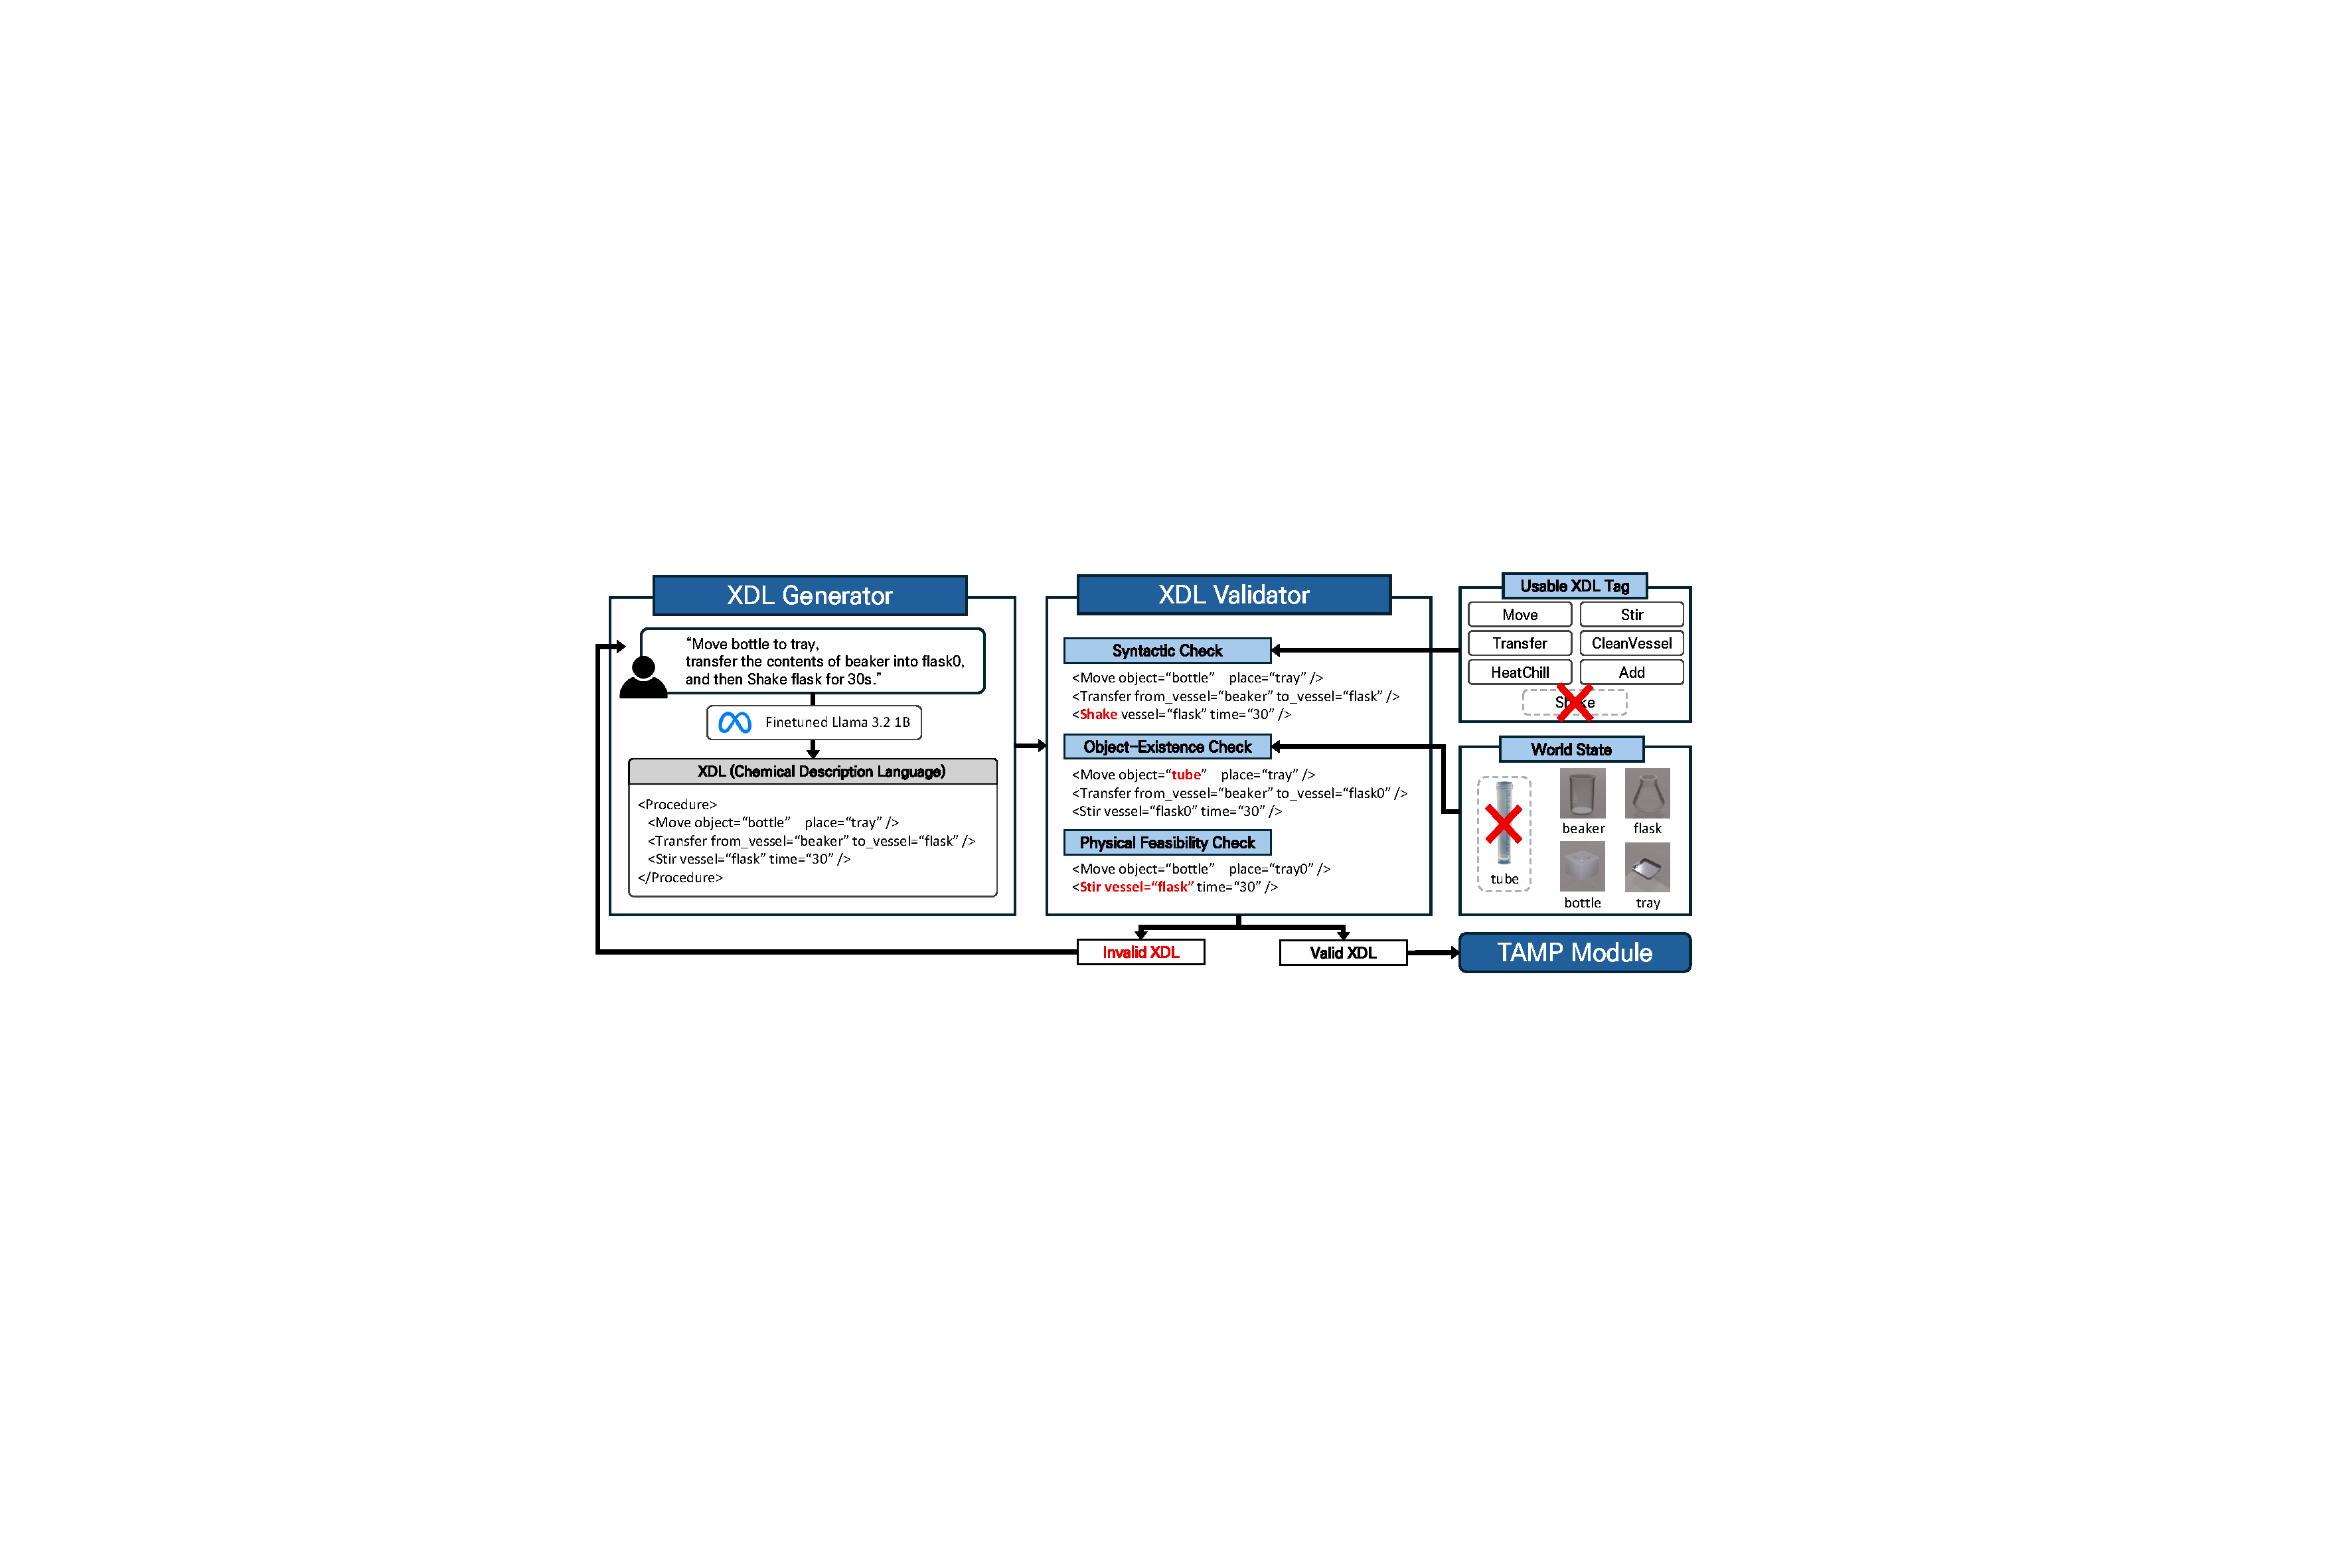
\includegraphics[width=0.95\textwidth]{figures/figure2.pdf}
\caption{The XDL Generator and Validator pipeline within the LLM Module. A fine-tuned \textit{Llama~3.2~1B} model converts a natural language command into a structured XDL protocol, which is then subjected to three progressively stricter checks (syntactic, object-existence, and physical-feasibility) before a valid protocol is forwarded to the TAMP Module.}\label{fig:fig.2}
\end{figure*}

\begin{figure*}[!t]
\centering
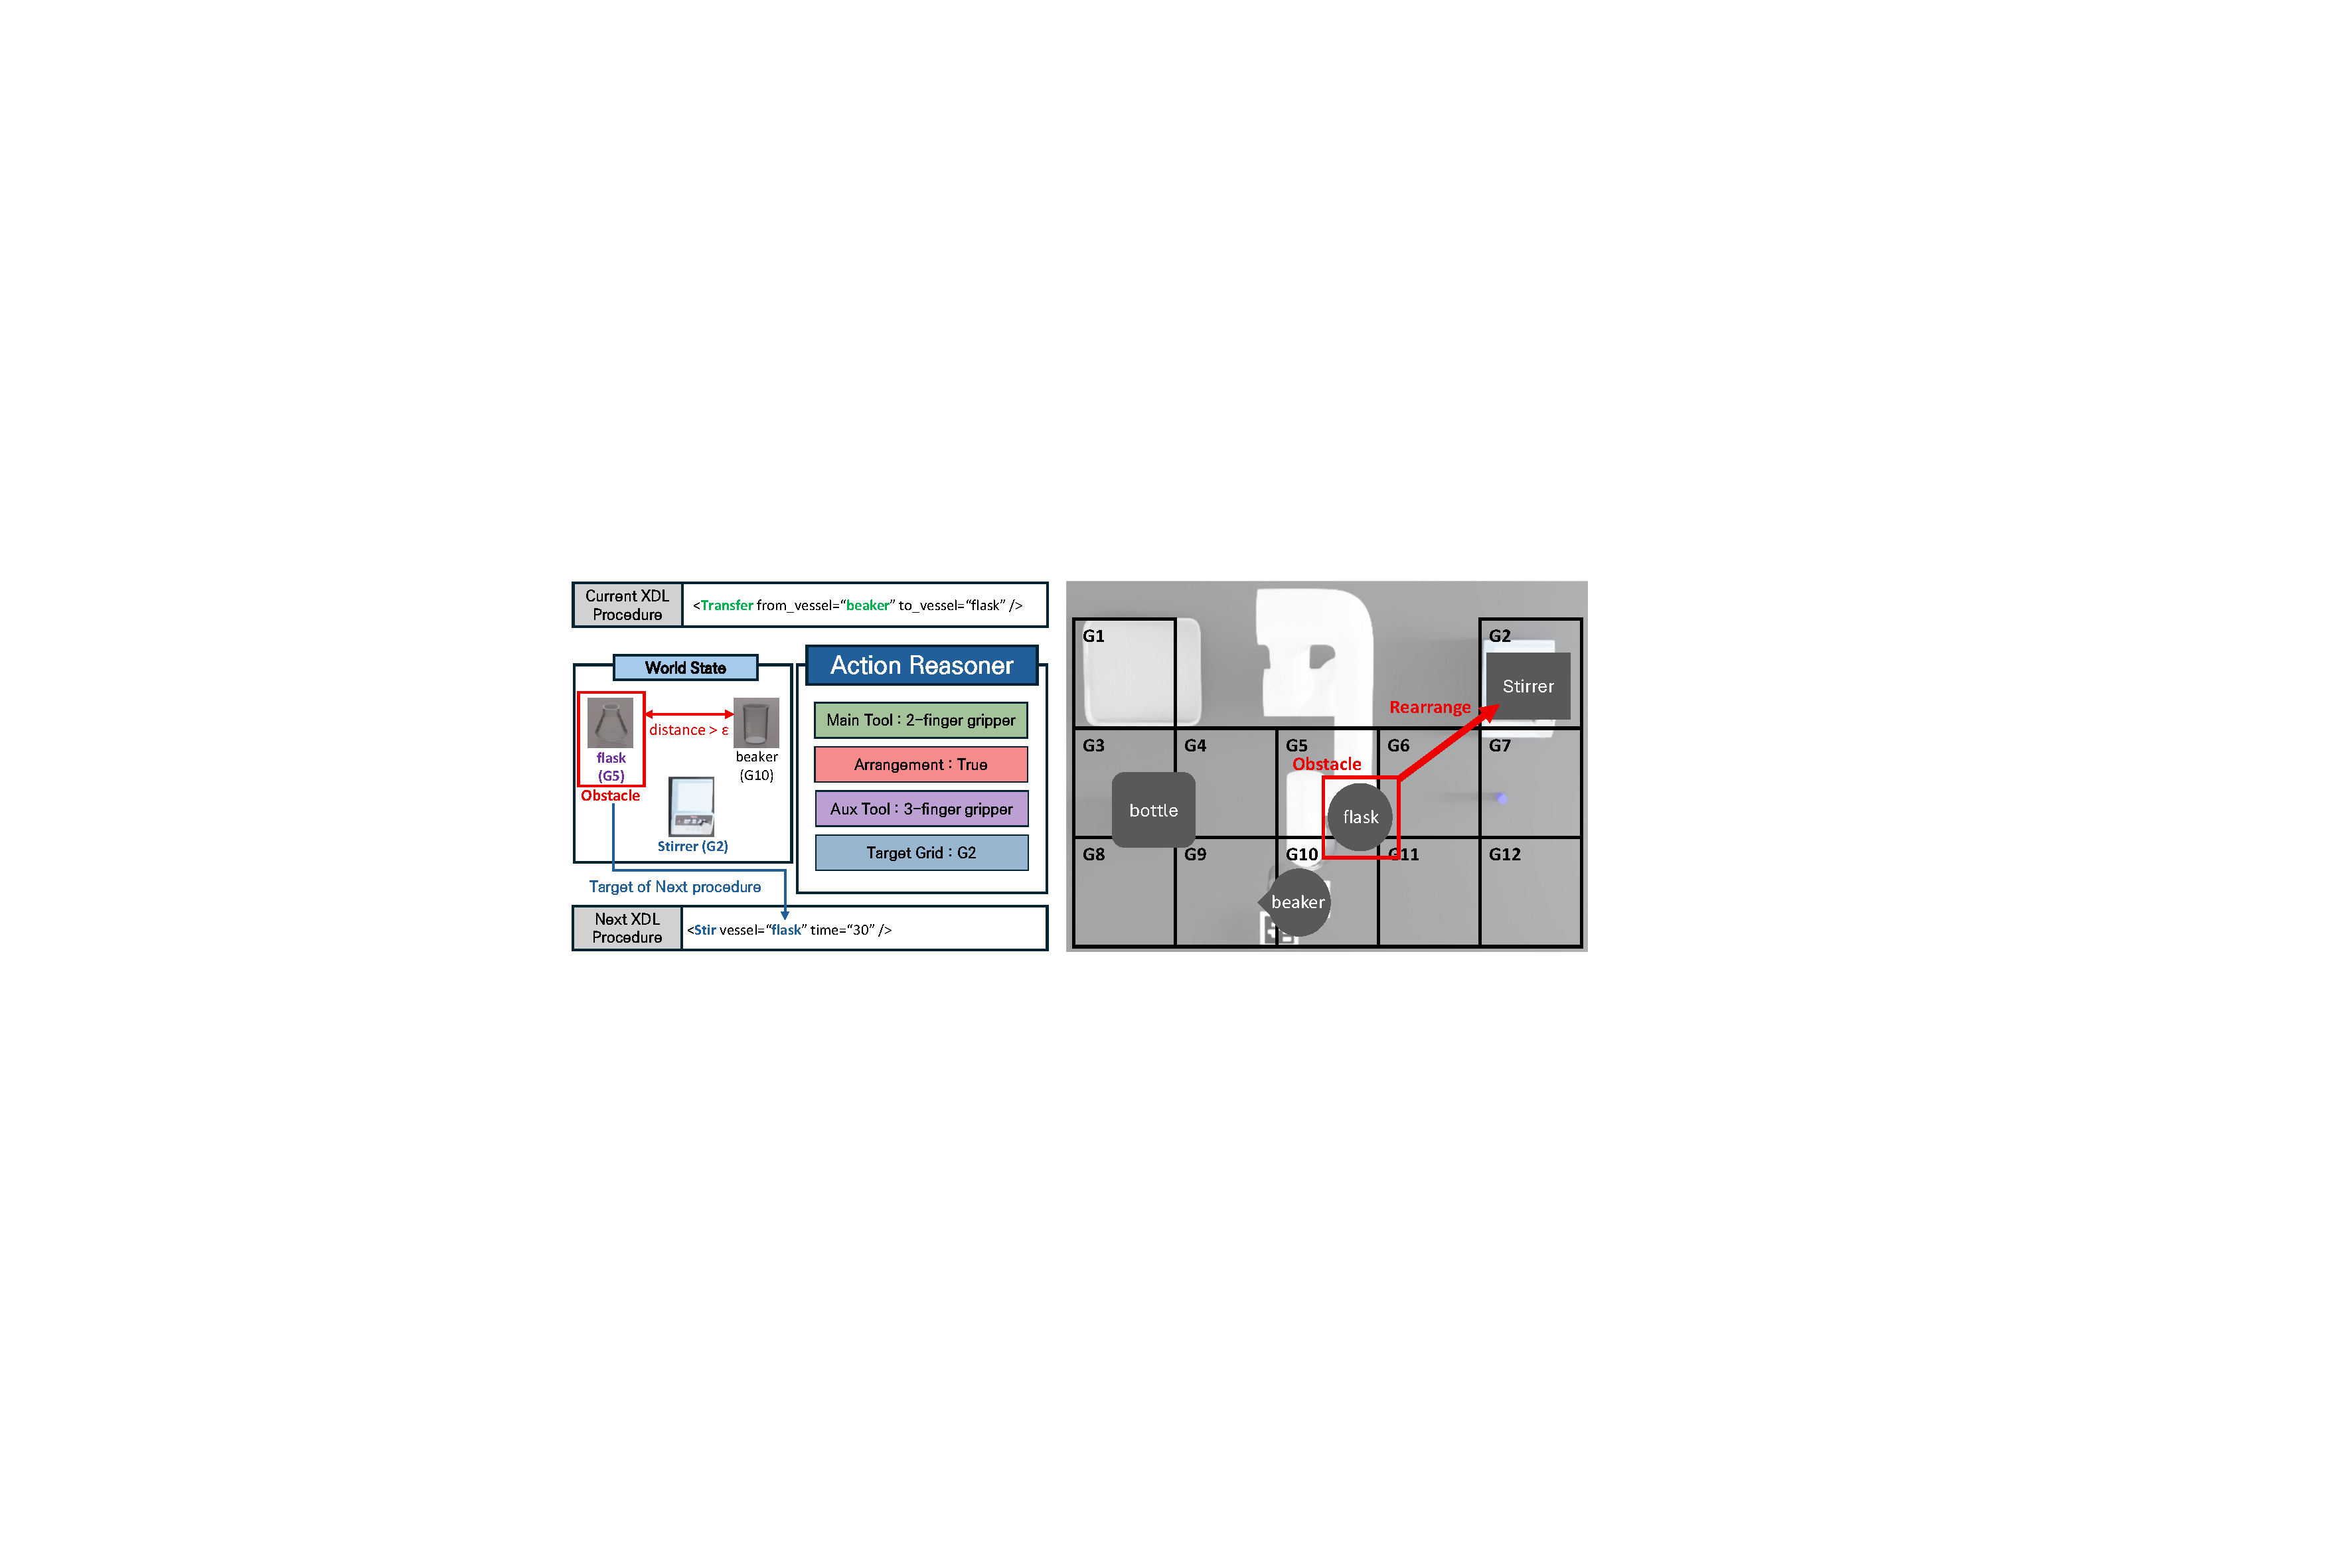
\includegraphics[width=0.9\textwidth]{figures/figure3.pdf}
\caption{Illustration of the Action Reasoner pipeline. Given the current and next XDL procedures alongside the World State, a fine-tuned \textit{Llama~3.2~1B} model infers four discrete outputs: the main end-effector, whether obstacle rearrangement is necessary, the auxiliary tool for rearrangement, and the target workspace grid within the discretized workspace (G1--G12).}
\label{fig:fig.3}
\end{figure*}

\subsubsection{Protocol Validation}\label{sec:3.2.2}
The XDL Validator serves as the safety interface between the language layer and the physical execution pipeline. While the XDL Generator produces structured protocols, a protocol that is syntactically valid may still be physically infeasible. The Validator therefore enforces three progressively stricter checks before any robot motion is executed. Syntactic validation verifies well-formed XML structure and permitted operator tags, blocking case-sensitivity mismatches and undefined elements. Object-existence validation cross-references all referenced objects against the workspace inventory provided by the Perception Module, intercepting commands that refer to objects absent from the current environment. Physical-feasibility validation simulates the content state of each vessel across the procedure and rejects sequences that violate procedural preconditions, such as stirring an empty vessel or transferring from an empty source. If a conflict is detected at any stage, execution is halted and the offending step and error type are reported to the user, enabling targeted protocol-level revision before physical failure can occur. Fig.~\ref{fig:fig.2} illustrates representative examples: syntactic validation rejects undefined operator tags such as Shake, object-existence validation intercepts references to absent objects such as tube, and physical-feasibility validation rejects operations such as stirring an empty vessel.

\begin{figure*}[!t]
\centering
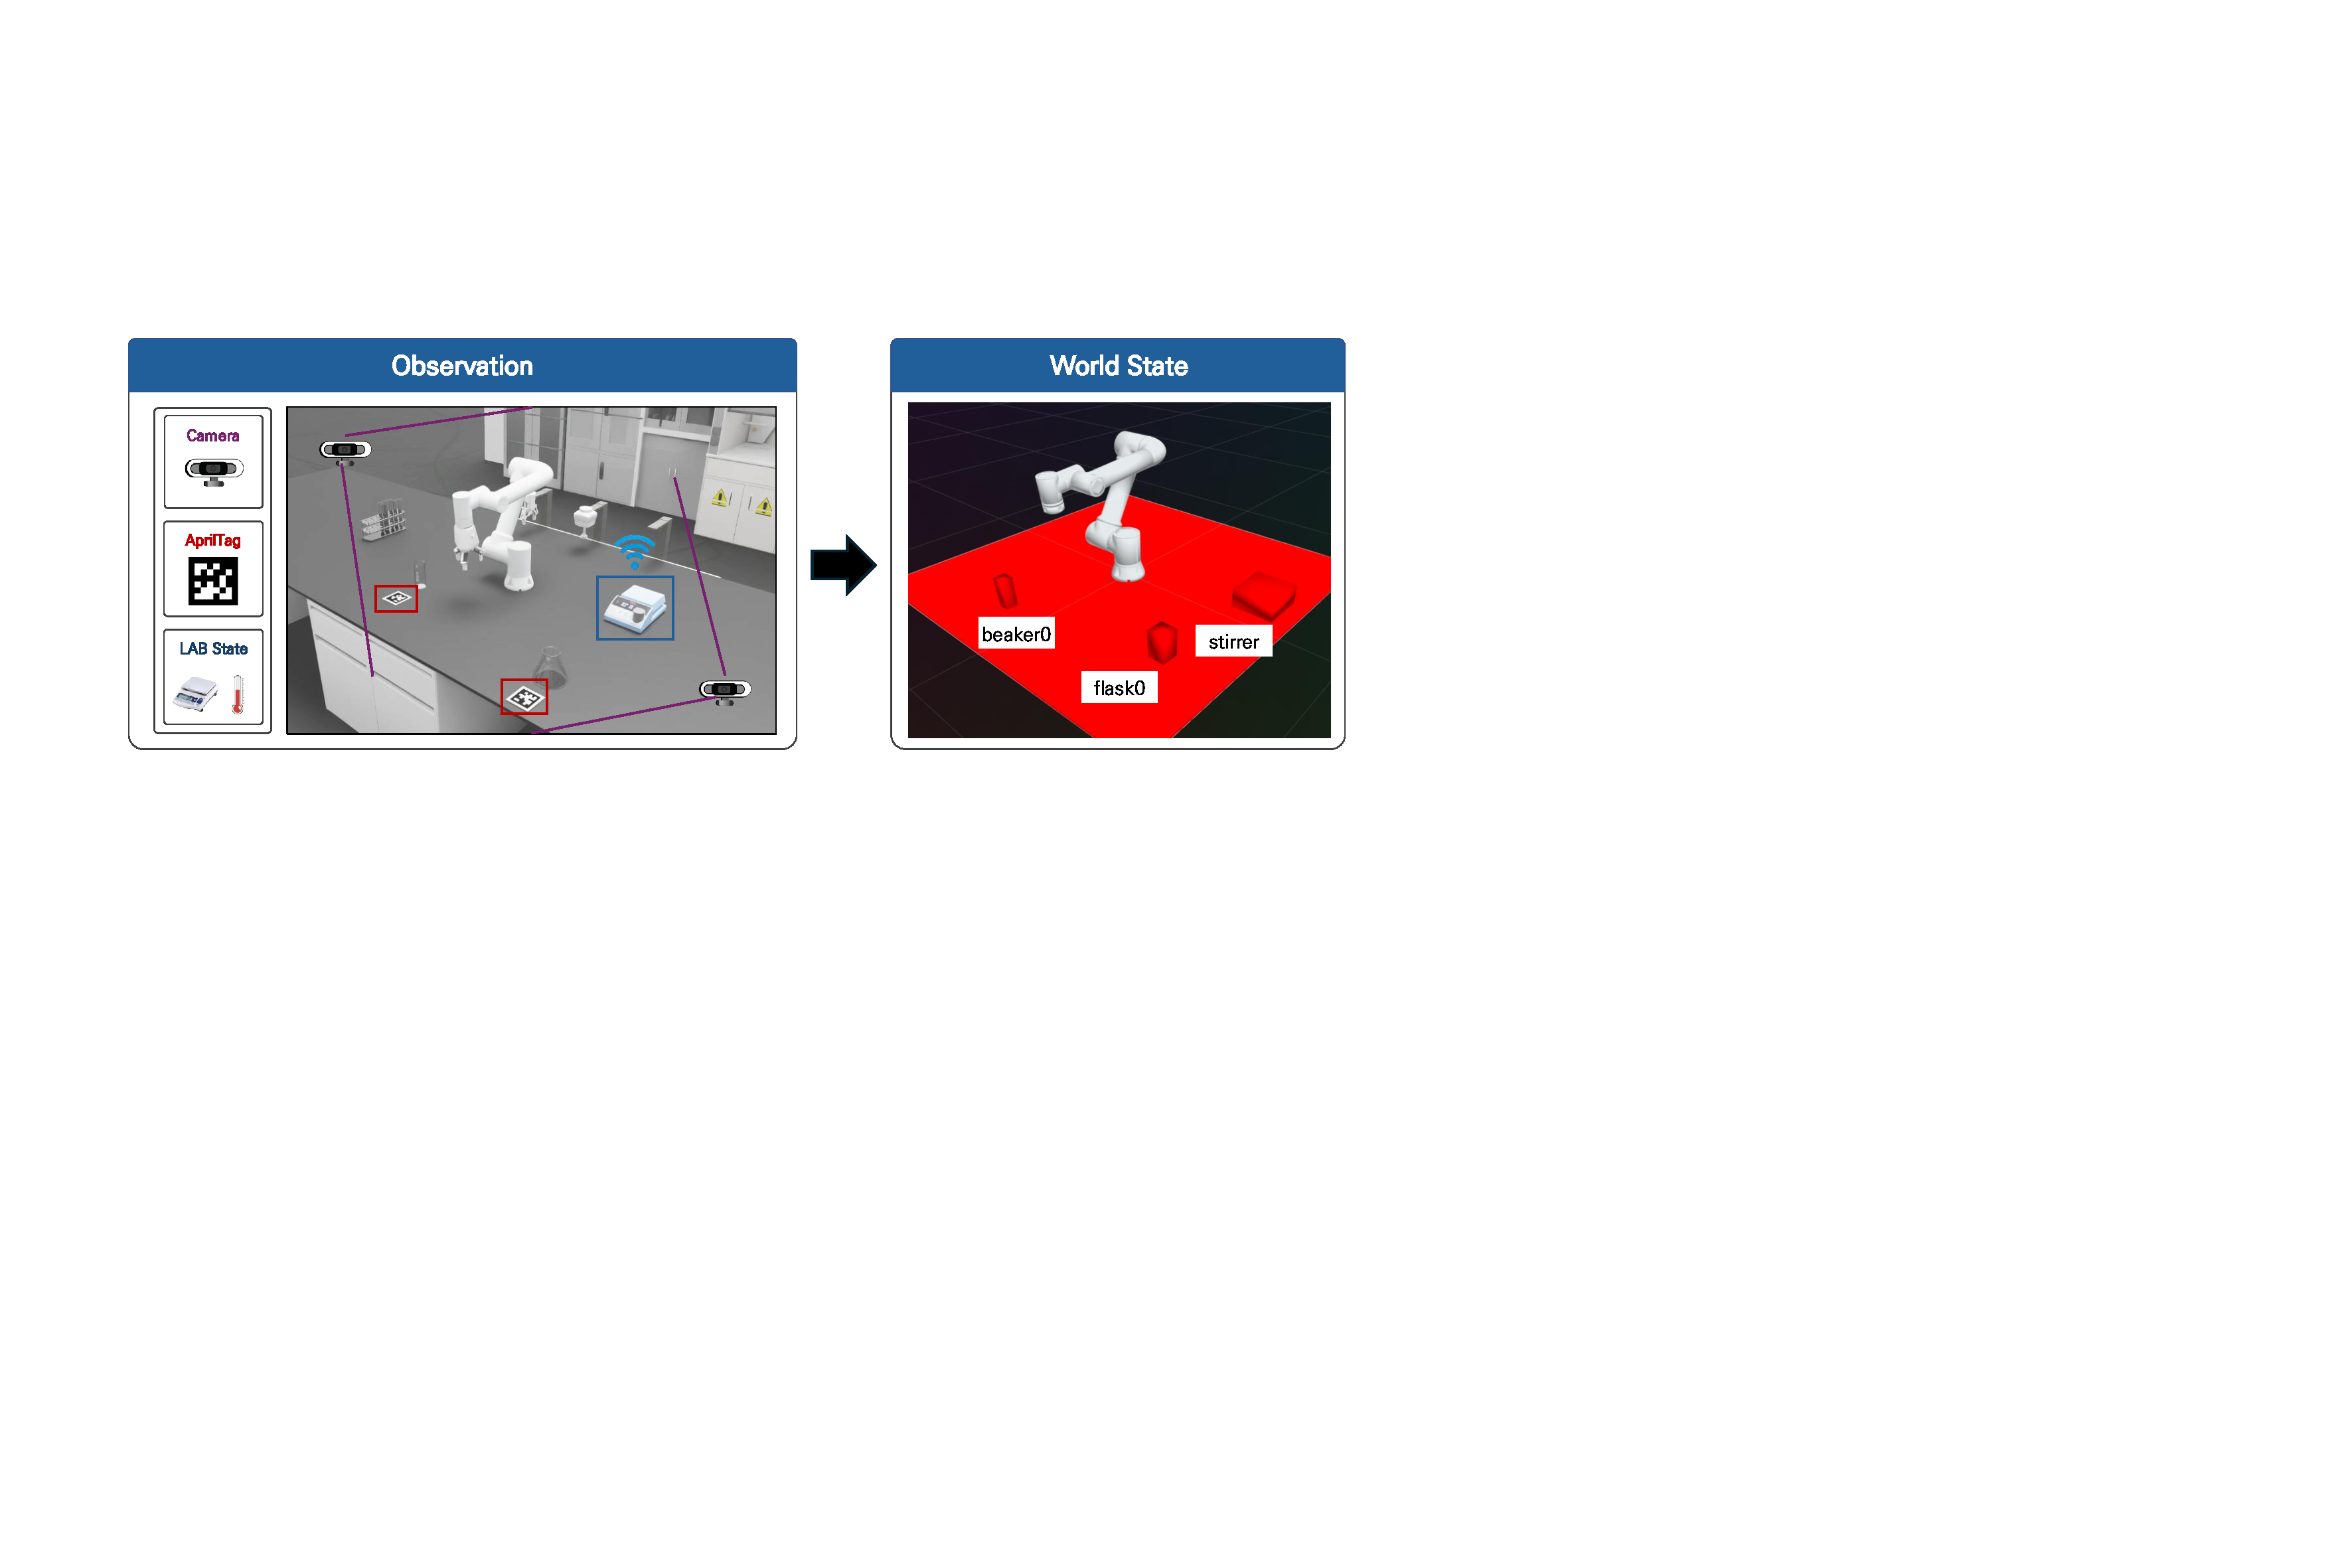
\includegraphics[width=\textwidth]{figures/figure4.pdf}
\caption{Overview of the Perception Module pipeline. Multi-view observations of the laboratory environment are fused and transformed into a World State, providing downstream modules with consistent 6-DoF pose estimates of laboratory assets.}
\label{fig:fig.4}
\end{figure*}

\subsubsection{Context-Aware Tool and Action Reasoning}\label{sec:3.2.3}

The Action Reasoner determines the end-effector and obstacle rearrangement strategy for each procedure before the TAMP Module begins planning. This stage is critical for reducing planning failures caused by tool mismatches or obstructed workspaces. Following the symbolic-level design principle established in Section \ref{sec:3.2}, the module operates on the discretized workspace representation illustrated in Fig.~\ref{fig:fig.3}, where the environment is partitioned into 12 workspace grids (G1--G12) based on the spatial state provided by the Perception Module. A fine-tuned \textit{Llama 3.2 1B} model receives four inputs: the current XDL procedure, the subsequent procedure, the current obstacle layout, and the workspace grid state. From these, it infers four discrete decision variables: the required end-effector for the current operation, whether preliminary object rearrangement is necessary, the auxiliary tool for rearrangement, and the target workspace grid for the relocated object.

This design provides two main advantages. First, it enables semantic tool assignment by grounding the model's knowledge of object affordances in the physical constraints of the available end-effectors. Consequently, appropriate grippers can be assigned even for vessel types unseen during training, minimizing the need for manual domain redefinition. Second, it enables context-aware rearrangement by jointly considering the current and subsequent procedures, allowing obstacles to be moved proactively toward regions required for future steps and thereby reducing redundant rearrangements. Because auxiliary rearrangement does not demand high positional precision, the Action Reasoner predicts only the target workspace grid, while exact placement within that region is delegated to the TAMP Module. This clear division of labor ensures that the LLM handles high-level strategy while the TAMP Module ensures geometric and kinematic feasibility. For example, as illustrated in Fig.~\ref{fig:fig.3}, when the flask obstructs access to the beaker in the current procedure, and the next procedure is a Stir operation targeting the flask, the Action Reasoner identifies the flask as an obstacle requiring rearrangement and infers G2 as the target grid, since the stirrer is located there.

\subsubsection{Containment of Language-Model Errors}\label{sec:3.2.4}
\rev{Language models can produce outputs that are fluent but wrong, and the LLM Module is designed so that such an output cannot reach the robot.
Five mechanisms act in layers, each exercised by an experiment in Section~\ref{sec:4}; Table~\ref{tab:containment} summarizes the correspondence.}

\rev{First, both LLM components are trained to emit only elements of finite sets: the XDL Generator six operators with typed attributes, and the Action Reasoner a tool inventory, a boolean, and a grid index.
Decoding is not grammar-constrained, so a malformed or out-of-schema output can in principle occur; what the design guarantees is that such an output cannot reach the planner, because every output is parsed against the schema by a deterministic checker before use, and no language model ever produces a continuous spatial quantity.
Second, the three-layer XDL Validator (Section~\ref{sec:3.2.2}) rejects any protocol that references an object absent from the perception inventory or requires an impossible vessel state before planning begins; object existence is checked against the observed World State, not against the model's own belief.
Third, the geometric realization of every symbolic decision is performed by cuTAMP through collision-checked optimization, which reports infeasibility rather than executing an invalid placement.
Fourth, the World State is refreshed from perception before every procedure (Algorithm~\ref{algo:tamp}), so a wrong assumption at one stage cannot persist silently into the next.
Fifth, every rejection halts the workflow with a diagnostic naming the offending step; the system never proceeds on an unverified plan.
The residual exposure is the class of instructions that are ambiguous yet schema-valid and precondition-consistent, which is characterized in Section~\ref{sec:5.3}.}

\begin{table}[t]
\revbox{%
\centering
\caption{Containment of language-model errors: each mechanism and the experiment that exercises it.}\label{tab:containment}
\begin{tabular*}{\linewidth}{@{\extracolsep{\fill}}p{0.47\linewidth}p{0.45\linewidth}@{}}
\toprule
Mechanism & Evidence \\
\midrule
Discrete, schema-bounded outputs & Zero out-of-schema outputs in 100 protocols (Sec.~\ref{sec:4.2.1}) \\
Three-layer validation against the World State & Zero false negatives on injected errors (Sec.~\ref{sec:4.2.2}) \\
Geometric realization by optimization & 100\% category-level grid accuracy (Sec.~\ref{sec:4.4.1}) \\
Stage-wise re-grounding & Planning and execution rates coincide (Sec.~\ref{sec:4.5}) \\
Fail-closed halting & Diagnostic returned for every rejection (Sec.~\ref{sec:4.2.2}) \\
\bottomrule
\end{tabular*}}
\end{table}



\subsection{Perception Module}\label{sec:3.3}

The Perception Module serves as the primary interface for world-state grounding, supplying all downstream modules with a consistent and up-to-date representation of the laboratory environment. Its primary role is to provide the TAMP Module with real-time 6-DoF pose information of laboratory assets for collision-free motion planning, but its outputs are consumed more broadly across the framework: the LLM Module's Action Reasoner relies on the workspace grid state for context-aware tool and rearrangement decisions, and the Skill Library Module draws on continuous sensor streams for closed-loop execution of skills such as adaptive pouring and temperature regulation.

Precise and reliable localization of apparatus is critical for ensuring safe and collision-free manipulation in an autonomous chemistry environment. The module adopts an \textit{AprilTag}-based strategy \cite{wang2016apriltag} to achieve robust pose estimation at low computational latency, as illustrated in Fig.~\ref{fig:fig.4}. Markers are rigidly affixed to each vessel, and their poses are continuously estimated from two spatially diverse, calibrated RGB cameras mounted around the workspace; fusing observations from multiple viewpoints in this manner follows established multi-view planar-marker tracking approaches \cite{sarmadi2019simultaneous} that improve pose consistency and robustness to occlusion relative to single-camera estimation. The following subsections detail the localization pipeline, world-state construction, and sensor stream processing that together constitute the module's output.


\subsubsection{Lab Object Localization}\label{sec:3.3.1}
Each lab object is assigned a unique identifier, and its localization proceeds through a three-stage pipeline: individual pose computation in the robot base frame, dual-camera fusion for robustness against occlusions, and tag-to-vessel coordinate transformation.

\textbf{Single-Camera Pose Computation}: For each camera $c \in \{1, 2\}$, the pose of object $i$ in the robot base frame is obtained by chaining the fixed extrinsic calibration ${}^{\text{b}}T_{c}$ with the detected marker pose ${}^{c}T_{\text{t}}^{(i)}$. To assess observation reliability, the Euclidean distance $d_c^{(i)}$ from the camera optical center to the marker is recorded as a weight metric:
\begin{equation}
    {}^{\text{b}}T_{\text{t},c}^{(i)} = {}^{\text{b}}T_{c} \cdot {}^{c}T_{\text{t}}^{(i)}, \quad
    d_c^{(i)} = \bigl\|\mathbf{t}\bigl({}^{c}T_{\text{t}}^{(i)}\bigr)\bigr\|_2.
\end{equation}

\textbf{Inverse-Distance Weighted Fusion}: When both cameras yield valid observations, the estimates are fused by assigning higher confidence to the camera closer to the marker, thereby minimizing distance-dependent projection errors. Given a regularization constant $\varepsilon = 10^{-6}$ to prevent division by zero, the normalized weights $W_c$ and the resulting fused translation $\tilde{\mathbf{t}}$ and orientation $\tilde{\mathbf{q}}$ via Spherical Linear Interpolation (\textit{SLERP}) \cite{lynch2017modern} are computed as follows:
\begin{equation}
\begin{aligned}
    W_c &= \frac{(d_c^{(i)})^{-2}}{\sum_{j=1}^{2} (d_j^{(i)})^{-2} + \varepsilon}, \\
    \tilde{\mathbf{t}} &= W_1\mathbf{t}_1 + W_2\mathbf{t}_2, \quad
    \tilde{\mathbf{q}} = \mathrm{\textit{SLERP}}(\mathbf{q}_1, \mathbf{q}_2, W_2).
\end{aligned}
\end{equation}
If occlusion occurs and only one camera provides a valid observation, its estimate is used directly without fusion to maintain continuity of pose tracking.

\textbf{Tag-to-Object Offset Transform}: Since markers are affixed to the side surfaces of vessels rather than their geometric centers, a fixed rigid offset ${}^{\text{t}}T_{\text{o}}$ is applied to recover the true physical center of the object:
\begin{equation}
    {}^{\text{b}}T_{\text{o}}^{(i)} = {}^{\text{b}}\tilde{T}_{\text{t}}^{(i)} \cdot {}^{\text{t}}T_{\text{o}}.
\end{equation}
The resulting transform ${}^{\text{b}}T_{\text{o}}^{(i)}$ is broadcast over the ROS~2 TF tree at 30\,Hz. These localized poses form the raw spatial foundation from which the World State is assembled, as described in Section \ref{sec:3.3.2}.

\subsubsection{State Grounding and World Modeling}\label{sec:3.3.2}

The 6-DoF poses broadcast by the Perception Module are assembled into the World State, a unified environmental representation that the TAMP Module consumes for motion planning. The World State is initialized at the beginning of each XDL procedure and updated after every stage transition, ensuring that the planner always operates on the current laboratory configuration.
\rev{Each update requires a fresh detection of every object involved in the next procedure; if no valid detection is obtained in either view within \nd{5\,s}, the system halts and reports the affected object rather than planning on a stale pose, while a pose retained during motion is used for monitoring only.} To populate the World State, the module partitions all objects in the workspace into two categories: target objects designated for manipulation in the current stage, and non-target objects treated as obstacles. Static elements such as tables and laboratory equipment are maintained as fixed obstacles, while movable objects such as beakers, bottles, and flasks are dynamically refreshed from the latest Perception Module output at each update. To keep planning tractable as the number of laboratory objects grows, all object models are represented using simplified geometric primitives rather than full CAD geometries. Target objects are approximated as axis-aligned boxes or cylinders, while non-target obstacles are modeled as slightly enlarged primitives to provide a conservative collision margin. This abstraction reduces the computational burden of collision checking and path sampling while preserving execution feasibility, allowing the TAMP Module to scale to cluttered laboratory environments without a corresponding increase in planning overhead.


\subsubsection{Multi-Modal Sensor Stream Processing}\label{sec:3.3.3}

Beyond geometric world-state grounding, the Perception Module acts as a centralized telemetry hub that aggregates, filters, and distributes continuous data streams from various physical sensors. This real-time sensor processing is critical for closing the control loop in the Skill Library Module during physical execution, such as in adaptive pouring or temperature regulation. The module primarily processes two sensory modalities:

\textbf{Scale Data}: For precise quantitative liquid transfer, the module interfaces with an electronic precision scale. The raw weight measurements are acquired, synchronized with the system clock, and processed into a stable data stream. This filtered scale data is directly consumed by the Adaptive Pouring skill, serving as the primary feedback variable for the proportional-derivative (PD) controller to dynamically adjust the robot's wrist angle.

\textbf{Temperature Data}: To ensure strict adherence to chemical reaction conditions, the module also integrates temperature readings from external laboratory equipment, such as hotplate thermocouples. Raw temperature readings are monitored and smoothed to reject transient electrical noise. This provides a stable thermal state stream, which the device operation skills utilize to verify reaction temperatures and, if necessary, suspend task execution until the target thermal conditions are met.

By consolidating and filtering these heterogeneous data streams, the Perception Module shields the high-level planning and execution modules from hardware-specific noise, providing a clean and synchronized sensory interface for complex chemical manipulation.

\subsection{Task and Motion Planning Module}\label{sec:3.4}
The TAMP Module computes collision-free, constraint-satisfying trajectories for multi-step manipulation procedures in chemistry experiments while keeping planning latency structurally bounded and predictable, as required by time-sensitive chemical workflows. As reviewed in Section \ref{sec:2.2}, the PDDLStream-based approach \cite{bib5}, which attempts to bind each continuous parameter independently, is structurally ill-suited to these requirements. To address this limitation, the TAMP Module is designed as an integrated planning framework that combines cuTAMP \cite{shen2025differentiable} with chemistry-specific operators and an LLM-guided tool-switching mechanism.

\subsubsection{Chemistry-Specific TAMP}\label{sec:3.4.1}
The TAMP Module adopts cuTAMP as its planning solver, formulating the planning problem as a parallelized differentiable optimization process that simultaneously drives a large batch of candidate particles toward the constraint manifold via gradient-based optimization. Unlike approaches that attempt to bind each parameter independently, cuTAMP jointly optimizes all constraints across batched candidate solutions, enabling convergence toward the feasible region even under tight orientation constraints on low-redundancy manipulators. By executing a fixed number of optimization steps over a fixed batch of particles, the runtime remains structurally bounded and predictable, ensuring that planning delays do not disrupt time-sensitive reaction conditions such as temperature control and reagent timing.

\begin{figure*}[!t]
\centering
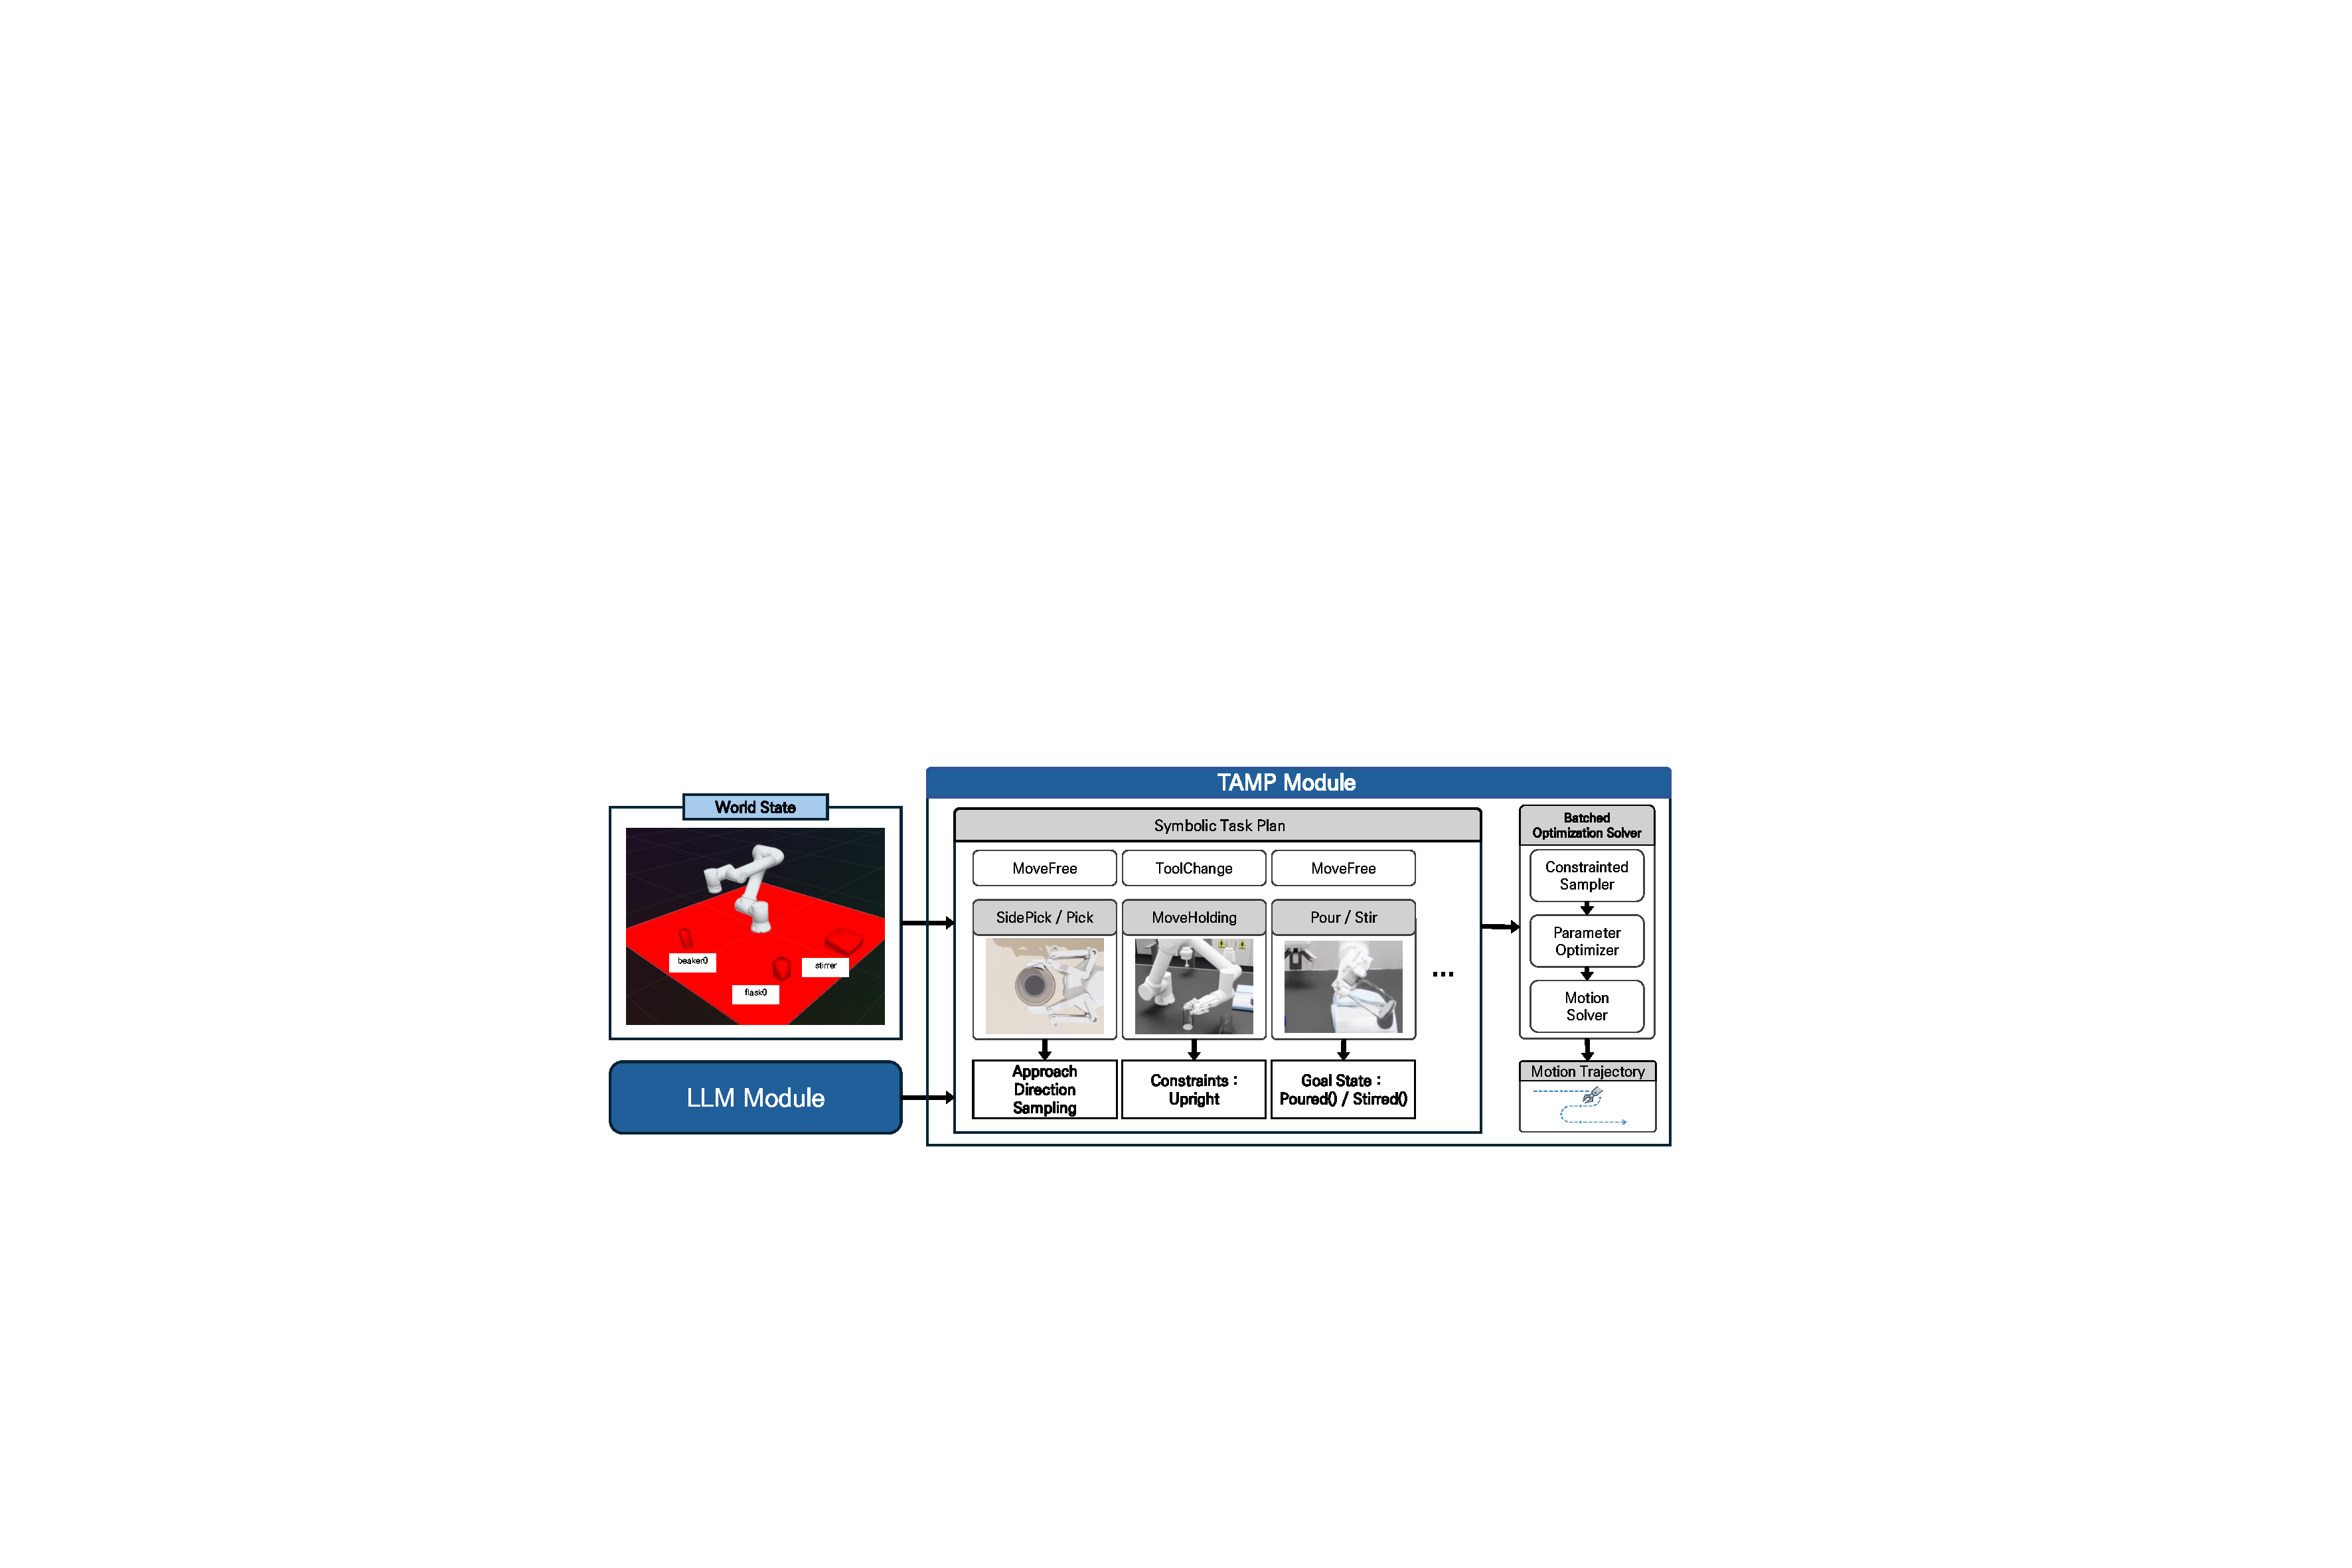
\includegraphics[width=0.95\textwidth]{figures/figure5.pdf}
\caption{Overview of the TAMP Module. The World State and the symbolic task plan, comprising chemistry-specific operators (SidePick, MoveHolding, Pour, Stir) alongside base operators (MoveFree, Pick), are passed to the Batched Optimization Solver, which sequentially executes a Constrained Sampler, Parameter Optimizer, and Motion Solver to produce the final motion trajectory.}
\label{fig:fig.5}
\end{figure*}

\begin{figure*}[!t]
\centering
\subfloat[\label{fig:fig.6a}]{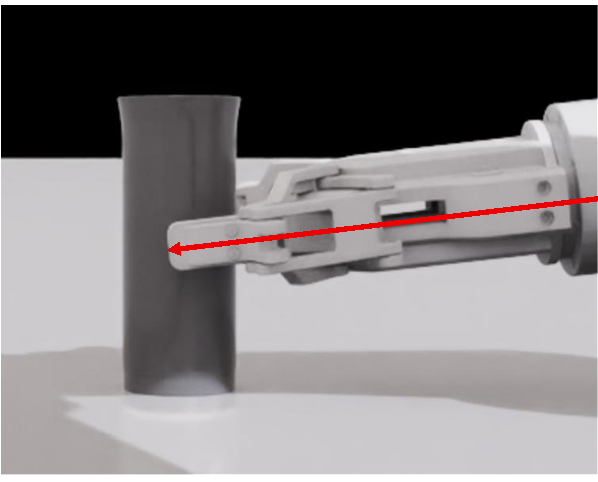
\includegraphics[width=0.31\textwidth]{figures/figure6a.pdf}}
\hfil
\subfloat[\label{fig:fig.6b}]{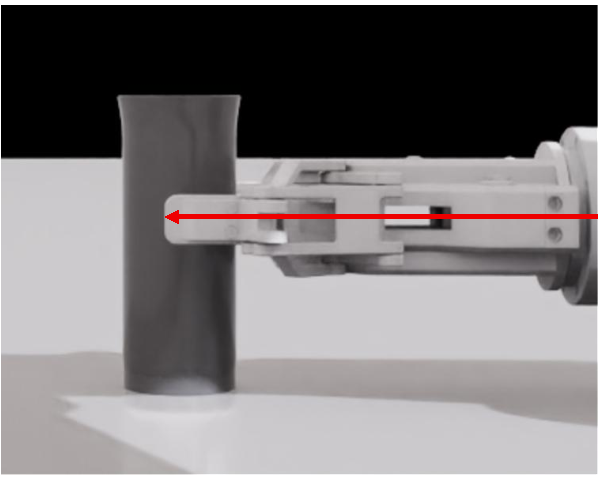
\includegraphics[width=0.31\textwidth]{figures/figure6b.pdf}}
\hfil
\subfloat[\label{fig:fig.6c}]{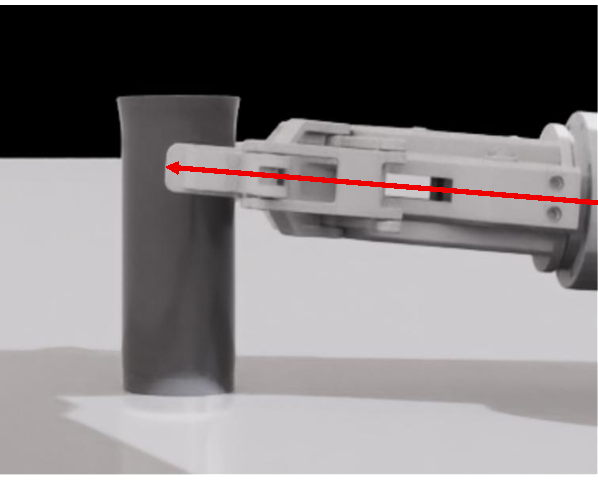
\includegraphics[width=0.31\textwidth]{figures/figure6c.pdf}}
\caption{Discrete yaw candidates for the SidePick operator, illustrating how gripper tilt varies across the sampled configurations. (a) $y = -\pi/2.5$, (b) $y = \pi/2$ (or $-\pi/2$), (c) $y = \pi/2.5$.}
\label{fig:fig.6}
\end{figure*}

Chemistry laboratory manipulation imposes requirements beyond those of general pick-and-place tasks. Cylindrical vessels must be grasped stably despite their geometry, liquids must be transported without spillage and transferred in precise quantities, and device-level operations such as stirring must be coordinated within the planning pipeline. To meet these requirements, we introduce four chemistry-specific operators in addition to the base TAMP operators: SidePick, for grasping the lateral surface of cylindrical vessels such as beakers and flasks; MoveHolding, for maintaining an upright orientation throughout the trajectory during liquid transport; Pour, for planning the tilting motion after the robot reaches the top of the target vessel; and Stir, a device-level operator for controlling the magnetic stirrer. Fig.~\ref{fig:fig.5} illustrates the overall structure of the TAMP Module, showing how chemistry-specific operators are composed into a symbolic task plan and resolved by the batched optimization pipeline.

The purpose of SidePick is to enable stable grasping of cylindrical vessels from any approach direction, where top-down grasping would otherwise be insufficient. In the object coordinate frame, where the z-axis is aligned with the vertical axis of the cylindrical vessel and the origin is located at the geometric center of the object, a grasp pose $\mathbf{g} = (\mathbf{t}, \mathbf{r})$ consists of translation $\mathbf{t} \in \mathbb{R}^3$ and orientation $\mathbf{r} = (r, p, y)$. To enable full-circumference side grasping of cylindrical objects, the approach angle $\alpha$ is uniformly sampled in the horizontal plane:
\begin{equation}
\alpha \sim \mathcal{U}(0, 2\pi).
\end{equation}
The grasp orientation is determined as follows:
\begin{equation}
r = 0, \quad p = \alpha, \quad y \in \left\{-\frac{\pi}{2},\ -\frac{\pi}{2.5},\ \frac{\pi}{2.5},\ \frac{\pi}{2}\right\},
\end{equation}
where roll $r$ is fixed to zero such that the gripper x-axis aligns with the vertical direction, pitch $p$ determines the approach direction around the object circumference via the approach angle $\alpha$ so that the gripper z-axis (finger approach direction) points horizontally toward the object center, and yaw $y$ is discretely sampled from gripper tilt candidates. Discrete yaw sampling diversifies the gripper contact configuration on the vessel surface, thereby improving grasp stability across varying approach conditions, as illustrated in Fig.~\ref{fig:fig.6}. The grasp height along the object z-axis is sampled within a range centered at the object origin:
\begin{equation}
t_z \sim \mathcal{U}\left(-\frac{h_{o}}{3},\ \frac{h_{o}}{3}\right),
\end{equation}
where the lateral position in the horizontal plane is determined by the approach direction $\alpha$ at a fixed radial offset from the object surface. This full-circumference sampling strategy improves search efficiency during particle initialization and enables stable grasping of rotationally symmetric vessels from any direction.

MoveHolding is an operator that enforces an upright constraint throughout the entire trajectory while the robot moves with a grasped object. It is introduced to prevent liquid spillage caused by vessel tilting during transport. The opening direction vector $\mathbf{u}_{o}$ of the grasped object is derived from the robot joint variables $\mathbf{q}$ and the fixed grasp transform $\mathbf{R}_{\text{grasp}}$ determined at the time of grasping:
\begin{equation}
\mathbf{u}_{o}(\mathbf{q}) = \mathbf{R}_{\mathrm{ee}}(\mathbf{q}) \cdot \mathbf{R}_{\text{grasp}}^{-1} \cdot \mathbf{z}_{w},
\end{equation}
where $\mathbf{R}_{\mathrm{ee}}(\mathbf{q})$ is the end-effector rotation matrix obtained from forward kinematics and $\mathbf{z}_{w} = [0, 0, 1]^T$. Since $\mathbf{R}_{\text{grasp}}^{-1} \cdot \mathbf{z}_{w}$ is a constant vector computed once at the time of grasping, this constraint can be evaluated solely from the robot joint variables without requiring real-time object pose estimation. The alignment error between this vector and the world z-axis is formulated as an upright cost $J_{\mathrm{up}}$, which equals zero when the object is aligned with the vertical axis and increases as the object tilts:
\begin{equation}
J_{\mathrm{up}}(\mathbf{q}) = 1 - \mathbf{u}_{o}(\mathbf{q}) \cdot \mathbf{z}_{w}.
\end{equation}

When $J_{\mathrm{up}} = 0$, the object is perfectly upright. For a maximum allowable tilt angle $\theta_{\max}$, the constraint is satisfied when
\begin{equation}
J_{\mathrm{up}}(\mathbf{q}) \leq 1 - \cos(\theta_{\max}),
\end{equation}
and the same constraint is also applied to the Place operator.\footnote{\rev{In our experiments, $\theta_{\max}$ was set to 5$^\circ$, the largest tilt limit for which the fill-level sweep on the physical platform (Section~\ref{sec:4.6.4}) produced no spillage at any tested fill level.}}

Pour is an operator responsible for the tilting motion after the robot has reached the top of the target vessel. It is designed to decouple the transport phase from the actual pouring action, allowing the solver to focus on geometric validity and collision avoidance while delegating precise quantitative transfer to the Skill Library Module. The TAMP Module generates a geometric trajectory that tilts the opening of the vessel toward the target vessel, ensuring a valid starting pose and collision avoidance for the pouring action. This trajectory serves as the initial condition for the Adaptive Pouring skill described in Section \ref{sec:3.5.1}, which dynamically adjusts the wrist angular velocity through PD control using real-time weight feedback from an electronic scale until the target amount is reached. Upon completion of the Pour operator, the state of the corresponding vessel transitions to Poured.

Stir is a device-level operator that transmits the target RPM and stirring duration to the magnetic stirrer. By directly invoking the device operation skill in the Skill Library Module without involving motion planning, it reflects the design principle that device-level operations are handled entirely at the execution layer. The stirrer operates at the specified RPM for the set duration, and upon completion of the Stir operator, the state of the corresponding vessel transitions to Stirred.

If task planning or motion planning fails during any XDL procedure, up to three retries are performed. Upon a task-planning retry, the plan skeleton search is re-executed with new initial conditions; upon a motion-planning retry, particles are re-initialized and optimization is performed again. If a valid solution is not found after three retries, the system halts the workflow and returns an error message containing the failure cause and the relevant procedure information, allowing the user to diagnose and revise the experimental protocol.


\begin{algorithm}[t]
\caption{LLM-Guided Adaptive TAMP with Tool Switching}\label{algo:tamp}
\footnotesize
\begin{algorithmic}[1]
\REQUIRE XDL Procedure $X_i$, Next Procedure $X_{i+1}$, World State $S$, Current Tool $T$
\ENSURE Motion Trajectory $\tau$
\STATE $[T_m, b_r, T_a, G^*] \Leftarrow \text{LLM\_Reasoning}(X_i, X_{i+1}, S)$
\IF{$b_r$ is \textbf{true}} \COMMENT{Rearrangement required}
    \IF{$T \neq T_a$}
        \STATE $\textit{Execute\_Tool\_Change}(T \rightarrow T_a)$
        \STATE $T \Leftarrow T_a$
    \ENDIF
    \STATE $S \Leftarrow \textit{Update\_World\_State}()$ \COMMENT{Ground perception before rearrangement}
    \STATE $\tau_a \Leftarrow \textit{cuTAMP\_Planner}(\text{Pick-MoveHolding-Place}, S, G^*)$
    \STATE $\textit{Execute}(\tau_a)$
\ENDIF
\IF{$T \neq T_m$} \COMMENT{Tool change for main task if needed}
    \STATE $\textit{Execute\_Tool\_Change}(T \rightarrow T_m)$
    \STATE $T \Leftarrow T_m$
\ENDIF
\STATE $S \Leftarrow \textit{Update\_World\_State}()$ \COMMENT{Final state update for main task}
\STATE $\tau_m \Leftarrow \textit{cuTAMP\_Planner}(X_i, S, T_m)$
\RETURN $\tau_m$
\end{algorithmic}
\end{algorithm}


\subsubsection{LLM-Guided Adaptive Tool Switching and Auxiliary Action Insertion}\label{sec:3.4.2}

Given the decisions made by the Action Reasoner, including which tool to mount, whether rearrangement is needed, and where to place the obstacle, this section describes how these discrete outputs are translated into executable steps within the TAMP pipeline. Tool switching is handled as a pre-execution step decoupled from the symbolic domain, while auxiliary rearrangement is inserted as a preceding Pick-MoveHolding-Place sequence when required. The full procedure is summarized in Algorithm \ref{algo:tamp}. Here, $T_m$ denotes the required tool for the main task, $T_a$ the auxiliary tool for rearrangement, $b_r$ a boolean flag indicating whether rearrangement is necessary, and $G^*$ the target grid for the relocated object.

Tool changes are treated as pre-execution steps independent of the TAMP symbolic domain, thereby avoiding domain-redefinition overhead whenever the hardware configuration changes. When required, cuTAMP generates a collision-free trajectory to the tool exchange point, after which the physical exchange is completed by the Tool Changing skill in the Skill Library Module.

\begin{figure*}[!t]
\centering
\subfloat[\label{fig:fig.7a}]{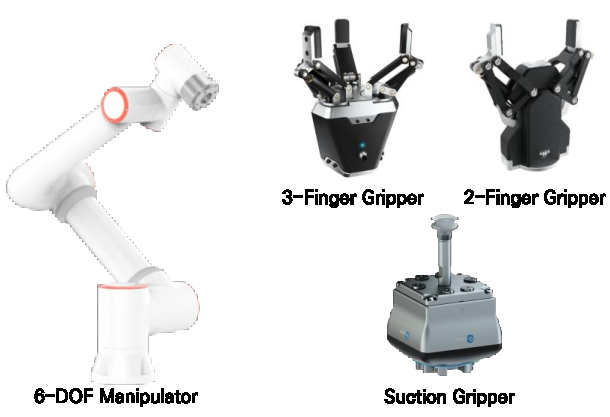
\includegraphics[width=0.38\textwidth]{figures/figure7a.pdf}}
\hfil
\subfloat[\label{fig:fig.7b}]{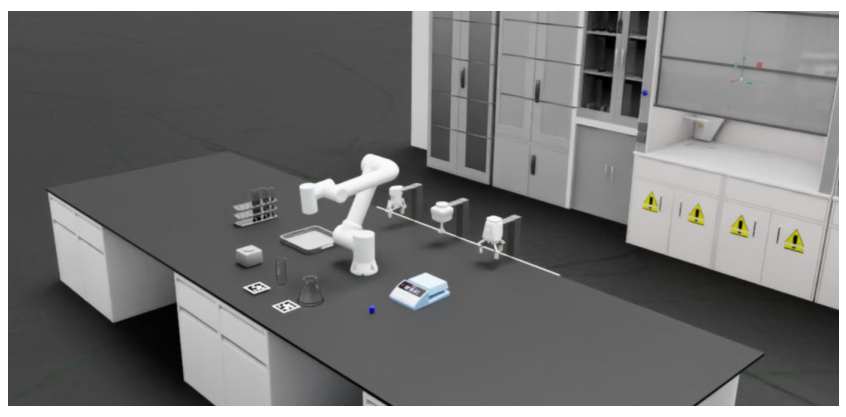
\includegraphics[width=0.525\textwidth]{figures/figure7b.pdf}}
\caption{Hardware components and simulation environment for experimental evaluation. (a) The 6-DoF collaborative manipulator (\textit{FAIRINO-FR5}) alongside three specialized end-effectors: the 2-finger gripper, 3-finger gripper, and suction gripper. (b) The simulation testbed is constructed using \textit{NVIDIA Isaac Sim}. \rev{Physical validation (Section~\ref{sec:4.6}) uses the FR5 with the 2-finger gripper, two RGB cameras, and an electronic scale.}}\label{fig:fig.7}
\end{figure*}

When rearrangement is required, an auxiliary Pick-MoveHolding-Place sequence is inserted before the main procedure, with a tool change to the auxiliary tool performed first if necessary. Rearrangement targets are specified only at the level of a target workspace grid by the Action Reasoner, while precise placement is determined by cuTAMP through collision checking. The target zone is selected to reflect the context of the subsequent procedure, thereby reducing unnecessary rearrangement in later steps and improving overall execution efficiency. The stage-wise world-state update before and after each procedure ensures that plans reflect all preceding changes, including object positions, tool configuration, and auxiliary rearrangement outcomes.


\subsection{Skill Library Module and Execution}\label{sec:3.5}
The Skill Library Module is an execution-layer module that instantiates the nominal trajectories generated by the TAMP Module into sensor-feedback-based motion primitives at execution time. Since TAMP considers only geometric constraints and logical sequencing, the Skill Library invokes the appropriate skill mapped to each TAMP operator to handle physical variables not modeled at the planning stage. The module is organized into two categories: manipulation skills and device operation skills.

\subsubsection{Manipulation Skills}\label{sec:3.5.1}
This category comprises two skills: Adaptive Pouring and Automatic Tool Changing. The Adaptive Pouring skill corrects the nominal trajectory of the Pour operator using real-time weight feedback provided by the Perception Module (Section \ref{sec:3.3.3}). Because liquid flow rates are difficult to predict, the nominal trajectory alone cannot achieve precise quantitative transfer; upon reaching the pouring configuration, the wrist angle is therefore dynamically adjusted through a PD controller based on the error between the target and current weight until the target amount is reached.

The Automatic Tool Changing skill completes the tool exchange as a concrete hardware operation: since the TAMP Module plans the exchange solely as a geometric motion to the tool rack, control signals are applied to the electromagnet upon reaching the exchange point and the mechanical latching sequence is executed to complete the physical coupling.


\begin{figure*}[!t]
\centering
\subfloat[\label{fig:fig.8a}]{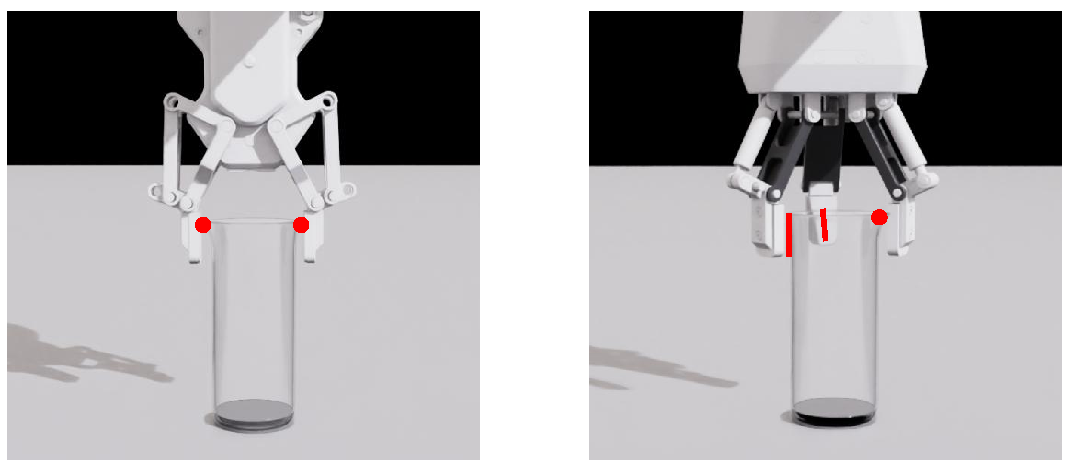
\includegraphics[width=0.4\textwidth]{figures/figure8a.pdf}}
\hfil
\subfloat[\label{fig:fig.8b}]{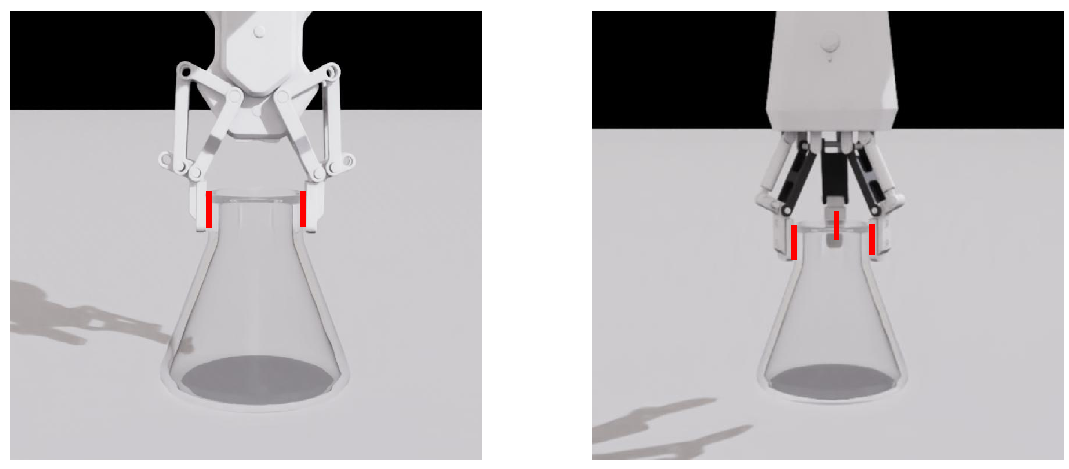
\includegraphics[width=0.4\textwidth]{figures/figure8b.pdf}}
\\
\subfloat[\label{fig:fig.8c}]{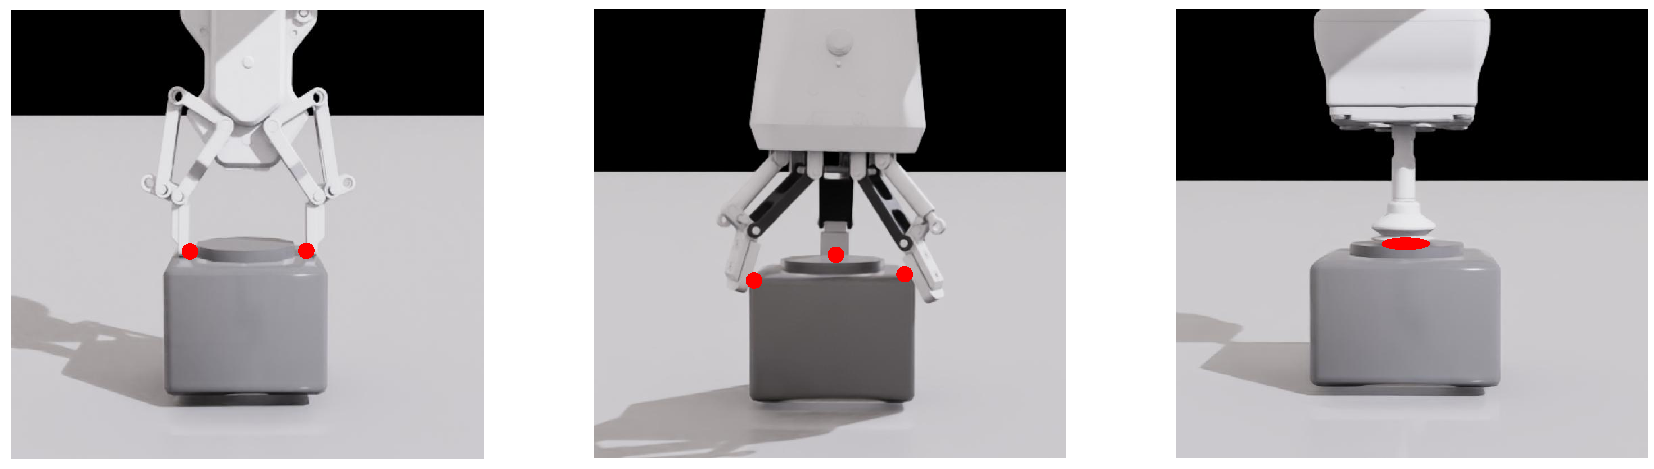
\includegraphics[width=0.62\textwidth]{figures/figure8c.pdf}}
\caption{Motivation for multi-gripper tool selection. The 2-finger gripper provides insufficient contact area on the rim of cylindrical vessels, whereas the 3-finger gripper achieves stable top-down grasping.
For large flat-surface objects exceeding the graspable width of finger grippers, the suction gripper is required. (a) Beaker, (b) Flask, (c) Large flat-surface object.}
\label{fig:fig.8}
\end{figure*}

\subsubsection{Device Operation Skills}\label{sec:3.5.2}
Device operation skills translate device commands, which TAMP treats as abstract symbols, into actual communication protocols and sensor feedback loops; unlike the immediate state transitions assumed by TAMP, physical laboratory devices require time to reach target conditions. This category consists of a single skill, the Feedback-Based Device Control skill.

The Feedback-Based Device Control skill communicates with the corresponding device upon receiving a Heat or Stir command and controls execution until the target physical conditions are met, thereby preventing reaction failures caused by premature progression. Internal sensor values such as temperature or RPM, streamed from the Perception Module (Section \ref{sec:3.3.3}), are continuously monitored, and execution is suspended or locally controlled until the target conditions are met, ensuring that experimental conditions are enforced at the execution layer rather than merely assumed at the planning layer.

\section{Experiments and Evaluation}\label{sec:4}
The proposed framework is simulated with \textit{NVIDIA Isaac Sim} (Fig.~\ref{fig:fig.7}) \rev{and validated on the physical platform (Section~\ref{sec:4.6})} to address the three core limitations identified in Section \ref{sec:2.4}: fixed SDL pipelines that require manual redesign when procedures or apparatus change, unreliable and unpredictable constrained motion planning on low-redundancy manipulators under orientation constraints, and LLM-based planning systems confined to protocol generation without determining the execution context required for each procedure. To validate that all three limitations are addressed, this section evaluates XDL generation accuracy, TAMP planning reliability and latency, LLM-based tool selection and rearrangement reasoning, and end-to-end system performance, proceeding from module-level assessment of individual components to end-to-end evaluation on long-horizon chemical workflows.
\rev{Section~\ref{sec:4.6} then validates the physically deployable subset of the pipeline on the physical manipulator.
All implementation details and hyperparameters required to reproduce the results are given in Section~\ref{sec:4.1.4} and Appendix~A; the project page} at \underline{https://rcilab.github.io/auto\_chem} \rev{hosts demonstration videos and the configuration files}.



\subsection{Experiment Setup}\label{sec:4.1}
This section describes the hardware platform and simulation environment, the chemical tasks selected to span a range of manipulation difficulty, and the fine-tuning procedure for the two LLM components.

\subsubsection{Hardware and Simulation Environments}\label{sec:4.1.1}
The proposed framework is evaluated \rev{in simulation} on a 6-DoF collaborative manipulator (\textit{FAIRINO-FR5}, Fig.~\ref{fig:fig.7}) equipped with three end-effectors to cover the range of object geometries encountered in chemistry laboratory workflows: the 2-finger gripper (\textit{AG95}) for standardized test tubes and small lab assets, the 3-finger gripper (\textit{DH3}) for cylindrical vessels such as beakers and wide-neck flasks, and the suction gripper (\textit{VGC10}) for large flat-surface objects such as container lids and storage boxes. As illustrated in Fig.~\ref{fig:fig.8}, no single gripper configuration can reliably cover all object geometries, motivating the LLM-based dynamic tool assignment described in Section \ref{sec:3.2.3}.

A high-fidelity simulation testbed was developed within \textit{NVIDIA Isaac Sim}, generating 30 distinct initial configurations per task under identical constraint settings to support large-scale randomized trials and controlled ablation. \rev{The TAMP World State is synchronized with simulator-supplied ground-truth object poses and joint configurations at each stage, and the optimized trajectories are streamed back to the simulation for execution; all results in Sections~\ref{sec:4.2}--\ref{sec:4.5} are therefore obtained under externally supplied ground-truth state, and the camera-based perception chain is evaluated on the physical platform in Section~\ref{sec:4.6}.}

\rev{The physical platform used in Section~\ref{sec:4.6} consists of the FR5 with the 2-finger gripper mounted, two calibrated RGB cameras (\nd{Intel RealSense D435, 1280$\times$720, 30\,Hz}) observing the workspace from two sides, an electronic scale (\nd{A\&D EK-610i, 600\,g $\times$ 0.01\,g, RS-232 stream at 10\,Hz}) under the target vessel, and a workspace laid out with the same 12-grid geometry as the simulation.}

\begin{table*}[t]
\begin{minipage}[t]{0.46\textwidth}
\centering
\revbox{%
\centering
\caption{Field-level accuracy of the XDL Generator against reference protocols on 100 test instructions (30\% single-step, 40\% two-step, 30\% three-step), compared after canonicalization.}
\label{tab:xdl_generation}
\begin{tabular*}{\linewidth}{@{\extracolsep{\fill}}lc@{}}
\toprule
\textbf{Field} & \textbf{Exact Match} \\
\midrule
Operator sequence & \nd{100/100}\\
Vessel identities & \nd{100/100}\\
Numerical values and units & \nd{100/100}\\
Procedural ordering & \nd{100/100}\\
\midrule
\textbf{Entire program} & \nd{\textbf{100/100}}\\
\bottomrule
\end{tabular*}}
\end{minipage}\hfill
\begin{minipage}[t]{0.50\textwidth}
\centering
\caption{XDL Validator Classification Accuracy. The benchmark set comprises 20 valid and 80 invalid samples, each evaluated once per error category across the three-layer validation structure.}\label{tab:xdl_validator_cm}
\setlength{\tabcolsep}{3pt}
\begin{tabular*}{\linewidth}{@{\extracolsep{\fill}}lcc@{}}
\toprule
 & \makecell{Validator: Pass \\ (Positive)} & \makecell{Validator: Fail \\ (Negative)} \\
\midrule
Valid & TP = 20 & FN = 0 \\
Invalid & FP = 0 & TN = 80 \\
\bottomrule
\end{tabular*}
\end{minipage}
\end{table*}

\begin{table*}[!t]
\centering
\caption{Classification of Injected XDL Errors for Validator Benchmarking.}\label{tab:xdl_injected_errors}
\begin{tabular}{@{}p{0.15\dimexpr\linewidth-8\tabcolsep\relax}p{0.175\dimexpr\linewidth-8\tabcolsep\relax}p{0.2\dimexpr\linewidth-8\tabcolsep\relax}p{0.275\dimexpr\linewidth-8\tabcolsep\relax}p{0.2\dimexpr\linewidth-8\tabcolsep\relax}@{}}
\toprule
Validation Layer & Error Category & Error Condition & Injected XDL Example & Remarks \\
\midrule
Syntax & Missing required attribute & Intentional omission of mandatory attributes & \texttt{<Transfer to\_vessel="flask\_A" volume="10 mL" />} & from\_vessel \newline missing \\
\addlinespace
Syntax & Undefined tag / attribute name & Use of disallowed tag or attribute name & \texttt{<Move object="flask\_A" to\_vessel="flask\_B" />} & Using to\_vessel \newline instead of place \newline in Move \\
\addlinespace
Object \newline existence & Non-existent object reference & Reference to object absent from workspace & \texttt{<Stir vessel="flask\_C" time="30 s" />} & flask\_C \newline not registered \newline in workspace \\
\addlinespace
Physical \newline feasibility & Physically \newline infeasible sequence & Physical operation on an empty container & \texttt{<Stir vessel="beaker\_A" time="1 min" />} & Stirring \newline empty \newline beaker\_A \\
\bottomrule
\end{tabular}
\end{table*}

\subsubsection{Chemical Experiments}\label{sec:4.1.2}
Three manipulation tasks are selected to cover the essential procedures of real-world chemical experiments while spanning a range of planning complexity and manipulation difficulty. Move represents pick-and-place of laboratory objects and is evaluated using large-radius objects that require the suction gripper to assess the LLM's tool selection capability and manipulation success rate. Transfer represents liquid handling, a fundamental procedure in chemical synthesis, and tests the system's ability to maintain spill-free orientation constraints throughout the transit phase while tilting the source container and pouring its contents into a target vessel. Stir is chosen over simpler device operations such as heating because it demands higher spatial precision: the robot must relocate the vessel onto a magnetic stirrer and precisely insert a magnetic stir bar into the narrow opening, making it an ideal scenario for evaluating complex, multi-step task and motion planning.

\subsubsection{LLM Fine-Tuning and Training Details}\label{sec:4.1.3}
The two LLM components introduced in Section \ref{sec:3.2}, the XDL Generator and the Action Reasoner, are each fine-tuned on a domain-specific dataset constructed to reflect the combinatorial structure of the target task. For the XDL Generator, the training dataset is constructed at a scale of 5,000 samples across four combinatorial axes: synonym variations for each of the six core XDL operators (Add, Stir, HeatChill, Transfer, CleanVessel, Move), continuous numerical parameter ranges (0--20 mL for volume, 0--20$^\circ$C for temperature, 1--30 s for time), four instance identifiers per vessel type yielding 16 unique object identifiers, and command complexity ranging from single-operator instructions to three-step composite procedures with a weighted distribution of 30\% single-step, 40\% two-step, and 30\% three-step. Since the task constitutes a structural mapping to a fixed XDL schema, the output space is inherently constrained and this dataset covers the principal combinatorial patterns, as supported by the results in Section \ref{sec:4.2.1}. Training is performed by applying LoRA (rank $r = 16$, $\alpha = 32$, dropout 0.05) to a 4-bit quantized \textit{Llama 3.2 1B} model, using an 8-bit AdamW optimizer with a learning rate of $2 \times 10^{-4}$, an effective batch size of 16, and 5 epochs.
\rev{Training, validation, and test instructions are separated at every level of the combinatorial construction.
\nd{The paraphrase templates of each operator are partitioned 70/10/20 into training, validation, and test, so that no test instruction shares a template with training; the fourth instance identifier of each vessel type appears only in the test set; 6 of the 36 ordered operator pairs (repeats included) and 10 of the three-step compositions are held out for testing; and test values of volume, temperature, and time are drawn from the same ranges but are disjoint from every value used in training.}
Test instructions additionally embed the operators in longer sentences with distractor clauses that do not occur in training.}



For the Action Reasoner, the training dataset consists of 3,000 samples generated combinatorially by placing up to four objects on 12 workspace grids. For each combination of the six XDL operators, rearrangement necessity is determined according to task-specific blocking criteria, and the ground-truth destination is assigned as either a context-aware target zone or a workspace edge depending on whether the obstacle is the target of the subsequent procedure. Candidate workspace grids are provided as input features after excluding fixed equipment and occupied grids, categorized solely by locational characteristics to prevent label leakage. The dataset is balanced across rearrangement-required and rearrangement-unnecessary cases, as well as context-aware and irrelevant obstacle cases, to prevent over-prediction of rearrangement. Training follows the same \textit{Llama 3.2 1B} base model with LoRA configured at rank $r = 8$, $\alpha = 16$, dropout 0.05, a learning rate of $1 \times 10^{-4}$, batch size 16, and 3 epochs. The differing LoRA configurations were selected empirically based on validation performance, rather than through a dedicated hyperparameter ablation.



\subsubsection{Implementation Details and Reproducibility}\label{sec:4.1.4}
\rev{All settings required to reproduce the results are summarized here and listed exhaustively in Appendix~A.
The simulation runs in \textit{NVIDIA Isaac Sim} \nd{4.2.0} with PhysX at \nd{1/60\,s} and \nd{4} solver substeps.
The workspace is a \nd{0.9\,m $\times$ 0.6\,m} table of which a \nd{0.6\,m $\times$ 0.45\,m} region is discretized into 12 grids of \nd{0.15\,m $\times$ 0.15\,m} arranged \nd{4 $\times$ 3}, the remainder holding the tool rack and fixed devices.
Each trial randomizes object positions uniformly within \nd{$\pm$5\,cm} of the grid centre, object yaw within \nd{$\pm$180$^\circ$}, and the robot initial configuration within \nd{$\pm$10$^\circ$} of its home pose, using fixed seeds 0--29 per task that are shared by both planners.
Non-target obstacle primitives are enlarged by \nd{10\,mm}; target primitives are not enlarged.
The simulated FR5 is driven by \nd{joint-position control at 60\,Hz} and the physical FR5 through \nd{the vendor servo interface at 125\,Hz}, both with joint velocity and acceleration limits of \nd{180$^\circ$/s and 360$^\circ$/s$^2$}.}

\rev{The simulator represents rigid-body contact and grasp friction, joint-space trajectory-tracking error, and the randomized initial states; it does not represent fluid dynamics, scale latency or noise, or gripper compliance under load, which are characterized on the physical platform in Section~\ref{sec:4.6}.
Planning success is defined as a trajectory returned within the time budget that satisfies all constraints at every evaluated point.
A simulated trial is counted as an execution success only if (i) no contact is reported between the robot or the grasped object and any non-target object, (ii) the grasped object remains within \nd{5\,mm} of its grasp-frame pose throughout, (iii) the upright constraint holds at every control step, and (iv) the terminal condition of the operator is met: final placement within \nd{10\,mm} and \nd{5$^\circ$} of the target for Move, the pour configuration reached above the target vessel for Transfer, and the stir bar inside the vessel for Stir.}

\rev{The planner comparison of Section~\ref{sec:4.3} is a system-level wall-clock comparison of the two planners in their deployment configurations on one workstation (\nd{Intel Core i9-13900K, NVIDIA RTX 4090, 64\,GB RAM}), not a compute-normalized comparison: cuTAMP runs its batched optimization on the GPU with 1,024 particles, 1,000 optimization steps, \nd{Adam at a learning rate of $10^{-2}$}, cost weights \nd{$w_{\mathrm{coll}}=10$, $w_{\mathrm{up}}=5$, $w_{\mathrm{goal}}=1$}, collision cost evaluated at \nd{32} interpolated points per segment, and three re-initializations on failure, whereas our PDDLStream implementation (\nd{the public reference implementation with FastDownward and the adaptive algorithm}) executes its streams on a single CPU thread.
Its streams are a grasp sampler (\nd{25 candidate grasps per object}), a placement sampler (\nd{uniform over the target grid}), an inverse-kinematics stream (\nd{numerical IK, 10 attempts per grasp--placement pair}) that rejects configurations violating the upright constraint, and a motion stream (\nd{RRT-Connect with 50 restarts}), with \nd{unlimited stream re-instantiation} within the 60\,s budget.
Baseline sampler counts were tuned to maximize baseline success on \nd{10 tuning configurations (seeds 100--109) disjoint from the evaluation configurations}; the selected values are those beyond which further increases did not change the success rate within the budget.}

\subsection{XDL Generation Evaluation}\label{sec:4.2}
This section evaluates the XDL generation pipeline across two aspects: the accuracy of the XDL Generator in converting natural language commands into valid protocols, and the ability of the XDL Validator to detect and intercept physically invalid protocols before execution.

\subsubsection{Language Command to XDL Format}\label{sec:4.2.1}
To assess whether the XDL Generator reliably converts natural language commands into \rev{correct} protocols across varying task complexities, 100 test instructions spanning single-step to three-step composite workflows were evaluated.
The test instructions were distributed across 30\% single-step, 40\% two-step, and 30\% three-step procedures, and were constructed to include randomized synonym combinations and complex sentence structures beyond isolated commands.
\rev{Generator accuracy is measured against a reference XDL protocol for each instruction, \nd{written by one author before any model output was inspected and independently re-annotated on a random 30\% subset by a second author with full agreement}.
Generated and reference protocols are compared field by field after canonicalization: vessel identifiers are case-folded, volumes are expressed in mL, temperatures in $^\circ$C, and times in s, and attribute types are checked against the XDL schema.
As summarized in Table~\ref{tab:xdl_generation}, the generated operator sequence, vessel identities, numerical values, and procedural ordering match the reference in \nd{100} of 100 instructions, and the entire program matches exactly in \nd{100} of 100; no syntax error or semantic tag confusion was observed in any test case.
Three of the 100 instructions contain a contradiction, in which a subsequent operator requires a vessel state already invalidated by a preceding operation; the generator transcribed these faithfully, so they count as generator successes, and their rejection by the validator is reported separately in Section~\ref{sec:4.2.2}.}
The average inference time per command was 1.57\rev{\,s}, confirming that the module introduces negligible latency relative to the overall pipeline execution time.



\begin{table*}[t]
\revbox{%
\caption{Comparison of planning success and latency between sequential parameter-binding (PDDLStream) and batched joint optimization-based (cuTAMP) TAMP solvers on the 6-DoF \textit{FR5} manipulator under simulator-supplied ground-truth state, over 30 paired randomized initial configurations per task with a 60\,s budget. Success is given with the Wilson 95\% confidence interval and the exact McNemar $p$-value on the paired configurations. Latency is the mean $\pm$ std over successful trials; the restricted mean time-to-solution (RMTS) treats timed-out and early-terminated trials as right-censored at 60\,s. The last column is cuTAMP success when the World State is perturbed with perception residuals resampled from the physical measurements of Section~\ref{sec:4.6.1}.}
\label{tab:tamp_comparison}
\centering
\footnotesize
\setlength{\tabcolsep}{3pt}
\begin{tabular*}{\linewidth}{@{\extracolsep{\fill}}llccccccc@{}}
\toprule
Task & Solver & \makecell{Success (\%)\\{}[95\% CI]} & \makecell{McNemar\\$p$} & \makecell{Latency,\\successes (s)} & \makecell{RMTS\\(s)} & \makecell{Timeout\\(\%)} & \makecell{Early\\term. (\%)} & \makecell{Success,\\percep. noise (\%)} \\
\midrule
\multirow{2}{*}{Transfer}
 & PDDLStream & 66.7 [48.8, 80.8] & \multirow{2}{*}{$2.0\times10^{-3}$} & $7.21 \pm 10.26$ & 24.8 & 10.0 & 20.0 & -- \\
 & cuTAMP     & 100.0 [88.6, 100.0] & & $31.18 \pm 1.44$ & 31.2 & 0.0  & 0.0 & \nd{100.0} \\
\midrule
\multirow{2}{*}{Move}
 & PDDLStream & 83.3 [66.4, 92.7] & \multirow{2}{*}{$0.063$} & $0.17 \pm 0.12$ & 10.1 & 0.0  & 16.7 & -- \\
 & cuTAMP     & 100.0 [88.6, 100.0] & & $17.60 \pm 3.55$ & 17.6 & 0.0 & 0.0 & \nd{100.0} \\
\midrule
\multirow{2}{*}{Stir}
 & PDDLStream & 60.0 [42.3, 75.4] & \multirow{2}{*}{$4.9\times10^{-4}$} & $0.79 \pm 0.70$ & 24.5 & 23.3 & 13.3 & -- \\
 & cuTAMP     & 100.0 [88.6, 100.0] & & $28.83 \pm 1.00$ & 28.8 & 0.0 & 0.0 & \nd{96.7} \\
\bottomrule
\end{tabular*}}
\end{table*}



\subsubsection{XDL Validator}\label{sec:4.2.2}
\rev{To verify that the XDL Validator intercepts the failure classes it is designed for, a benchmark test was conducted by injecting anomalous data across four error categories: missing required attribute, undefined tag or attribute, non-existent object reference, and symbolic state-precondition violation.}
The three contradictory instructions of Section~\ref{sec:4.2.1} confirm that the validator intercepts errors arising from user instruction contradictions, \rev{and the benchmark extends this check to the remaining tested classes}.
On this benchmark, the XDL Validator achieves 100\% classification accuracy, with zero false positives and zero false negatives; the resulting confusion matrix in Table \ref{tab:xdl_validator_cm} confirms that the validator intercepts all injected errors \rev{of the tested classes, with a per-class recall of \nd{20/20} for each class}.
The composition of the benchmark set is summarized in Table \ref{tab:xdl_injected_errors}.
In each case, the system returned a targeted error message such as ``Cannot Stir empty vessel: beaker\_A,'' enabling the user to revise the instruction before any robot motion occurred.
\rev{These figures characterize the tested syntactic, object-existence, and state-precondition classes only; conditions outside the benchmark, such as vessel capacity, chemical incompatibility, and contamination constraints, are discussed in Section~\ref{sec:5.3}.
\nd{The physical-feasibility layer additionally enforces two symbolic checks that require no chemical knowledge, vessel capacity and device placement, and the benchmark was extended to 20 valid and 120 invalid samples across six error classes with unchanged zero false positives and zero false negatives.}
To probe the containment of language-model errors beyond the benchmark, \nd{70 adversarial instructions in seven categories of 10 (out-of-schema operations, fictitious vessels, existing but wrong targets, out-of-range volumes and temperatures, conflicting long sequences, prompt-injection phrasing embedded in valid commands, and ambiguous but grammatically valid commands) were submitted to the pipeline; the 60 instructions in the six invalid categories were all intercepted at the validator with the correct error class, and the 10 ambiguous-but-valid commands passed validation, as expected, and constitute the residual exposure discussed in Section~\ref{sec:5.3}}.}


\begin{figure}[!t]
\centering
\revbox{%
\fbox{\parbox[c][0.6\linewidth][c]{\dimexpr\linewidth-2\fboxsep-2\fboxrule\relax}{\centering\nd{Figure placeholder: Kaplan--Meier solved fraction versus wall-clock planning time for PDDLStream and cuTAMP on Transfer, Move, and Stir (30 paired configurations each, 60\,s budget), generated from the planning logs.}}}
\caption{Solved fraction as a function of wall-clock planning time (Kaplan--Meier estimate) for the two planners on each task, with timed-out and early-terminated trials right-censored at the 60\,s budget. \nd{PDDLStream solves its easy instances within seconds and plateaus below 100\%, whereas cuTAMP solves every instance within a band of 29--34\,s.}}
\label{fig:km}}
\end{figure}

\subsection{TAMP Planning Reliability and Latency Evaluation}\label{sec:4.3}
This section evaluates the ability of the TAMP Module to achieve reliable planning success rates and predictable termination time under orientation constraints on low-redundancy manipulators, addressing the structural limitation of sequential parameter-binding approaches identified in Section \ref{sec:2.2}. The proposed planning module is compared against PDDLStream as a representative sequential parameter-binding baseline across three chemical tasks, with 30 randomized initial configurations per task under identical starting poses, target conditions, and orientation constraints for spillage prevention, and a time budget of 60 seconds per trial. The proposed planning module was configured with 1,024 parallel particles and 1,000 optimization steps per planning attempt.
The reported metrics reflect algorithmic planning latency exclusively, excluding physical execution and simulation rendering times.
\rev{The full configuration of both planners and the tuning procedure for the baseline are given in Section~\ref{sec:4.1.4} and Appendix~A; as stated there, the comparison is a system-level wall-clock comparison of the two planners in their deployment configurations on one workstation, not a compute-normalized comparison.}

The proposed planning module achieves higher planning success rates than the sequential parameter-binding baseline across all three tasks, with the most pronounced improvement on the Transfer task where orientation constraints are most restrictive, recording 100.0\% versus 66.7\% on the same 6-DoF manipulator\rev{; the difference is significant on the paired configurations for Transfer ($p = 2.0\times10^{-3}$, exact McNemar) and Stir ($p = 4.9\times10^{-4}$), whereas on Move, where the baseline already succeeds on 83.3\% of configurations, it is not significant at this sample size ($p = 0.063$)}.
Beyond success rate, the proposed planning module \rev{returns every plan within a bounded band of termination times}, a property that sequential parameter-binding approaches cannot guarantee.
These results are summarized in Table \ref{tab:tamp_comparison} \rev{and Fig.~\ref{fig:km}}.


\begin{table*}[t]
\centering
\caption{LLM-based tool selection and corresponding task performance. Each task--tool condition is evaluated on 30 unseen test scenarios not present in the fine-tuning dataset, for a total of 120 trials. \rev{Bottle and box are object classes absent from fine-tuning; beaker, flask, and tube occur in fine-tuning with different identifiers and layouts.}}
\label{tab:tool_selection}
\begin{tabular*}{\linewidth}{@{\extracolsep{\fill}}lllc@{}}
\toprule
\textbf{Task} & \textbf{Selected Tool} & \textbf{Target Object} & \textbf{Success Rate (\%)} \\ \midrule
\multirow{2}{*}{Move} & 3-finger gripper & Beaker, Flask, Tube & 100.0 \\
 & suction gripper & Bottle, Box & 96.67 \\ \midrule
Transfer & 2-finger gripper & Beaker, Flask, Tube & 100.0 \\ \midrule
Stir & 3-finger gripper & Beaker, Flask, Tube & 93.33 \\ \bottomrule
\end{tabular*}
\end{table*}


On the Transfer task, the proposed planning module achieves 100.0\% success by jointly optimizing 1,024 candidate particles in parallel toward the constraint manifold, enabling effective exploration of the feasible region even when kinematic redundancy is limited. PDDLStream, by contrast, achieves only 66.7\%: 10.0\% of trials time out because its sequential sampling mechanism depends heavily on whether early random configurations happen to satisfy the orientation constraint, and the remaining 20.0\% terminate early \rev{\nd{because the adaptive algorithm reaches its maximum stream-complexity level without a feasible binding}, a failure that occurs before the budget is exhausted and therefore does not depend on the time budget}. On the Move task, the lower constraint complexity of top-grasp-based manipulation allows PDDLStream to reach 83.3\%, whereas the proposed planning module eliminates the remaining failures and achieves 100.0\%. On the Stir task, the requirement for precise stir-bar insertion into narrow vessel openings imposes tight spatial constraints that reduce PDDLStream to 60.0\%, with 23.3\% timeouts and 13.3\% early terminations, while the proposed planning module maintains 100.0\% success. Across all three tasks, these results show that batched joint differentiable optimization handles orientation and spatial constraints more reliably than sequential parameter binding on low-redundancy manipulators.
\rev{\nd{A cuTAMP ablation with 256 particles, which reduces the GPU work fourfold, still attains 100\% success on all three tasks within the budget, indicating that the advantage does not rest on the particle budget alone.}
Perturbing the World State with perception residuals resampled from the physical measurements of Section~\ref{sec:4.6.1} leaves cuTAMP success at \nd{100.0\%, 100.0\%, and 96.7\%} on Transfer, Move, and Stir (last column of Table~\ref{tab:tamp_comparison}), within one trial of the ground-truth condition.}

The two approaches also differ in temporal predictability\rev{, and this difference concerns the distribution of termination times rather than mean speed}.
\rev{Timed-out and early-terminated trials are unsolved within the budget and are treated as right-censored at 60\,s; Fig.~\ref{fig:km} plots the resulting Kaplan--Meier solved fraction against wall-clock time, and Table~\ref{tab:tamp_comparison} reports the restricted mean time-to-solution over the budget alongside the conditional latency of successful trials.
PDDLStream is faster when it succeeds ($7.21 \pm 10.26$\,s against $31.18 \pm 1.44$\,s on Transfer) and accordingly has the lower restricted mean on every task, but its solved fraction plateaus at 66.7\%, 83.3\%, and 60.0\% with a tail that ends in timeouts, so the time at which a valid plan is obtained is unpredictable for a given configuration.
The proposed planning module solves every configuration, and the time at which it does so lies within a band of \nd{29--34\,s} on Transfer by construction of the fixed particle and step budget; its nonzero standard deviation reflects variation among successful solutions rather than a mixture of successes and unresolved failures.}
Overall, unlike PDDLStream, the proposed planning module consistently terminates within a bounded time envelope while returning a valid solution, a property that is critical for time-sensitive chemical workflows in which unpredictable planning delays may compromise reaction conditions.



\subsection{LLM-based Tool Selection and Rearrangement Action Reasoning}\label{sec:4.4}
To verify that the LLM Module reliably performs its two core functions, namely semantic tool assignment and context-aware obstacle rearrangement, the module is evaluated on unseen test scenarios not present in the fine-tuning dataset. The evaluation is structured as a two-stage ablation, because both functions are exercised within a single action sequence and removing the module entirely would make it difficult to distinguish their individual contributions. Section \ref{sec:4.4.1} isolates tool assignment by evaluating inference accuracy on unseen scenarios independently of rearrangement. Section \ref{sec:4.4.2}, in contrast, isolates the rearrangement strategy by holding tool selection constant and comparing context-aware placement against no-rearrangement and random-rearrangement baselines. Section \ref{sec:4.5} then verifies that the two functions combine effectively in the integrated pipeline through end-to-end evaluation.

\subsubsection{Semantic Tool Assignment and Action Reasoner Evaluation}\label{sec:4.4.1}
To assess whether the LLM Module assigns appropriate end-effectors across diverse task--object combinations, including object types not encountered during fine-tuning, tool selection accuracy is evaluated on 120 unseen test scenarios, comprising 30 trials per task--tool condition.
\rev{Relative to the 3,000 fine-tuning samples, the test scenarios are unseen at three levels: \nd{the bottle and box classes, which require the suction gripper, do not occur in fine-tuning; a test layout counts as unseen only if its occupancy pattern, i.e., the set of occupied grids together with the object class in each, does not occur in training, and relabelling object identifiers on a training pattern does not qualify; and 4 of the 36 ordered current/next operator pairs, repeats included, are held out entirely}.} As summarized in Table \ref{tab:tool_selection}, the module achieves 100\% accuracy for Move with the 3-finger gripper and Transfer with the 2-finger gripper, 96.67\% for Move with the suction gripper, and 93.33\% for Stir with the 3-finger gripper. The model consistently assigns the 3-finger gripper for cylindrical vessels across Move and Stir tasks, the 2-finger gripper for Transfer to enable side-grasp pouring, and the suction gripper for flat-surface objects that exceed the graspable width of finger-based end-effectors. The average inference time of 0.0665\,s confirms that tool selection introduces negligible latency into the overall pipeline.

These results also reveal that no single fixed end-effector can cover the full set of evaluated task--object combinations. The 2-finger gripper cannot grasp large objects due to grip width constraints; the 3-finger gripper cannot execute the side-grasp-based pouring required for Transfer; and the suction gripper cannot achieve the stable insertion necessary for Stir. The tool selection accuracy reported above therefore validates not only the module's inference quality but also the architectural decision to support dynamic tool assignment as a prerequisite for operational coverage.

Beyond tool selection, the comprehensive reasoning capability of the Action Reasoner is evaluated on 600 unseen scenarios covering all four inference outputs: main tool, rearrangement necessity, auxiliary tool, and destination grid. As summarized in Table \ref{tab:action_reasoner}, main tool, rearrangement necessity, and auxiliary tool selection each achieve 100.0\% accuracy. For the destination grid, category-level accuracy reaches 100.0\%, while the exact grid match rate within a category is 76.5\%. The Action Reasoner selects a single target workspace grid to specify the destination work zone, while precise placement coordinates within that zone are determined by the TAMP Module through collision checking in continuous space (Section \ref{sec:3.2.3}). The category-level accuracy of 100.0\% therefore confirms that the module fulfills this role in every scenario. The lower exact grid match rate reflects the fact that multiple grids within the same category can serve as valid placement candidates; since the final coordinate is resolved by the TAMP Module, this discrepancy does not affect downstream planning performance.

\begin{table}[t]
\centering
\caption{Action Reasoner inference accuracy on unseen test scenarios. Evaluated on 600 unseen scenarios covering all four inference outputs across task--object combinations not present in the fine-tuning dataset.}\label{tab:action_reasoner}
\begin{tabular*}{\linewidth}{@{\extracolsep{\fill}}lc@{}}
\toprule
Metric & Accuracy (\%) \\
\midrule
Main Tool & 100.0 \\
Need Rearrange & 100.0 \\
Rearrangement Tool & 100.0 \\
Target Grid (category) & 100.0 \\
Target Grid (exact) & 76.5 \\
\bottomrule
\end{tabular*}
\end{table}

\begin{table*}[!t]
\centering
\caption{TAMP success rates and sequence completion rates by rearrangement strategy. Each sequence-condition pair is evaluated over 30 randomized trials \rev{under simulator-supplied ground-truth state; the lower two sequences are the three-step workflows of Table~\ref{tab:end_to_end}}.}\label{tab:rearrange_eval}
\begin{tabular*}{\linewidth}{@{\extracolsep{\fill}}llccc@{}}
\toprule
Sequence & Metric & No Rearrange & Random Rearrange & Context-Aware \\
\midrule
\multirow{2}{*}{Transfer $\rightarrow$ Stir} & Step 1 Success (\%) & 0.0 & 60.0 & 96.67 \\
 & Sequence Completion (\%) & 0.0 & 50.0 & 96.67 \\
\addlinespace
\multirow{2}{*}{Stir $\rightarrow$ Transfer} & Step 1 Success (\%) & 100.0 & 100.0 & 100.0 \\
 & Sequence Completion (\%) & 13.33 & 40.0 & 83.33 \\
\addlinespace
\rev{Transfer $\rightarrow$ Stir $\rightarrow$ Move} & \rev{Step 1 Success (\%)} & \rev{\nd{0.0}} & \rev{\nd{60.0}} & \rev{\nd{96.67}} \\
 & \rev{Sequence Completion (\%)} & \rev{\nd{6.67}} & \rev{\nd{36.67}} & \rev{\nd{93.33}} \\
\addlinespace
\rev{Move $\rightarrow$ Transfer $\rightarrow$ Stir} & \rev{Step 1 Success (\%)} & \rev{\nd{100.0}} & \rev{\nd{100.0}} & \rev{\nd{100.0}} \\
 & \rev{Sequence Completion (\%)} & \rev{\nd{13.33}} & \rev{\nd{40.0}} & \rev{\nd{96.67}} \\
\bottomrule
\end{tabular*}
\end{table*}

\begin{figure*}[!t]
\centering
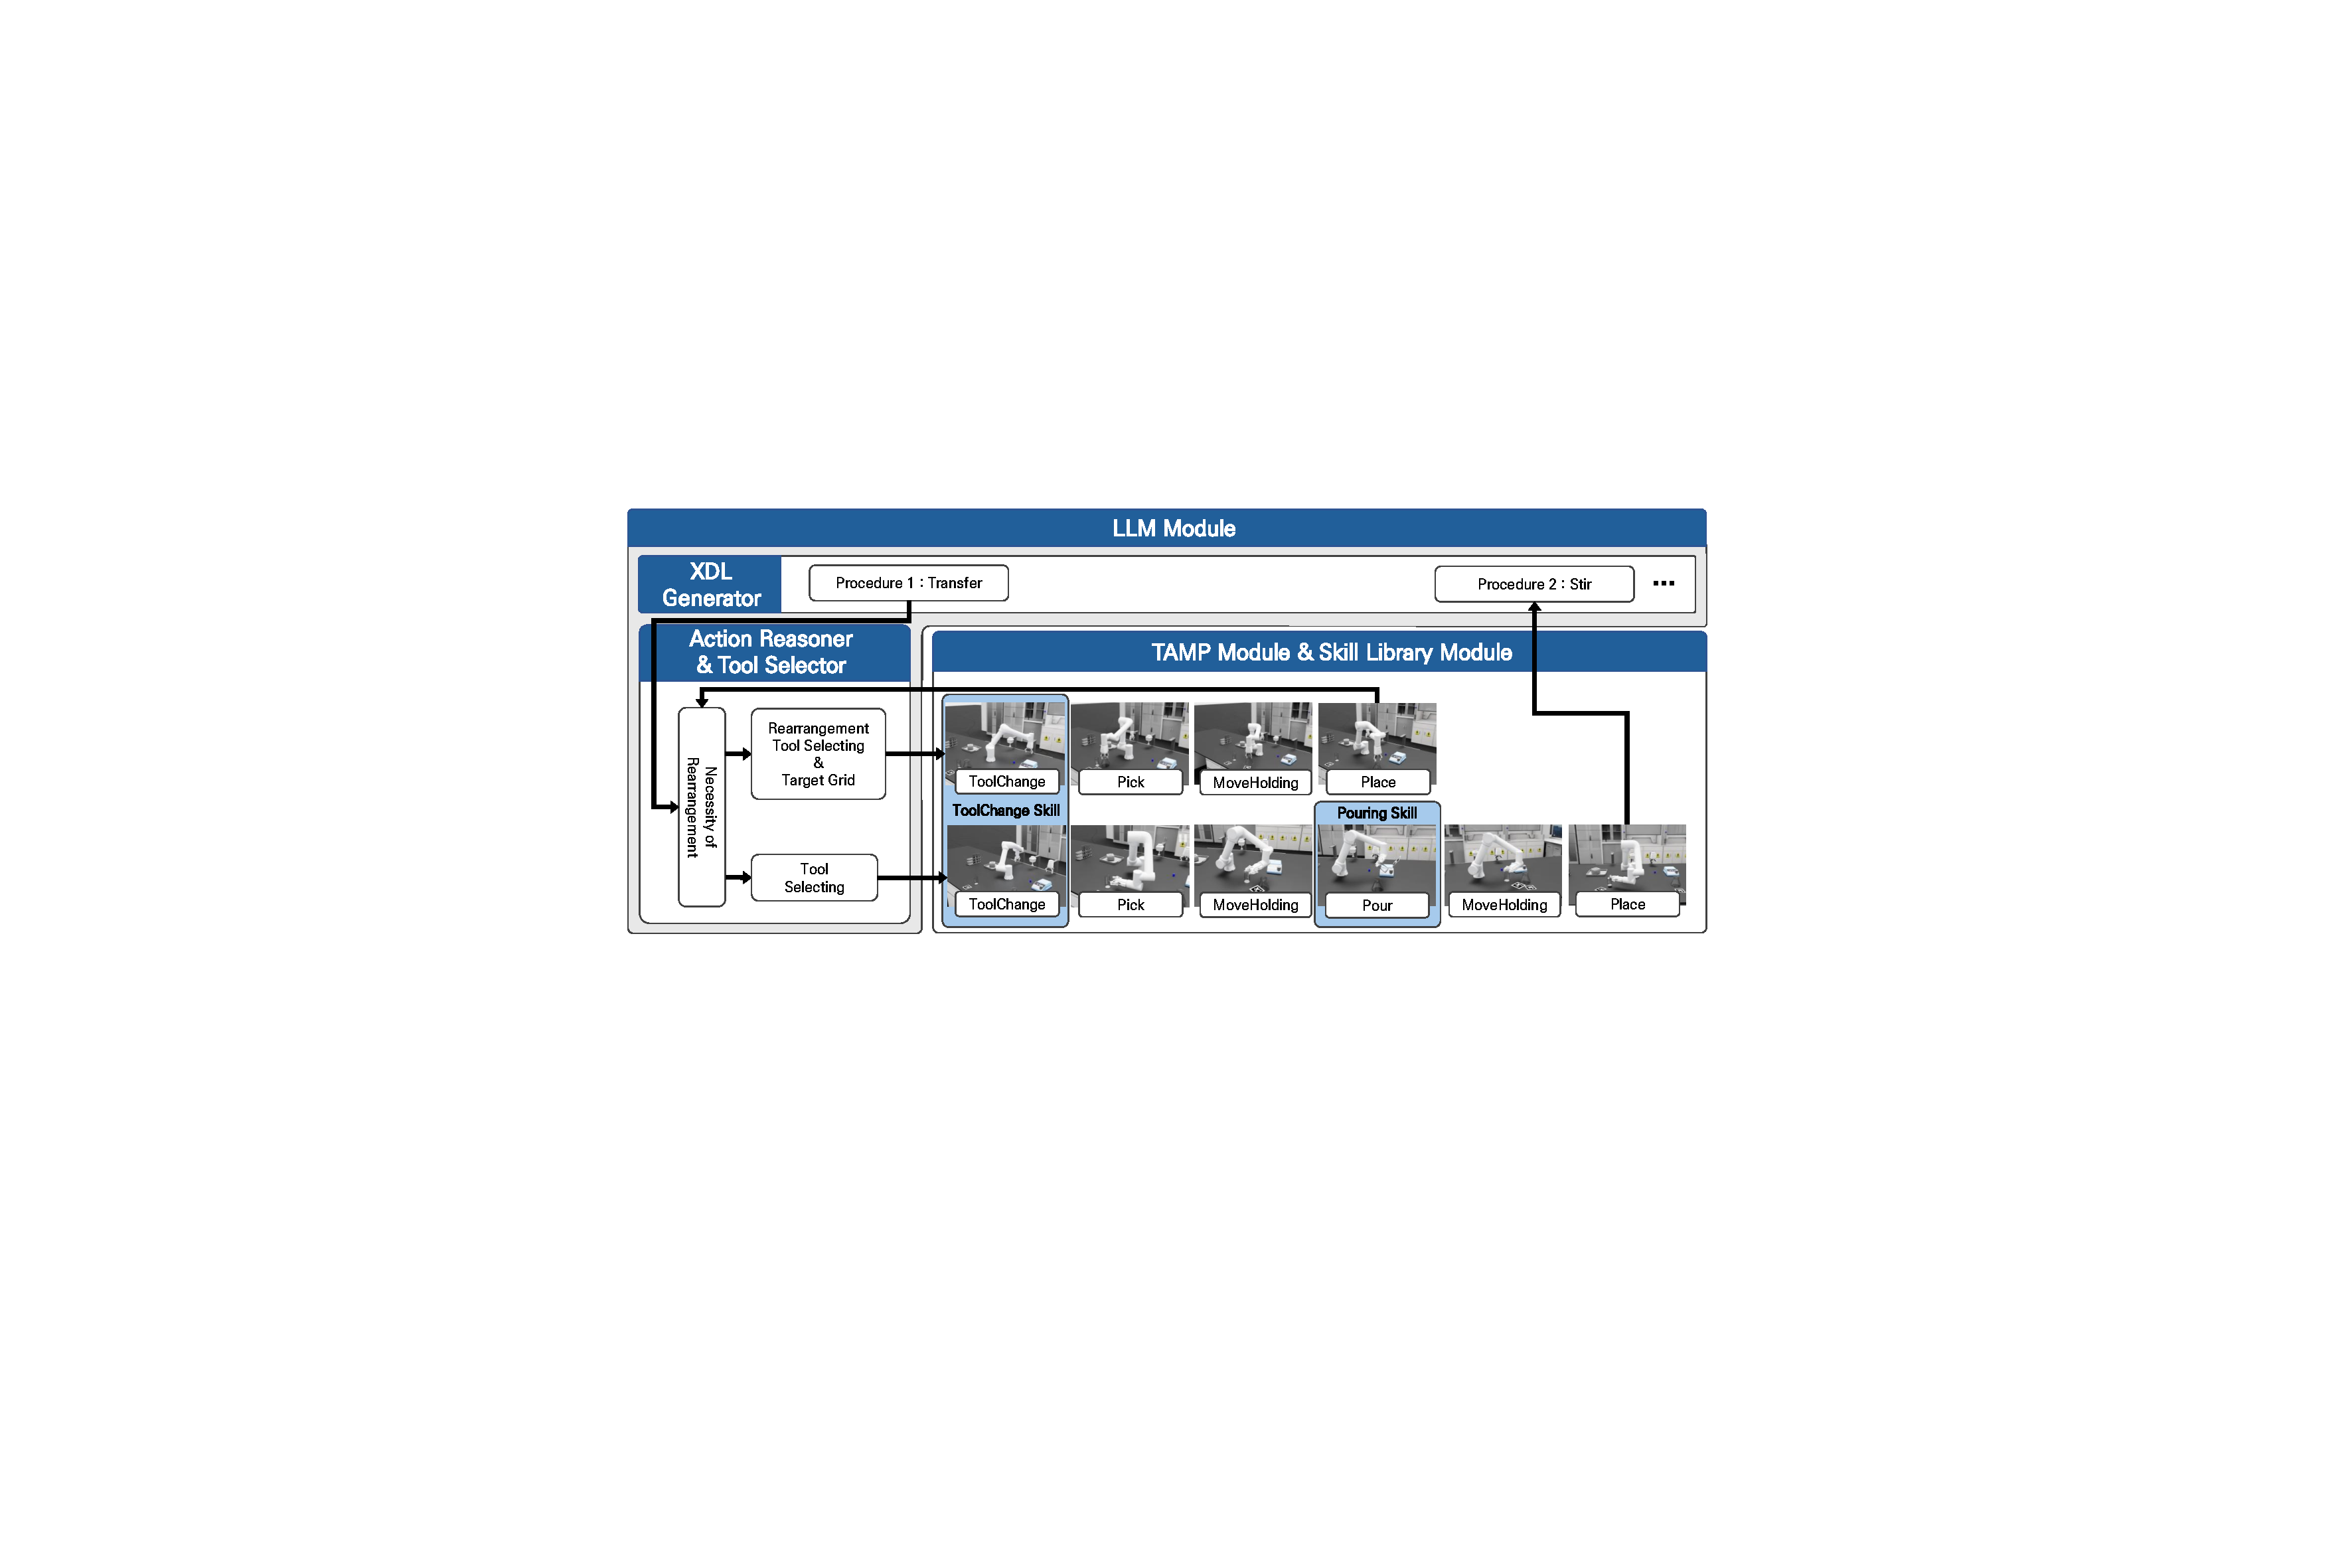
\includegraphics[width=0.95\textwidth]{figures/figure9.pdf}
\caption{Execution flow of the TAMP pipeline for a Transfer procedure. The Action Reasoner determines tool selection and rearrangement necessity. When rearrangement is required, an auxiliary rearrangement sequence (upper path) is inserted prior to the main experimental procedure (lower path), which includes sensor-feedback-based skills such as adaptive pouring.}\label{fig:fig.9}
\end{figure*}

\subsubsection{Context-Aware Rearrangement Strategy Evaluation}\label{sec:4.4.2}
To isolate the contribution of procedural context in rearrangement decisions, three conditions are compared. The No Rearrange condition executes the main task directly even when obstacles block the workspace. The Random Rearrange condition detects obstacles and relocates them to arbitrarily selected unoccupied grids, serving as an ablation that preserves spatial clearance but removes context-awareness. The Context-Aware condition uses the Action Reasoner to analyze the subsequent procedure and preemptively relocate obstacles to the work zone required by the next step. Tool selection is held constant across all three conditions to isolate rearrangement strategy as the sole independent variable.



Table \ref{tab:rearrange_eval} reports the Step~1 TAMP success rate and sequence completion rate for each condition across two evaluation sequences: Transfer $\rightarrow$ Stir, chosen because the wide workspace required by side-grasp pouring makes rearrangement most frequent, and the reverse order Stir $\rightarrow$ Transfer as a control. Context-aware rearrangement achieves the highest sequence completion rate in both cases, reaching 96.67\% and 83.33\%, compared to 50.0\% and 40.0\% for random rearrangement and 0\% and 13.33\% for no rearrangement.

The failure patterns across conditions clarify how context-awareness contributes beyond spatial clearance. Without rearrangement, Step~1 success on Transfer $\rightarrow$ Stir drops to 0\% due to workspace congestion. Random rearrangement recovers Step~1 to 60.0\% by clearing the immediate workspace, but since obstacles are placed without regard to the subsequent procedure, Step~2 encounters new collisions or requires additional rearrangement, limiting sequence completion to 50.0\%. Context-aware rearrangement simultaneously secures workspace for Step~1 and positions obstacles where they will be needed for Step~2, achieving 96.67\% sequence completion while eliminating the redundant manipulations that random placement incurs. \rev{These results show that procedural context, rather than spatial clearance alone, significantly improves sequence completion under the evaluated conditions (\nd{exact McNemar on the paired seeds, $p<0.001$ against random rearrangement}) within the six-operator, 12-grid workspace.
The same comparison on the two three-step workflows of Section~\ref{sec:4.5} (lower half of Table~\ref{tab:rearrange_eval}) yields \nd{93.3\% and 96.7\%} sequence completion with context-aware rearrangement against \nd{36.7\% and 40.0\%} with random rearrangement and \nd{6.7\% and 13.3\%} without, consistent with the two-step results; these figures extend the evidence within the tested domain and are presented as such.}
Fig.~\ref{fig:fig.9} illustrates the resulting execution flow for a representative Transfer procedure, showing how the auxiliary rearrangement sequence is inserted prior to the main task when rearrangement is required.


\begin{table*}[!t]
\centering
\caption{End-to-end pipeline success rates for long-horizon chemical workflows. Each workflow is evaluated over 30 independent trials initialized with randomized World States and robot configurations\rev{, under simulator-supplied ground-truth state}.}
\label{tab:end_to_end}
\begin{tabular*}{\linewidth}{@{\extracolsep{\fill}}lcccc@{}}
\toprule
\makecell{\textbf{Experimental} \\ \textbf{Workflow}} & \textbf{XDL Gen.} & \textbf{Planning} & \textbf{Execution} & \textbf{End-to-End} \\
 & \textbf{Success (\%)} & \textbf{Success (\%)} & \textbf{Success (\%)} & \textbf{Success (\%)} \\
\midrule
Move $\rightarrow$ Transfer & $100.0$ & $100.0$ & $100.0$ & $100.0$ \\
Transfer $\rightarrow$ Stir $\rightarrow$ Move & $100.0$ & $96.67$ & $96.67$ & $96.67$ \\
Move $\rightarrow$ Transfer $\rightarrow$ Stir & $100.0$ & $96.67$ & $96.67$ & $96.67$ \\
\midrule
\textbf{Overall Average} & $\mathbf{100.0}$ & $\mathbf{97.78}$ & $\mathbf{97.78}$ & $\mathbf{97.78}$ \\
\bottomrule
\end{tabular*}
\end{table*}

\begin{figure*}[!t]
\centering
\subfloat[\label{fig:fig.10a}]{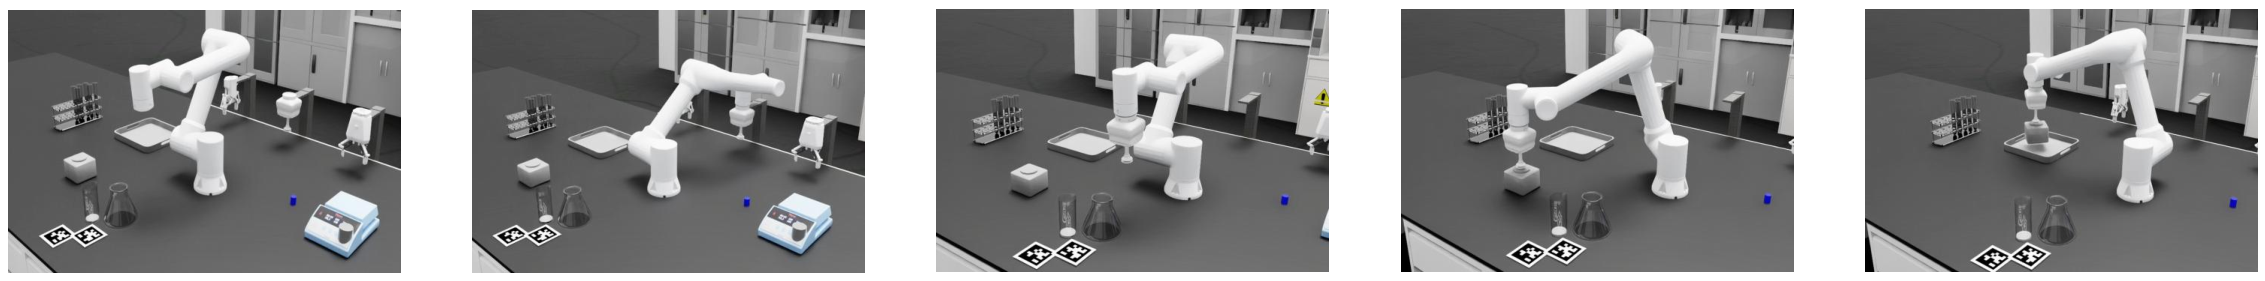
\includegraphics[width=0.95\textwidth]{figures/figure10a.pdf}}\\
\subfloat[\label{fig:fig.10b}]{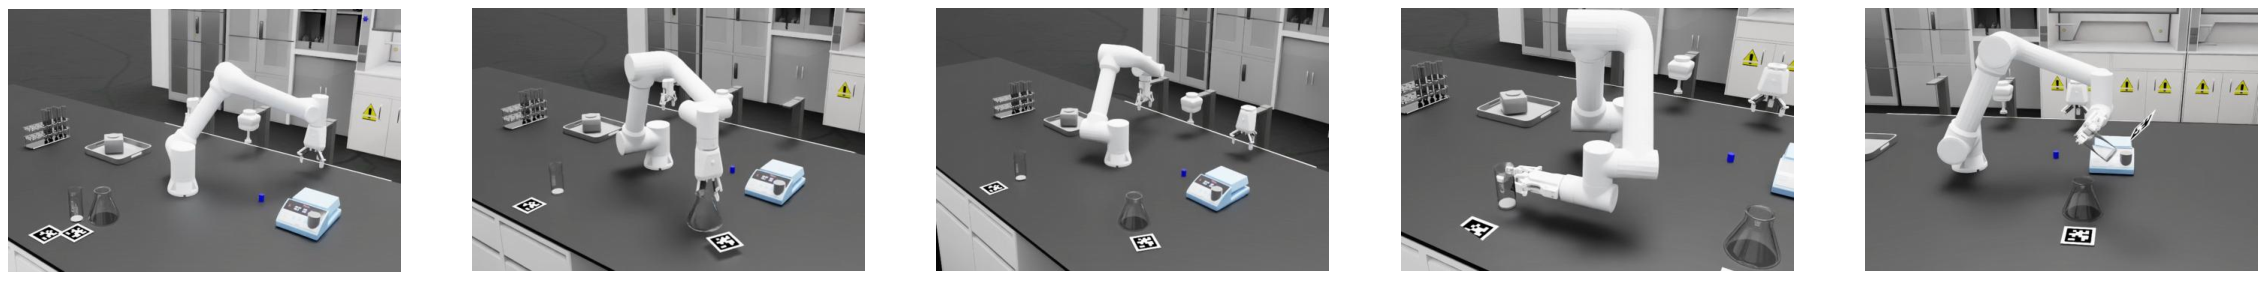
\includegraphics[width=0.95\textwidth]{figures/figure10b.pdf}}\\
\subfloat[\label{fig:fig.10c}]{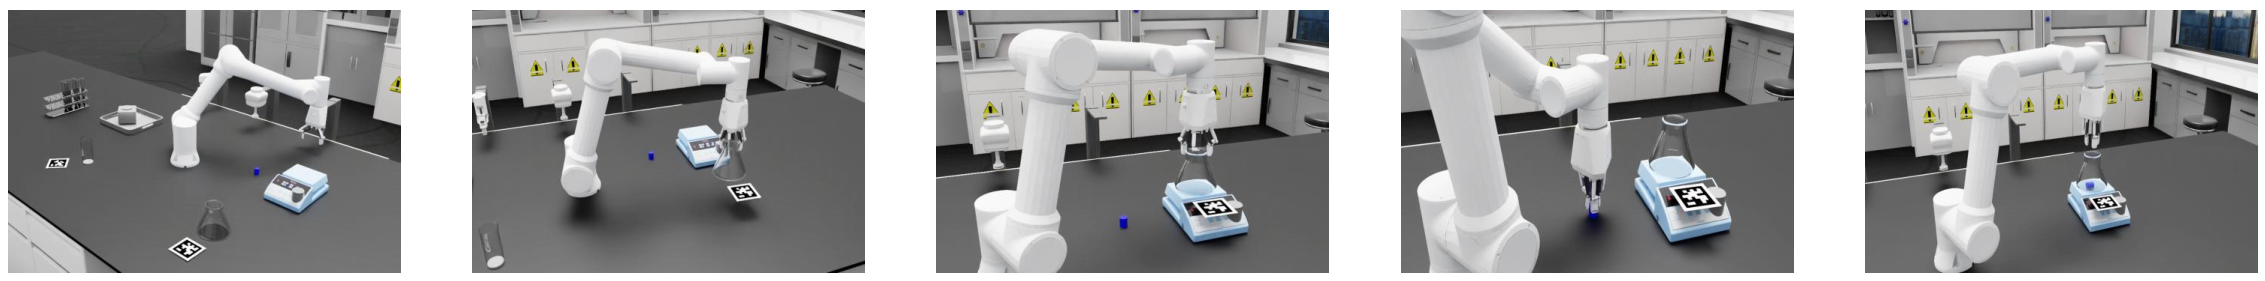
\includegraphics[width=0.95\textwidth]{figures/figure10c.pdf}}
\caption{Sequential execution snapshots of the Move $\rightarrow$ Transfer $\rightarrow$ Stir workflow evaluated in the end-to-end experiments. Each row shows five representative keyframes captured during a single trial. (a) Move: the robot relocates the container to the target zone. (b) Transfer: liquid reagent is poured into the destination vessel. (c) Stir: the mixture is stirred on the hotplate to complete the reaction sequence.}
\label{fig:fig.10}
\end{figure*}


\subsection{End-to-End System Evaluation}\label{sec:4.5}
While the preceding sections have verified planning reliability (Section \ref{sec:4.3}) and operational flexibility (Section \ref{sec:4.4}) independently, this section evaluates whether these capabilities are preserved when the modules operate as an integrated pipeline. A trial is counted as successful only when every procedural step completes in order, starting from a single natural language command\rev{, under the planning- and execution-success criteria of Section~\ref{sec:4.1.4}}; any failure at an intermediate step is treated as a complete trial failure. Each workflow is evaluated over 30 independent trials initialized with randomized World States and robot configurations.

To identify potential bottlenecks across the pipeline, end-to-end performance is decomposed into three sequential stages: XDL generation, in which the LLM Module translates the natural language command into a validated experimental protocol; planning, in which the TAMP Module produces a collision-free trajectory with LLM-guided tool selection and rearrangement; and execution, in which the Skill Library instantiates the planned trajectory into sensor-feedback-based motion primitives. As shown in Table \ref{tab:end_to_end}, XDL generation succeeds in 100\% of trials across all three workflows. Planning and execution each achieve 96.67\% on the two three-step workflows, with the Move $\rightarrow$ Transfer sequence reaching 100\% across all stages. \rev{The coincidence of planning and execution success rates indicates that the rigid-body execution of the planned trajectories introduced no additional failures under the phenomena the simulator models (Section~\ref{sec:4.1.4}); execution uncertainties outside the simulator, namely fluid dynamics and sensor latency, are characterized on the physical platform in Section~\ref{sec:4.6}.}




Representative execution snapshots of the Move $\rightarrow$ Transfer $\rightarrow$ Stir workflow are illustrated in Fig.~\ref{fig:fig.10}, showing the robot successfully completing all three procedural stages within a single trial. The overall average success rate of 97.78\% shows that the planning reliability and operational flexibility demonstrated in the preceding sections are preserved under integrated multi-step execution. End-to-end execution videos for all evaluated workflows are available on the project website at \url{https://rcilab.github.io/auto_chem}.

\subsection{Physical Validation on the FR5 Platform}\label{sec:4.6}
\rev{This section validates the physically deployable subset of the pipeline, comprising perception-derived state grounding, constrained planning, fixed-gripper execution, and adaptive pouring, on the physical FR5 manipulator described in Section~\ref{sec:4.1.1}.
The Transfer task is used throughout because it carries the tightest orientation constraints, is the task on which the planner comparison is most pronounced, and is the only task that requires closed-loop sensor-feedback execution; it is therefore the task on which the gap between simulation and hardware is largest.
Tool changing, which requires end-effectors not available on the physical platform, is not exercised on hardware (Section~\ref{sec:5.1}).}

\subsubsection{Perception Accuracy and Occlusion Robustness}\label{sec:4.6.1}
\rev{The dual-camera AprilTag pipeline of Section~\ref{sec:3.3.1} is evaluated against a 6-DoF reference at \nd{36} object poses, comprising three vessel types (beaker, flask, tube) in each of the 12 workspace grids.
The reference for each pose is obtained by probing three non-collinear points on the tag, its centre and two corners, with the robot tool tip; the probed points define the tag frame through forward kinematics and thus provide orientation as well as translation ground truth.
Table~\ref{tab:perception} reports the results.
Over the 36 poses the fused estimate has a mean translation error of \nd{2.1\,mm (maximum 4.6\,mm)} and a mean rotation error of \nd{1.2$^\circ$}, against \nd{2.9\,mm} and \nd{4.3\,mm} for the nearer and farther single camera respectively, confirming that inverse-distance fusion improves on either view alone.
Repeatability, measured separately as the standard deviation over 100 consecutive frames at each pose, is \nd{0.3\,mm}.
Occlusion robustness is evaluated under three conditions, camera~1 fully covered, camera~2 fully covered, and the tag \nd{50\%} covered in one view, each at \nd{12} poses with \nd{5} repetitions; detection continuity remained \nd{100\%} in all conditions and the fused error rose to \nd{3.1\,mm} under single-camera fallback.
The 36 measured 6-DoF residuals are the noise source for the perturbed-state planning evaluation of Section~\ref{sec:4.3}.}

\begin{table}[t]
\revbox{%
\centering
\caption{Localization accuracy of the perception pipeline on the physical platform against a probed 6-DoF reference (36 poses; occlusion conditions at 12 poses with 5 repetitions each).}\label{tab:perception}
\scriptsize
\setlength{\tabcolsep}{2pt}
\begin{tabular*}{\linewidth}{@{\extracolsep{\fill}}p{0.4\linewidth}cccc@{}}
\toprule
Condition & \makecell{Trans.\\mean (mm)} & \makecell{Trans.\\max (mm)} & \makecell{Rot.\\mean ($^\circ$)} & \makecell{Contin.\\(\%)} \\
\midrule
Camera 1 only & \nd{2.9} & \nd{6.1} & \nd{1.6} & \nd{100} \\
Camera 2 only & \nd{4.3} & \nd{8.7} & \nd{2.1} & \nd{100} \\
Fused (both views) & \nd{2.1} & \nd{4.6} & \nd{1.2} & \nd{100} \\
Fused, one camera covered & \nd{3.1} & \nd{6.4} & \nd{1.7} & \nd{100} \\
Fused, tag 50\% covered (one view) & \nd{2.6} & \nd{5.2} & \nd{1.4} & \nd{100} \\
Repeatability (1$\sigma$, 100 frames) & \nd{0.3} & -- & \nd{0.2} & -- \\
\bottomrule
\end{tabular*}}
\end{table}

\subsubsection{End-to-End Transfer from Natural Language}\label{sec:4.6.2}
\rev{\nd{Twenty} Transfer trials were executed end to end from a natural-language command, with the World State grounded by the physical cameras at every stage boundary, the Action Reasoner selecting the mounted 2-finger gripper in every trial so that no tool change was required, cuTAMP planning the SidePick--MoveHolding--Pour sequence, and the Adaptive Pouring skill closing the loop on the scale.
Source and target vessel placements were randomized across the grid in each trial.
Planning succeeded in \nd{20 of 20} trials and execution in \nd{19 of 20} (\nd{95.0\%}, Wilson 95\% CI \nd{76.4--99.1\%}) under the criteria of Section~\ref{sec:4.1.4}, with no collision and no spillage during transport in any trial; \nd{the single failure was a grasp slip during the tilt that left the poured mass outside the tolerance and was detected by the scale}.
\nd{In 8 of the 20 trials the Action Reasoner requested rearrangement of a blocking test tube, which was executed with the mounted gripper; all 8 rearrangements succeeded.}
Execution success on hardware is within \nd{one trial} of the simulated rate for the same task, which quantifies the gap introduced by the phenomena the simulator does not model.
Fig.~\ref{fig:hw} shows keyframes of a representative trial.}

\begin{figure*}[!t]
\centering
\revbox{%
\fbox{\parbox[c][0.26\linewidth][c]{\dimexpr\linewidth-2\fboxsep-2\fboxrule\relax}{\centering\nd{Figure placeholder: five keyframes of one physical Transfer trial on the FR5 (natural-language command, perception-grounded World State, SidePick, MoveHolding, adaptive pouring on the scale), to be captured during the hardware trials.}}}
\caption{Keyframes of a representative end-to-end Transfer trial on the physical FR5 platform: the World State is grounded by the two cameras, the 2-finger gripper side-grasps the source vessel, the MoveHolding trajectory keeps the vessel upright, and the Adaptive Pouring skill closes the loop on the electronic scale until the target mass is reached.}
\label{fig:hw}}
\end{figure*}

\subsubsection{Adaptive Pouring Accuracy}\label{sec:4.6.3}
\rev{The Adaptive Pouring skill was evaluated against the electronic scale for target volumes of 5, 10, and 20\,mL with 10 trials each, using water and a glycerol--water mixture (\nd{80\,wt\%, 22$^\circ$C, 1.21\,g/mL, 60\,mPa$\cdot$s}) as a viscous reagent, with the same PD gains for both liquids.
The end-to-end latency of the scale, measured by stepping a known mass, is \nd{95\,ms}, and the gains were tuned with this delay in the loop.
Table~\ref{tab:pouring} reports the results.
The mean absolute transfer error is \nd{0.42\,g} for water and \nd{0.71\,g} for the viscous liquid, overshoot stayed below \nd{1.0\,g} in every trial, and the mass settled within \nd{2.8\,s} of reaching the target; all 60 pours are within the \nd{1\,g} tolerance of the protocol.
These results provide quantitative evidence, under the tested conditions, for the sensor and fluid effects that the simulator does not model: scale settling and streaming latency, weight-signal noise, and viscosity-dependent flow.}

\begin{table}[t]
\revbox{%
\centering
\caption{Adaptive pouring accuracy on the physical platform (10 trials per liquid and target volume; same PD gains for both liquids).}\label{tab:pouring}
\scriptsize
\setlength{\tabcolsep}{2pt}
\begin{tabular*}{\linewidth}{@{\extracolsep{\fill}}llcccc@{}}
\toprule
Liquid & \makecell{Target\\(mL)} & \makecell{MAE\\(g)} & \makecell{Max err.\\(g)} & \makecell{Max over-\\shoot (g)} & \makecell{Settling\\(s)} \\
\midrule
\multirow{3}{*}{Water} & 5 & \nd{0.35} & \nd{0.7} & \nd{0.6} & \nd{2.4} \\
 & 10 & \nd{0.41} & \nd{0.8} & \nd{0.8} & \nd{2.7} \\
 & 20 & \nd{0.50} & \nd{0.9} & \nd{0.9} & \nd{3.1} \\
\midrule
\multirow{3}{*}{\makecell[l]{Glycerol--water\\(\nd{80\,wt\%})}} & 5 & \nd{0.62} & \nd{0.8} & \nd{0.7} & \nd{2.6} \\
 & 10 & \nd{0.70} & \nd{0.9} & \nd{0.8} & \nd{2.9} \\
 & 20 & \nd{0.81} & \nd{0.9} & \nd{0.9} & \nd{3.3} \\
\bottomrule
\end{tabular*}}
\end{table}

\subsubsection{Upright-Constraint Threshold}\label{sec:4.6.4}
\rev{The tilt limit $\theta_{\max}$ of the MoveHolding operator was grounded by a spillage sweep on the physical platform.
MoveHolding trajectories were executed with the beaker and the flask at fill levels of 30, 50, and 70\%, under tilt limits of 5, 10, and 15$^\circ$, five trials per condition, all with identical velocity and acceleration limits (\nd{0.25\,m/s and 0.5\,m/s$^2$}).
Spillage is declared when the mass loss between weighings before and after transport exceeds \nd{three times the repeatability of the scale (0.03\,g)}; the vessel exterior is wiped before each weighing, and evaporation over the trial interval is bounded by a stationary control vessel weighed over the same interval.
Table~\ref{tab:spill} reports the number of spilling trials per condition.
\nd{No spillage occurred at 5$^\circ$ at any fill level; at 10$^\circ$ spillage occurred only at 70\% fill, in 2 of 5 beaker trials and 1 of 5 flask trials; at 15$^\circ$ it occurred at every fill level of 50\% and above.}
The 5$^\circ$ threshold is therefore the largest tested tilt with zero spillage at the highest fill level used in the protocols; water is the conservative test liquid, since a more viscous liquid sloshes less at these tilt angles.}

\begin{table}[t]
\revbox{%
\centering
\caption{Spilling trials out of 5 (beaker / flask) by fill level and tilt limit during MoveHolding transport on the physical platform.}\label{tab:spill}
\begin{tabular*}{\linewidth}{@{\extracolsep{\fill}}lccc@{}}
\toprule
Fill level & $\theta_{\max}=5^\circ$ & $\theta_{\max}=10^\circ$ & $\theta_{\max}=15^\circ$ \\
\midrule
30\% & \nd{0 / 0} & \nd{0 / 0} & \nd{0 / 0} \\
50\% & \nd{0 / 0} & \nd{0 / 0} & \nd{4 / 3} \\
70\% & \nd{0 / 0} & \nd{2 / 1} & \nd{5 / 5} \\
\bottomrule
\end{tabular*}}
\end{table}

\section{Discussion and Limitations}\label{sec:5}
The experimental results in Section \ref{sec:4} validate the proposed framework within a high-fidelity simulation testbed \rev{and, for the physically deployable subset of the pipeline, on the physical manipulator}.
This section discusses the assumptions and limitations that bound the interpretation of those results, focusing on four aspects: sim-to-real transfer of the execution layer, perception robustness under realistic laboratory conditions, generalization of the LLM components beyond the training distribution, and system-level error propagation.

\subsection{Sim-to-Real Transfer and Physical Execution Uncertainty}\label{sec:5.1}
All quantitative results reported in \rev{Sections~\ref{sec:4.2}--\ref{sec:4.5}} were obtained in \textit{NVIDIA Isaac Sim}, which provides high-fidelity rigid-body kinematics and contact simulation but abstracts away the fluid-dynamic phenomena that dominate real-world liquid handling, including sloshing during transport, viscosity-dependent flow rates, and meniscus effects near vessel rims. The reported success rates for the Transfer task \rev{in simulation} should therefore be interpreted as evidence of geometric and kinematic feasibility, namely collision-free, orientation-constrained trajectory generation and valid pouring configurations\rev{; the quantitative liquid-transfer accuracy of the deployed skill is established on the physical platform in Section~\ref{sec:4.6.3}}.

The design of the Adaptive Pouring skill reflects this distinction. Precisely because analytical flow prediction is unreliable across reagents of varying viscosity, the skill does not depend on a fluid model: it closes the control loop on the measured weight from the electronic scale and adjusts the wrist angular velocity through a PD controller until the target mass is reached. This measurement-driven structure is consistent with sensor-feedback pouring systems that have been demonstrated on physical robots \cite{ref21, ref22}. \rev{The physical experiments of Section~\ref{sec:4.6} characterize how each fluid and sensor property enters this loop.
Viscosity changes the flow rate for a given tilt and therefore the effective plant gain; the mean absolute error rises from \nd{0.42\,g} for water to \nd{0.71\,g} for the \nd{60\,mPa$\cdot$s} glycerol mixture under the same PD gains, and overshoot stayed below \nd{1.0\,g} in both cases.
Sloshing matters during transport rather than pouring; the upright constraint and the acceleration limit on MoveHolding segments suppress it, and the spillage sweep of Section~\ref{sec:4.6.4} shows no spillage at $\theta_{\max}=5^\circ$ up to \nd{70\%} fill.
Surface tension delays the onset of flow at the rim and produces a residual drip after the tilt is reversed; the loop absorbs this as a dead time and a small late mass increment, which the measured overshoot bound includes.
Scale latency, measured at \nd{95\,ms} end to end, is compensated by tuning the gains with the delay in the loop and by a tilt-rate limit that keeps the mass poured during one latency interval below the tolerance.
Reagents far outside the tested viscosity range or vessels with markedly different rim profiles would require re-tuning the gains and the tilt-rate limit, which the modular structure of the framework confines to the skill layer without affecting the LLM and TAMP Modules.}

\rev{The hardware validation covers the physically deployable subset of the pipeline, namely perception-derived state grounding, constrained planning, fixed-gripper execution, and adaptive pouring.
Tool changing and device operation are validated in simulation only: the physical platform carries a single fixed 2-finger gripper, so the Automatic Tool Changing skill and the electromagnetic coupling sequence of Section~\ref{sec:3.5.1} were not exercised on hardware, and the claims for these two skills are limited to their simulated behaviour.
The tool-selection accuracy of the Action Reasoner (Table~\ref{tab:tool_selection}) is an inference result and is unaffected by this scope.}

\subsection{Perception Robustness under Realistic Laboratory Conditions}\label{sec:5.2}
The Perception Module assumes that fiducial markers remain detectable throughout operation. In a working chemistry laboratory this assumption can be violated: markers may degrade through chemical spills, condensation, or thermal exposure near hotplates, and may be transiently occluded by the manipulator or by relocated vessels. \rev{The design responds at three levels.
Under transient single-view obscuration, such as steam or the manipulator crossing one camera's view, the fusion rule falls back to the unobscured view (Section~\ref{sec:3.3.1}); in the occlusion test of Section~\ref{sec:4.6.1} this preserved \nd{100\%} detection continuity with a fused error of \nd{3.1\,mm}.
Under obscuration in both views during motion, no planning input is consumed, so the last validated pose is retained for monitoring only and is never used to plan.
At a stage boundary, every object involved in the next procedure must be freshly detected (Section~\ref{sec:3.3.2}); the system waits up to \nd{5\,s} and, if no valid detection is obtained in either view, halts and reports the affected object rather than planning on stale geometry.
This fail-closed rule covers persistent obscuration by condensation or chemical residue as well as transient obscuration that outlasts the wait.}

\rev{Operationally, tags are laminated and mounted on the vessel wall away from the rim and from heated surfaces, which keeps condensation and splashes off the tag in practice, and the fixed camera extrinsics are recalibrated periodically to bound calibration drift}; the inverse-distance weighting additionally suppresses the influence of the more distant, and typically less accurate, view. The fixed tag-to-object offset transform assumes rigid vessels with known marker placement, which holds for standard labware but requires re-registration whenever markers are re-affixed. Likewise, the simplified geometric primitives used for collision modeling trade fidelity for tractability; because non-target obstacles are enlarged conservatively, approximation errors bias the planner toward rejecting marginal plans rather than toward collision, at the cost of occasional infeasibility in tightly cluttered scenes.
Replacing fiducial tracking with marker-free 6-DoF pose estimation\rev{, for which learned estimators that adapt continually to new deployment domains are emerging \cite{peng2026lifelong}}, and cross-checking geometric state against instrument-level feedback in the spirit of closed-loop quality control \cite{khan2025real}, are natural extensions that would relax these operational constraints.

\subsection{Generalization of the LLM Components beyond the Training Distribution}\label{sec:5.3}
Both LLM components are fine-tuned on combinatorially constructed datasets, and the evaluations in Section \ref{sec:4} probe generalization only partially: test instructions include synonym and sentence-structure variations unseen during training, and tool selection is evaluated on object types absent from fine-tuning, but all evaluated commands remain within the six-operator XDL schema and the 12-grid workspace abstraction.
\rev{All generalization claims in this paper are accordingly restricted to that schema and workspace; extension to new operators or apparatus requires re-training on an extended dataset.}
Three out-of-distribution regimes therefore remain uncharacterized. Chemically ambiguous instructions, such as underspecified volumes or vessels, currently yield a generated protocol whose violated preconditions are intercepted by the XDL Validator, which halts execution and reports the offending step; this converts silent misinterpretation into an explicit rejection, but a systematic benchmark across ambiguity classes is left to future work. \rev{Adversarial or out-of-schema prompts are contained not by the decoder, which is not grammar-constrained, but by the deterministic validator, which rejects any operator outside the XDL vocabulary before planning; the adversarial test of Section~\ref{sec:4.2.2} intercepted \nd{all 60} invalid instructions, and the \nd{10} ambiguous-but-valid commands that passed validation delimit the residual exposure: an instruction that is schema-valid and precondition-consistent yet does not express the user's intent is executed as written.
Likewise, the XDL Validator covers syntactic, object-existence, and symbolic state-precondition failures\nd{, including vessel capacity and device placement}; chemical incompatibility, contamination constraints, and other conditions that require chemical knowledge are outside its scope, and unreachable configurations are resolved downstream by the TAMP Module, which reports infeasibility after the bounded retries.} Vessel geometries outside the training axes are partially covered by the unseen-object results in Table \ref{tab:tool_selection}, where semantic affordance grounding transferred to unseen vessel types; substantially novel apparatus such as separatory funnels or condensers would, however, require extending both the operator schema and the end-effector inventory. Finally, the choice of a 1B-parameter backbone was driven by inference latency rather than by a capability comparison across model scales; establishing the minimum model capacity required for reliable protocol generation and action reasoning remains an open question.

\subsection{Error Propagation and System-Level Robustness}\label{sec:5.4}
The hierarchical pipeline raises the concern that errors in early modules propagate downstream. The framework contains such propagation through three mechanisms, each exercised in Section \ref{sec:4}. First, the XDL Validator rejects invalid protocols before any physical planning begins, intercepting 100\% of injected errors \rev{of the tested classes} (Table \ref{tab:xdl_validator_cm}), so language-level failures terminate at the language layer \rev{(Section~\ref{sec:3.2.4} details the layered containment)}. Second, the stage-wise World State refresh before and after every procedure (Algorithm \ref{algo:tamp}) re-grounds planning in observed geometry, preventing pose errors from accumulating across stages. Third, bounded retry with re-initialization at both the task- and motion-planning levels absorbs transient planning failures, and unrecoverable failures halt the workflow with a diagnostic message rather than proceeding on an invalid plan. The end-to-end decomposition in Table \ref{tab:end_to_end} provides empirical evidence that these mechanisms are effective: planning and execution success rates coincide across all workflows, indicating that no additional failure modes \rev{emerged at the execution layer under the phenomena the simulator models}, and the observed incompletions correspond to isolated planning failures rather than cascaded module errors.

Two design choices deserve a precise reading in this context. The 12-grid workspace discretization reduces the output space of the Action Reasoner to a reliably learnable discrete set without limiting final placement precision, because exact coordinates are resolved by cuTAMP in continuous space; the category-level destination accuracy of 100\% (Table \ref{tab:action_reasoner}) supports this division of labor, and a finer grid would enlarge the symbolic output space and dilute per-cell training coverage without changing the continuous placement mechanism. Similarly, the bounded-latency property of the TAMP Module should be read as a per-attempt bound: the batched solver executes a fixed number of optimization steps over a fixed particle budget, so each planning attempt terminates within a bounded budget by construction, \rev{as reflected in the narrow band of termination times in Table~\ref{tab:tamp_comparison} and Fig.~\ref{fig:km}; the property concerns the predictability of termination rather than mean speed, since the baseline is faster on the configurations it does solve}; end-to-end wall-clock time additionally includes up to three re-planning attempts in the failure path.

\section{Conclusion}\label{sec:6}
This paper identified three coupled limitations that prevent existing approaches from achieving flexible and reliable chemistry laboratory automation: existing automation pipelines require manual redesign whenever new apparatus or procedures are introduced; constrained motion planning on low-redundancy manipulators suffers from degraded reliability and unpredictable termination time under orientation constraints; and LLM-based robot planning systems remain confined to protocol generation without determining the execution context required at each procedural stage. To address all three simultaneously, we proposed the LLM-Guided Tool-Aware TAMP framework, which unifies LLM-based context-aware decision-making with batched joint differentiable optimization-based planning within a single end-to-end pipeline.

The LLM Module jointly addresses the first and third limitations. By converting natural-language commands into validated XDL protocols, it eliminates the need for manual protocol redesign. By further inferring the appropriate end-effector and obstacle rearrangement strategy from the current World State and procedural context, it extends the role of the LLM beyond protocol generation to execution-context determination, achieving 100\% tool selection accuracy on standard task--object conditions and 96.67\% sequence completion through context-aware obstacle positioning, even for object types absent from the training distribution\rev{, within the evaluated six-operator, 12-grid workspace}. The TAMP Module addresses the second limitation by replacing sequential parameter-binding with batched joint differentiable optimization, improving the planning success rate from 66.7\% to 100.0\% on the Transfer task where orientation constraints are most restrictive, while \rev{returning every plan within a bounded band of termination times} appropriate for time-sensitive chemical workflows.
Together, these capabilities enable the integrated framework to achieve a 97.78\% end-to-end success rate on long-horizon chemical workflows initiated from a single natural language command \rev{in simulation, and the physically deployable subset of the pipeline reaches \nd{95.0\%} execution success on \nd{20} end-to-end liquid-transfer trials on the physical manipulator with a mean pouring error of \nd{0.42\,g}}.

\rev{Future work will extend the physical validation to tool changing and device operation with the full end-effector inventory, expand the supported XDL operators and skill library to cover more complex chemical procedures such as titration, filtration, and centrifugation, and benchmark the LLM components across model scales and out-of-distribution instruction regimes.}


\section*{Appendix A: Experimental Parameters}
\setcounter{table}{0}
\renewcommand{\thetable}{A\arabic{table}}
\begin{table*}[!t]
\centering
\revbox{%
\caption{Experimental parameters for the proposed method and the baseline. Values in red are read from the released configuration files.}\label{tab:params}
\footnotesize
\begin{tabular*}{\linewidth}{@{\extracolsep{\fill}}p{0.2\linewidth}p{0.37\linewidth}p{0.37\linewidth}@{}}
\toprule
Item & Proposed (cuTAMP) & Baseline (PDDLStream) \\
\midrule
Software & cuTAMP \nd{(commit 0000000)}, Isaac Sim \nd{4.2.0}, ROS~2 \nd{Humble} & \nd{Public reference implementation (commit 0000000)}, FastDownward, adaptive algorithm \\
Hardware & \nd{Intel Core i9-13900K, NVIDIA RTX 4090, 64\,GB RAM}; optimization on the GPU & Same workstation; streams on \nd{a single CPU thread} \\
Compute framing & \multicolumn{2}{p{\dimexpr0.74\linewidth+2\tabcolsep\relax}}{System-level wall-clock comparison in deployment configuration on one workstation; not compute-normalized} \\
Simulation & \multicolumn{2}{p{\dimexpr0.74\linewidth+2\tabcolsep\relax}}{Isaac Sim \nd{4.2.0}; PhysX step \nd{1/60\,s}, \nd{4} substeps} \\
Workspace & \multicolumn{2}{p{\dimexpr0.74\linewidth+2\tabcolsep\relax}}{\nd{0.9\,m $\times$ 0.6\,m} table; \nd{0.6\,m $\times$ 0.45\,m} grid region of \nd{4 $\times$ 3} cells, \nd{0.15\,m} each; remainder holds tool rack and devices} \\
Randomization & \multicolumn{2}{p{\dimexpr0.74\linewidth+2\tabcolsep\relax}}{Object position \nd{$\pm$5\,cm} of cell centre, yaw \nd{$\pm$180$^\circ$}, robot joints \nd{$\pm$10$^\circ$} of home; seeds 0--29 per task, shared by both planners} \\
Collision geometry & \multicolumn{2}{p{\dimexpr0.74\linewidth+2\tabcolsep\relax}}{Boxes and cylinders; obstacles enlarged by \nd{10\,mm}, targets by \nd{0\,mm}} \\
Robot and controller & \multicolumn{2}{p{\dimexpr0.74\linewidth+2\tabcolsep\relax}}{Simulation: joint-position control at \nd{60\,Hz}; physical FR5: vendor servo interface at \nd{125\,Hz}; limits \nd{180$^\circ$/s, 360$^\circ$/s$^2$}} \\
Orientation constraint & \multicolumn{2}{p{\dimexpr0.74\linewidth+2\tabcolsep\relax}}{$\theta_{\max}=5^\circ$ on MoveHolding and Place} \\
Time budget & \multicolumn{2}{p{\dimexpr0.74\linewidth+2\tabcolsep\relax}}{60\,s wall-clock per planning attempt} \\
Optimization / search & 1,024 particles; 1,000 steps; \nd{Adam, learning rate $10^{-2}$}; weights \nd{$w_{\mathrm{coll}}=10$, $w_{\mathrm{up}}=5$, $w_{\mathrm{goal}}=1$}; collision cost at \nd{32} points per segment & Grasp sampler \nd{25 candidates}; placement \nd{uniform over target grid}; IK \nd{numerical, 10 attempts}; motion \nd{RRT-Connect, 50 restarts}; \nd{unlimited stream re-instantiation} \\
Retry / termination & 3 re-initializations on failure; fixed step count & Timeout at 60\,s; early termination when \nd{the maximum stream-complexity level is reached} \\
Parameter selection & \nd{Defaults of the reference implementation} & \nd{Sampler counts tuned on seeds 100--109, disjoint from evaluation} \\
Planning success & \multicolumn{2}{p{\dimexpr0.74\linewidth+2\tabcolsep\relax}}{Trajectory returned within budget satisfying all constraints at every evaluated point} \\
Execution success (simulation) & \multicolumn{2}{p{\dimexpr0.74\linewidth+2\tabcolsep\relax}}{No contact with non-target objects; grasp slip below \nd{5\,mm}; upright at every control step; terminal condition met (Move: \nd{10\,mm}, \nd{5$^\circ$}; Transfer: pour pose above target; Stir: bar inside vessel)} \\
Physical platform & \multicolumn{2}{p{\dimexpr0.74\linewidth+2\tabcolsep\relax}}{FR5 with 2-finger gripper; cameras \nd{Intel RealSense D435, 1280$\times$720, 30\,Hz}; scale \nd{A\&D EK-610i, 0.01\,g, 10\,Hz}; liquids: water, glycerol--water \nd{80\,wt\%}} \\
\bottomrule
\end{tabular*}}
\end{table*}

\begin{thebibliography}{00}

\bibitem{bib3} M. Seifrid \emph{et al.}, ``Autonomous chemical experiments: Challenges and perspectives on establishing a self-driving lab,'' \emph{Accounts Chem. Res.}, vol. 55, no. 17, pp. 2454--2466, 2022.

\bibitem{bib4} M. Abolhasani and E. Kumacheva, ``The rise of self-driving labs in chemical and materials sciences,'' \emph{Nature Synth.}, vol. 2, no. 6, pp. 483--492, 2023.

\bibitem{garrett2021integrated} C. R. Garrett, R. Chitnis, R. Holladay, B. Kim, T. Silver, L. P. Kaelbling, and T. Lozano-P\'erez, ``Integrated task and motion planning,'' \emph{Annu. Rev. Control Robot. Auton. Syst.}, vol. 4, no. 1, pp. 265--293, 2021.

\bibitem{wang2021learning} Z. Wang, C. R. Garrett, L. P. Kaelbling, and T. Lozano-P\'erez, ``Learning compositional models of robot skills for task and motion planning,'' \emph{Int. J. Robot. Res.}, vol. 40, no. 6--7, pp. 866--894, 2021.

\bibitem{bib2} N. Yoshikawa \emph{et al.}, ``Chemistry lab automation via constrained task and motion planning,'' \emph{arXiv:2212.09672}, 2022.

\bibitem{bib5} C. R. Garrett, T. Lozano-P\'erez, and L. P. Kaelbling, ``PDDLStream: Integrating symbolic planners and blackbox samplers via optimistic adaptive planning,'' in \emph{Proc. Int. Conf. Automated Planning Scheduling}, vol. 30, 2020, pp. 440--448.

\bibitem{kingston2019exploring} Z. Kingston, M. Moll, and L. E. Kavraki, ``Exploring implicit spaces for constrained sampling-based planning,'' \emph{Int. J. Robot. Res.}, vol. 38, no. 10--11, pp. 1151--1178, 2019.

\bibitem{shen2025differentiable} W. Shen, C. Garrett, N. Kumar, A. Goyal, T. Hermans, T. Lozano-Perez, and F. Ramos, ``Differentiable GPU-parallelized task and motion planning,'' in \emph{Proc. Robot., Sci. Syst. (RSS)}, 2025.

\bibitem{ref3} B. Burger \emph{et al.}, ``A mobile robotic chemist,'' \emph{Nature}, vol. 583, no. 7815, pp. 237--241, 2020.

\bibitem{ref4} H. Fakhruldeen, G. Pizzuto, J. Glowacki, and A. I. Cooper, ``ARChemist: Autonomous robotic chemistry system architecture,'' in \emph{Proc. Int. Conf. Robot. Autom. (ICRA)}, 2022, pp. 6013--6019.

\bibitem{ref7} A. M. Lunt \emph{et al.}, ``Modular, multi-robot integration of laboratories: An autonomous workflow for solid-state chemistry,'' \emph{Chem. Sci.}, vol. 15, no. 7, pp. 2456--2463, 2024.

\bibitem{ref21} M. Kennedy, K. Schmeckpeper, D. Thakur, C. Jiang, V. Kumar, and K. Daniilidis, ``Autonomous precision pouring from unknown containers,'' \emph{IEEE Robot. Autom. Lett.}, vol. 4, no. 3, pp. 2317--2324, 2019.

\bibitem{ref22} Y. Huang, J. Wilches, and Y. Sun, ``Robot gaining accurate pouring skills through self-supervised learning and generalization,'' \emph{Robot. Auton. Syst.}, vol. 136, 2021, Art. no. 103692.

\bibitem{ref23} N. Yoshikawa, G. D. Akkoc, S. Pablo-Garc\'ia, Y. Cao, H. Hao, and A. Aspuru-Guzik, ``Does one need to polish electrodes in an eight pattern? Automation provides the answer,'' \emph{Digit. Discovery}, vol. 4, no. 2, pp. 326--330, 2025.

\bibitem{khan2025real} S. U. Khan, V. K. M\o ller, R. J. N. Frandsen, and M. Mansourvar, ``Real-time AI-driven quality control for laboratory automation: A novel computer vision solution for the Opentrons OT-2 liquid handling robot,'' \emph{Appl. Intell.}, vol. 55, no. 7, 2025, Art. no. 524.

\bibitem{ref13} R. I. C. Muchacho, R. Laha, L. F. C. Figueredo, and S. Haddadin, ``A solution to slosh-free robot trajectory optimization,'' in \emph{Proc. IEEE/RSJ Int. Conf. Intell. Robots Syst. (IROS)}, 2022, pp. 223--230.

\bibitem{ref11} Z. Kingston, M. Moll, and L. E. Kavraki, ``Sampling-based methods for motion planning with constraints,'' \emph{Annu. Rev. Control Robot. Auton. Syst.}, vol. 1, no. 1, pp. 159--185, 2018.

\bibitem{ref15} D. Coleman, I. Sucan, S. Chitta, and N. Correll, ``Reducing the barrier to entry of complex robotic software: A MoveIt! case study,'' \emph{arXiv:1404.3785}, 2014.

\bibitem{li2025dynamic} Y. Li, L. Ke, and C. Zhang, ``Dynamic obstacle avoidance and grasping planning for mobile robotic arm in complex environment based on improved TD3,'' \emph{Appl. Intell.}, vol. 55, no. 11, 2025, Art. no. 776.

\bibitem{kawaharazuka2025vision} K. Kawaharazuka, J. Oh, J. Yamada, I. Posner, and Y. Zhu, ``Vision-language-action models for robotics: A review towards real-world applications,'' \emph{IEEE Access}, vol. 13, pp. 162467--162504, 2025.

\bibitem{peng2025navigscene} \rev{Q. Peng \emph{et al.}, ``NavigScene: Bridging local perception and global navigation for beyond-visual-range autonomous driving,'' in \emph{Proc. 33rd ACM Int. Conf. Multimedia (MM)}, 2025.}

\bibitem{ref18} S. H. M. Mehr, M. Craven, A. I. Leonov, G. Keenan, and L. Cronin, ``A universal system for digitization and automatic execution of the chemical synthesis literature,'' \emph{Science}, vol. 370, no. 6512, pp. 101--108, 2020.

\bibitem{ref17} N. Yoshikawa \emph{et al.}, ``Large language models for chemistry robotics,'' \emph{Auton. Robots}, vol. 47, no. 8, pp. 1057--1086, 2023.

\bibitem{darvish2025organa} K. Darvish \emph{et al.}, ``ORGANA: A robotic assistant for automated chemistry experimentation and characterization,'' \emph{Matter}, vol. 8, no. 2, 2025.

\bibitem{ref19} A. M. Bran, S. Cox, O. Schilter, C. Baldassari, A. D. White, and P. Schwaller, ``ChemCrow: Augmenting large-language models with chemistry tools,'' \emph{arXiv:2304.05376}, 2023.

\bibitem{ref20} D. A. Boiko, R. MacKnight, B. Kline, and G. Gomes, ``Autonomous chemical research with large language models,'' \emph{Nature}, vol. 624, no. 7992, pp. 570--578, 2023.

\bibitem{vemprala2024chatgpt} S. H. Vemprala, R. Bonatti, A. Bucker, and A. Kapoor, ``ChatGPT for robotics: Design principles and model abilities,'' \emph{IEEE Access}, vol. 12, pp. 55682--55696, 2024.

\bibitem{qu2026trtp} Y. Qu, X. Hu, F. Chen, and Z. Wei, ``TRTP: A three-stage robust task planning framework for open worlds via visual-language models and digital twin simulation,'' \emph{Appl. Intell.}, vol. 56, no. 4, 2026, Art. no. 107.

\bibitem{wang2016apriltag} J. Wang and E. Olson, ``AprilTag 2: Efficient and robust fiducial detection,'' in \emph{Proc. IEEE/RSJ Int. Conf. Intell. Robots Syst. (IROS)}, 2016, pp. 4193--4198.

\bibitem{sarmadi2019simultaneous} H. Sarmadi, R. Mu\~noz-Salinas, M. A. Berb\'is, and R. Medina-Carnicer, ``Simultaneous multi-view camera pose estimation and object tracking with squared planar markers,'' \emph{IEEE Access}, vol. 7, pp. 22927--22940, 2019.

\bibitem{lynch2017modern} K. M. Lynch and F. C. Park, \emph{Modern Robotics}. Cambridge, U.K.: Cambridge Univ. Press, 2017.

\bibitem{peng2026lifelong} \rev{Q. Peng, H. Xue, P. Wang, and C. Chen, ``Lifelong domain adaptive 3D human pose estimation,'' in \emph{Proc. AAAI Conf. Artif. Intell.}, vol. 40, no. 10, 2026, pp. 8358--8366.}

\end{thebibliography}

\begin{IEEEbiography}[{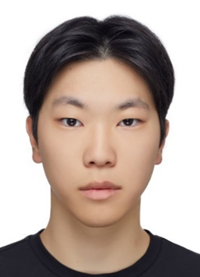
\includegraphics[width=1in,height=1.25in,clip,keepaspectratio]{figures/park.png}}]{Bohyeong Pak}
received the B.S. degree from the Department of Mechanical Engineering, Hanbat National University, in 2025. He is currently pursuing the M.S. degree with the Department of Mechanical Engineering, Kyung Hee University. His current research interests include collision avoidance, manipulation, and vision language model planning.
\end{IEEEbiography}

\begin{IEEEbiography}[{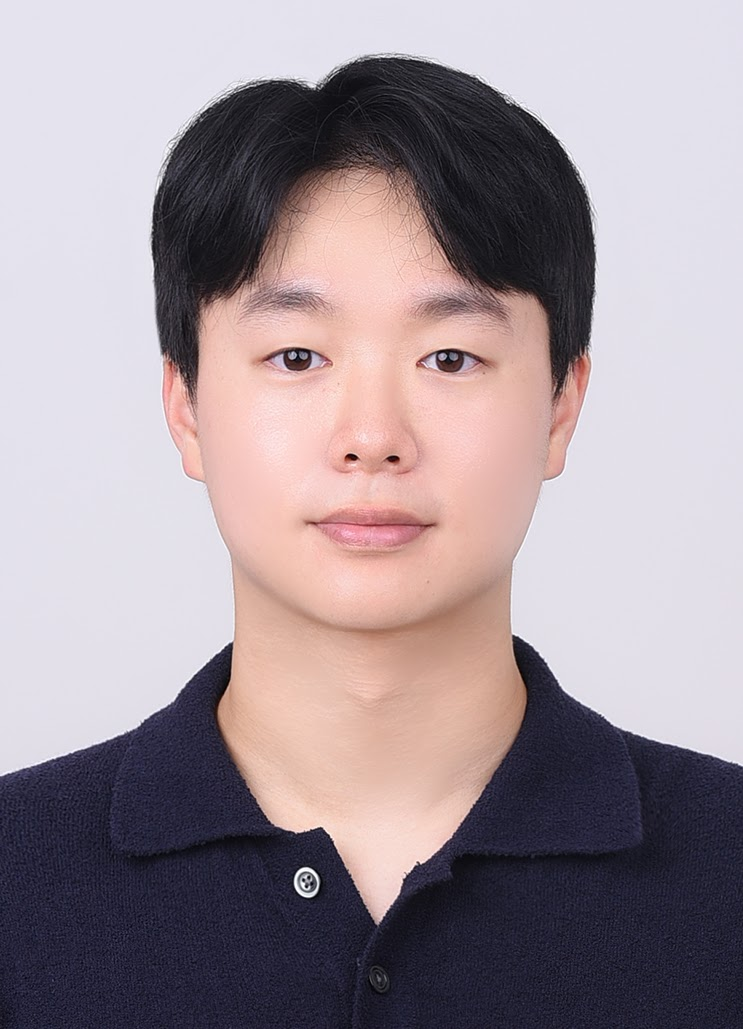
\includegraphics[width=1in,height=1.25in,clip,keepaspectratio]{figures/cho.jpg}}]{Hyunho Cho}
received the B.S. degree from the Department of Mechanical Engineering, Hanbat National University, in 2025. He is currently pursuing the M.S. degree with the Department of Mechanical Engineering, Kyung Hee University. His current research interests include optimal control and reinforcement learning.
\end{IEEEbiography}

\begin{IEEEbiography}[{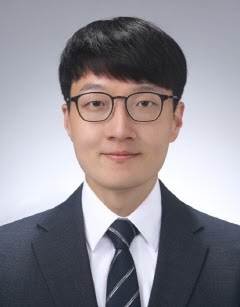
\includegraphics[width=1in,height=1.25in,clip,keepaspectratio]{figures/kim.jpg}}]{Sanghyun Kim}
(Member, IEEE) received the B.S. degree in mechanical engineering and the Ph.D. degree in intelligent systems from Seoul National University, South Korea, in 2012 and 2020, respectively. He was a Postdoctoral Researcher with The University of Edinburgh, U.K., in 2020, and a Senior Researcher with the Korea Institute of Machinery and Materials, South Korea, from 2020 to 2023. He is currently an Assistant Professor in mechanical engineering with Kyung Hee University. His main research interest includes the optimal control of mobile manipulators.
\end{IEEEbiography}

\EOD

\end{document}
